\documentclass[truedoublespace,tocchapterhead]{ccw_chithesis}
%\documentclass[tocchapterhead]{ccw_chithesis}
\usepackage{listings,amsmath,stmaryrd,pifont,../design/aux/bussproofs,esvect}
\usepackage{../design/aux/code,../design/aux/math-envs,../design/aux/math-cmds,../design/aux/code,../design/aux/proof}
\usepackage{pgf,pgfarrows,pgfnodes,tikz}
%\usepackage[pdftex]{graphicx}
\usepackage[top=1in, bottom=1.3in, left=1in, right=1in]{geometry}

%%%%%%%%%%%%%%%%%%%%%%%%%%%%%%%%%%%%%%%%%%%%%%%%%%%%%%%%%%%%%%%%%%%%%%
%% mac.tex
%%
%% Umut A. Acar
%% Macros for adaptive computation paper.
%%%%%%%%%%%%%%%%%%%%%%%%%%%%%%%%%%%%%%%%%%%%%%%%%%%%%%%%%%%%%%%%%%%%%%
\newcommand{\AFL}{\textsf{AFL}\xspace}
\newcommand{\IFL}{\textsf{IFL}\xspace}
\newcommand{\MFL}{\textsf{MFL}\xspace}
\newcommand{\AMFL}{\textsf{AMFL}\xspace}
%\newcommand{\SAL}{\textsf{SAL}\xspace}
\newcommand{\SLF}{\textsf{SLf}\xspace}
\newcommand{\SLI}{\textsf{SLi}\xspace}
\newcommand{\afl}{\AFL}
\newcommand{\ifl}{\IFL}
\newcommand{\mfl}{\MFL}
\newcommand{\amfl}{\AMFL}
%\newcommand{\sal}{\SAL}
\newcommand{\slf}{\SLF}
\newcommand{\sli}{\SLI}

\newcommand{\readarrow}{\ensuremath{\Longrightarrow}}


\newcommand{\cutspace}{\vspace{-4mm}}

\newcommand{\bomb}[1]{\fbox{\mbox{\emph{\bf {#1}}}}}

%\renewcommand{\paragraph}[1]{{\bf {#1}}}
% formatting stuff
\newcommand{\codecolsep}{1ex}

%\newcommand{\todo}[1]{{\bf{[NOTE:{#1}]}}}
\newcommand{\todo}[1]{}

\newcommand{\rlabel}[1]{\mbox{\small{\bf ({#1})}}}

\newcommand{\tablerow}{\\[5ex]}
\newcommand{\tableroww}{\\[7ex]}
\newcommand{\tableline}{
\vspace*{2ex}\\
\hline\\ 
\vspace*{2ex}}

% Don't care
\newcommand{\dontcare}{\_}


%% filter and quicksort stuff
\newcommand{\ncf}[2]{C^{fil}_{\ensuremath{{#1},{#2}}}}
\newcommand{\ncq}[1]{C^{qsort}_{\ensuremath{#1}}}
\newcommand{\nuf}[3]{P^{fil}_{#1,(\ensuremath{{#2},{#3}})}}
\newcommand{\nuq}[2]{P^{qsort}_{(\ensuremath{{#1},{#2}})}}

%% shorthands
\newcommand{\ddg}{{\sc ddg}}
\newcommand{\ncpa}{change-propagation algorithm}
\newcommand{\adg}{{\sc adg}}
\newcommand{\nwrite}{\texttt{write}}
\newcommand{\nread}{\texttt{read}}
\newcommand{\nmodr}{\texttt{mod}}
\newcommand{\ttt}[1]{\texttt{#1}}
\newcommand{\nmodl}{\texttt{modl}}
\newcommand{\nnil}{\ttt{NIL}}
\newcommand{\ncons}[2]{\ttt{CONS({\ensuremath{#1},\ensuremath{#2}})}}
\newcommand{\nfilter}{\texttt{filter}}
\newcommand{\nfilterp}{\texttt{filter'}}
\newcommand{\naqsort}{\texttt{qsort'}}
\newcommand{\nqsort}{\texttt{qsort}}
\newcommand{\nqsortp}{\texttt{qsort'}}
\newcommand{\nnewMod}{\texttt{newMod}}
\newcommand{\nchange}{\texttt{change}}
\newcommand{\npropagate}{\texttt{propagate}}
\newcommand{\ndest}{\texttt{d}}
\newcommand{\ninit}{\texttt{init}}



%% Comment sth out. 
\newcommand{\out}[1] {}
\newcommand{\sthat}{\ensuremath{~|~}}

%% definitions
\newcommand{\defi}[1]{{\bfseries\itshape #1}}


% Code listings.
\newcounter{codeLineCntr}
\newcommand{\codeLine}
 {\refstepcounter{codeLineCntr}{\thecodeLineCntr}}
\newcommand{\codeLineL}[1]
 {\refstepcounter{codeLineCntr}\label{#1}{\thecodeLineCntr}}

\newenvironment{codeListing}
 {\setcounter{codeLineCntr}{0}
%  \fontsize{10}{12}
 % the first one is width the second is height
 \fontsize{9}{11}
  \vspace{-.1in}
  \ttfamily\begin{tabbing}}
  {\end{tabbing}
   \vspace{-.1in}}

\newenvironment{codeListing8}
 {\setcounter{codeLineCntr}{0}
  \fontsize{8}{10}
  \vspace{-.1in}
  \ttfamily
  \begin{tabbing}}
 {\end{tabbing}
 \vspace{-.1in}
}

\newenvironment{codeListing8h}
 {\setcounter{codeLineCntr}{0}
  \fontsize{8.5}{10.5}
  \vspace{-.1in}
  \ttfamily
  \begin{tabbing}}
 {\end{tabbing}
 \vspace{-.1in}
}


\newenvironment{codeListing9}
 {\setcounter{codeLineCntr}{0}
  \fontsize{9}{11}
  \vspace{-.1in}
  \ttfamily
  \begin{tabbing}}
 {\end{tabbing}
 \vspace{-.1in}
}

\newenvironment{codeListing10}
 {\setcounter{codeLineCntr}{0}
  \fontsize{10}{12}
  \vspace{-.1in}
  \ttfamily
  \begin{tabbing}}
 {\end{tabbing}
 \vspace{-.1in}
}


\newenvironment{codeListingNormal}
 {\setcounter{codeLineCntr}{0}
  \vspace{-.1in}
  \ttfamily
  \begin{tabbing}}
 {\end{tabbing}
 \vspace{-.1in}
}

\newcommand{\codeFrame}[1]
{\begin{center}\fbox{\parbox[t]{5in}{#1}}\end{center}
% \vspace*{-.15in}
}

\newcommand{\fixedCodeFrame}[1]
{
\vspace*{-4mm}
\begin{center}
\fbox{
\vspace*{-2mm}
\parbox[t]{0.999\columnwidth}{
\vspace*{-2mm}
#1
}
}\end{center}
\vspace*{-4mm}
}

% Footnote commands.
\newcommand{\footnotenonumber}[1]{{\def\thempfn{}\footnotetext{#1}}}

% Margin notes - use \notesfalse to turn off notes.
\setlength{\marginparwidth}{0.6in}
\reversemarginpar
\newif\ifnotes
\notestrue
\newcommand{\longnote}[1]{
  \ifnotes
    {\medskip\noindent Note:\marginpar[\hfill$\Longrightarrow$]
      {$\Longleftarrow$}{#1}\medskip}
  \fi}
\newcommand{\note}[1]{
  \ifnotes
    {\marginpar{\raggedright{\tiny #1}}}
  \fi}

% Stuff not wanted.
\newcommand{\punt}[1]{}

% Sectioning commands.
\newcommand{\subsec}[1]{\subsection{\boldmath #1 \unboldmath}}
\newcommand{\subheading}[1]{\subsubsection*{#1}}
\newcommand{\subsubheading}[1]{\paragraph*{#1}}

% Reference shorthands.
\newcommand{\spref}[1]{Modified-Store Property~\ref{sp:#1}}
\newcommand{\prefs}[2]{Properties~\ref{p:#1} and~\ref{p:#2}}
\newcommand{\pref}[1]{Property~\ref{p:#1}}


\newcommand{\partref}[1]{Part~\ref{part:#1}}
\newcommand{\chref}[1]{Chapter~\ref{ch:#1}}
\newcommand{\chreftwo}[2]{Chapters \ref{ch:#1} and~\ref{ch:#2}}
\newcommand{\chrefthree}[3]{Chapters \ref{ch:#1}, and~\ref{ch:#2}, and~\ref{ch:#3}}
\newcommand{\secref}[1]{Section~\ref{sec:#1}}
\newcommand{\subsecref}[1]{Subsection~\ref{subsec:#1}}
\newcommand{\secreftwo}[2]{Sections \ref{sec:#1} and~\ref{sec:#2}}
\newcommand{\secrefthree}[3]{Sections \ref{sec:#1},~\ref{sec:#2},~and~\ref{sec:#3}}
\newcommand{\appref}[1]{Appendix~\ref{app:#1}}
\newcommand{\figref}[1]{Figure~\ref{fig:#1}}
\newcommand{\figreftwo}[2]{Figures \ref{fig:#1} and~\ref{fig:#2}}
\newcommand{\figpageref}[1]{page~\pageref{fig:#1}}
\newcommand{\tabref}[1]{Table~\ref{tab:#1}}
\newcommand{\stref}[1]{step~\ref{step:#1}}
\newcommand{\caseref}[1]{case~\ref{case:#1}}
\newcommand{\lineref}[1]{line~\ref{line:#1}}
\newcommand{\linereftwo}[2]{lines \ref{line:#1} and~\ref{line:#2}}
\newcommand{\linerefthree}[3]{lines \ref{line:#1},~\ref{line:#2},~and~\ref{line:#3}}
\newcommand{\linerefrange}[2]{lines \ref{line:#1} through~\ref{line:#2}}
\newcommand{\thmref}[1]{Theorem~\ref{thm:#1}}
\newcommand{\thmreftwo}[2]{Theorems \ref{thm:#1} and~\ref{thm:#2}}
\newcommand{\thmpageref}[1]{page~\pageref{thm:#1}}
\newcommand{\lemref}[1]{Lemma~\ref{lem:#1}}
\newcommand{\lemreftwo}[2]{Lemmas \ref{lem:#1} and~\ref{lem:#2}}
\newcommand{\lemrefthree}[3]{Lemmas \ref{lem:#1},~\ref{lem:#2},~and~\ref{lem:#3}}
\newcommand{\lempageref}[1]{page~\pageref{lem:#1}}
\newcommand{\corref}[1]{Corollary~\ref{cor:#1}}
\newcommand{\defref}[1]{Definition~\ref{def:#1}}
\newcommand{\defreftwo}[2]{Definitions \ref{def:#1} and~\ref{def:#2}}
\newcommand{\defpageref}[1]{page~\pageref{def:#1}}
%\newcommand{\eqref}[1]{Equation~(\ref{eq:#1})}
\newcommand{\eqreftwo}[2]{Equations (\ref{eq:#1}) and~(\ref{eq:#2})}
\newcommand{\eqpageref}[1]{page~\pageref{eq:#1}}
\newcommand{\ineqref}[1]{Inequality~(\ref{ineq:#1})}
\newcommand{\ineqreftwo}[2]{Inequalities (\ref{ineq:#1}) and~(\ref{ineq:#2})}
\newcommand{\ineqpageref}[1]{page~\pageref{ineq:#1}}
\newcommand{\itemref}[1]{Item~\ref{item:#1}}
\newcommand{\itemreftwo}[2]{Item~\ref{item:#1} and~\ref{item:#2}}

% Useful shorthands.
\newcommand{\abs}[1]{\left| #1\right|}
\newcommand{\card}[1]{\left| #1\right|}
\newcommand{\norm}[1]{\left\| #1\right\|}
\newcommand{\floor}[1]{\left\lfloor #1 \right\rfloor}
\newcommand{\ceil}[1]{\left\lceil #1 \right\rceil}
  \renewcommand{\choose}[2]{{{#1}\atopwithdelims(){#2}}}
\newcommand{\ang}[1]{\langle#1\rangle}
\newcommand{\paren}[1]{\left(#1\right)}
\newcommand{\prob}[1]{\Pr\left\{ #1 \right\}}
\newcommand{\expect}[1]{\mathrm{E}\left[ #1 \right]}
\newcommand{\expectsq}[1]{\mathrm{E}^2\left[ #1 \right]}
\newcommand{\variance}[1]{\mathrm{Var}\left[ #1 \right]}
\newcommand{\twodots}{\mathinner{\ldotp\ldotp}}

% Standard number sets.
\newcommand{\reals}{{\mathrm{I}\!\mathrm{R}}}
\newcommand{\integers}{\mathbf{Z}}
\newcommand{\naturals}{{\mathrm{I}\!\mathrm{N}}}
\newcommand{\rationals}{\mathbf{Q}}
\newcommand{\complex}{\mathbf{C}}

% Special styles.
\newcommand{\proc}[1]{\ifmmode\mbox{\textsc{#1}}\else\textsc{#1}\fi}
\newcommand{\procdecl}[1]{
  \proc{#1}\vrule width0pt height0pt depth 7pt \relax}
  \newcommand{\func}[1]{\ifmmode\mathrm{#1}\else\textrm{#1}fi} %
%  Multiple cases.  
\renewcommand{\cases}[1]{\left\{
  \begin{array}{ll}#1\end{array}\right.}
  \newcommand{\cif}[1]{\mbox{if $#1$}} 

%% spacing hacks
\newcommand{\longpage}{\enlargethispage{\baselineskip}}
\newcommand{\shortpage}{\enlargethispage{-\baselineskip}}

\newcommand{\ie}{\emph{i.e.}}
\newcommand{\etal}{\emph{et al.}}
\newcommand{\chk}{\ding{51}}
\newcommand{\ex}{\ding{55}}

\lstdefinelanguage{smlnj}{morekeywords={where},}

\lstloadlanguages{ML,[Objective]caml,smlnj}
\lstset{basicstyle=\footnotesize\sffamily,
        columns=fullflexible,
        %keywordstyle=\underbar,
		basewidth=0.55em,
		language=ML,
                alsolanguage=smlnj,
		numberstyle=\tiny,
	    mathescape=true,
		%aboveskip=0pt,
		%belowskip=-10pt
                lineskip=-8pt
		}
\newenvironment{lstlistingsingle}
{\begin{singlespace}\begin{lstlisting}}
{\end{lstlisting}\end{singlespace}}

		

%!TEX root = manual.tex
%
\chapter{ASDL Syntax}
\label{chap:syntax}

This section describes the syntax of the input language to \asdlgen{}.
The syntax is described using EBNF notation.
Literal terminals are typeset in \lit{bold} and enclosed in single quotes.
Optional terms are enclosed in square brackets and terms that are
repeated zero or more times are enclosed in braces.
Each section describes a fragment of the syntax and its meaning.

\section{Lexical Tokens}

The lexical conventions for \asdl{} are given in \figref{fig:lexical-syntax}.
ASDL is a case-sensitive language and, furthermore, classifies identifiers
into initial-lower-case (\synt{lc-id}) and initial-upper-case (\synt{uc-id}) identifiers.
Type identifiers are initial-lower-case, while constructor identifiers are initial-upper-case.
Module and field identifiers can be either upper or lower-case.

\begin{figure}[t]
  \begin{quote}
    \begin{grammar}
      <upper>     ::= `A' | ... | `Z'

      <lower>     ::= `a' | ... | `z'

      <alpha>     ::= `_' | <upper> | <lower>

      <alpha-num> ::= <alpha> | `0' | ... | `9'

      <lc-id>     ::= <lower> \{ <alpha-num> \}
      
      <uc-id>     ::= <upper> \{ <alpha-num> \}

      <id>        ::= <lc-id> | <uc-id>
                  
      <typ-id>    ::= <lc-id>

      <con-id>    ::= <uc-id>

      <comment>   ::= `--' \{ <text-character> \} <end-of-line>

      <text>      ::= `:' \{ <text-character> \} <end-of-line>
               \alt{} `\%\%' \{ <text-character> | <end-of-line> \} <end-of-line> `\%\%'
    \end{grammar}
  \end{quote}
  \caption{Lexical rules for \asdl{} terminals}
  \label{fig:lexical-syntax}
\end{figure}%

Comments begin with \lit{--}
and continue to the end of the line.

Verbatim text is denoted by \synt{text} and can be specified in one of two ways.
Either by an initial \lit{:} followed by a sequence of \synt{text-character}s that
continues to the end of the line or by a \lit{\%\%} terminated by a \lit{\%\%}
at the beginning of a line by itself. 
Text included using the `\lit{:} notation will have trailing and leading 
whitespace removed.

ASDL has the following keywords:
\begin{quote}
  \lit{alias}  \lit{attributes} \lit{import}
  \lit{include} \lit{module} \lit{primitive} \lit{view}
\end{quote}%
Note that it is allowed to use a keyword as an identifier wherever a \synt{lc-id} is permitted.

\section{File Syntax}

An \asdl{} file consists of one or more \synt{definition}s possibly preceded by \lit{include}
directives.
A definition specifies either a module (see \secref{sec:module-syntax}),
primitive module (see \secref{sec:primitive-syntax}),
or view (see \secref{sec:view-syntax}).

Include directives allow one to split a large \asdl{} specification into multiple files,
while allowing \asdlgen{} to check references from one module to another.
\asdlgen{} will parse included files, but will not generate code for the definitions in included
files.
Also, included files will only be parsed once.

\begin{figure}[t]
  \begin{quote}
    \begin{grammar}
      <file>  ::=  \{ `include' <text> \} <definition> \{ <definition> \}
      
      <definition> ::= <module>
        \alt{} <primitive-module>
        \alt{} <view>
    \end{grammar}
  \end{quote}
  \caption{\asdl{} file syntax}
  \label{fig:file-syntax}
\end{figure}%

\section{Module Syntax}
\label{sec:module-syntax}

\figref{fig:module-syntax} gives the syntax for modules.
An \asdl{} module declaration consists of the keyword \lit{module}
followed by an identifier, an optional set of imported modules, and a
sequence of type definitions enclosed in braces.

\begin{figure}[t]
  \begin{quote}
    \begin{grammar}
      <module>  ::=  `module' <id> [ <imports> ] `{' \{ <type-definition> \} `}'

      <imports> ::=  `(' \{ `import' <id> [ `alias' <id> ] \} `)'
    \end{grammar}
  \end{quote}
  \caption{\asdl{} module syntax}
  \label{fig:module-syntax}
\end{figure}%

For example the
following example declares modules \lstinline[language=ASDL]!A!,
\lstinline[language=ASDL]!B!, and \lstinline[language=ASDL]!C!.
\lstinline[language=ASDL]!B! imports types from \lstinline[language=ASDL]!A!.
\lstinline[language=ASDL]!C! imports types from both \lstinline[language=ASDL]!A! and
\lstinline[language=ASDL]!B!.
Imports cannot be recursive; for example, it is an error for \lstinline[language=ASDL]!B! to
import \lstinline[language=ASDL]!C!, since \lstinline[language=ASDL]!C!
imports \lstinline[language=ASDL]!B!.
\begin{code}\begin{lstlisting}[language=ASDL]
 module A { ... } 
 module B (import A) { ... }
 module C (import A 
           import B) { ... }
\end{lstlisting}\end{code}% 

To refer to a type imported from another module the type must
\emph{always} be qualified by the module name from which it is
imported.
The following declares two different types called ``\texttt{t}.''
One in module \texttt{A} and one in module \texttt{B}.
The type ``\texttt{t}'' in module \texttt{B} defines a type ``\texttt{t}'' that
recursively mentions itself and also references the type ``\texttt{t}'' imported
from module \texttt{A}.
\begin{code}\begin{lstlisting}[language=ASDL]
module A { t = ... } 
module B (import A) { t = T(A.t, t) | N  ... }
\end{lstlisting}\end{code}% 

\section{Type Definitions}

The syntax of type definitions is given in \figref{fig:type-syntax}.
A type defintion begins with a type identifier, which is the name of the type.
The name must be unique within the module, but the order of definitions is unimportant.
When translating type definitions from a module they are placed in what would be considered a
module, package, or name-space of the same name.
If the output language does not support such features and only has one global
name space the module name
is used to prefix all the globally exported identifiers.

\begin{figure}[t]
  \begin{quote}
    \begin{grammar}
      <type-definition>  ::=  <typ-id> `=' <type>

      <type>         ::= <alias-type> | <sum-type> | <product-type>

      <alias-type>   ::= <typ-exp>
      
      <product-type> ::= <fields>

      <sum-type>     ::= <constructor> \{ `|' <constructor> \} [ `attributes' <fields> ]

      <constructor>  ::= <con-id> [ <fields> ]

      <fields>       ::= `(' \{ <field>  `,' \} <field> `)'

      <field>        ::=  <typ-exp> [ <id> ]
      
      <typ-exp>      ::= [ <id> `.' ] <typ-id> [ `?' | `*' | `!' ]
    \end{grammar}
  \end{quote}
  \caption{\asdl{} type definition syntax}
  \label{fig:type-syntax}
\end{figure}%

Type definitions are either alias types, which bind a name to a type expression;
product types, which are simple record definitions;
or sum type, which represent a discriminated union of possible values.
Unlike sum types, product types cannot form recursive type definitions, but they can
contain recursively declared sum types.

\subsection{Alias Types}

Alias types are the simplest form of type definition.
They provide a way to give a name to a type or type expression, similar
to \sml{}'s \lstinline[language=SML]@type@ and \Cplusplus{}'s
\lstinline[language=C++]@typedef@ constructs.

\subsection{Type expressions}

A type expression (\synt{typ-exp}) consists of a possibly qualified type name followed
by an optional type operator.
If the specified type is an ASDL primitive type or is defined in the current module,
then its name is not qualified; all other types defined outside the current module must
be qualified by their module name (or module alias).

The type operators are:
\begin{itemize}
  \item
    option (\lit{?}), which specifies either zero or one value of the specified type.
  \item
    sequence (\lit{*}), which specifies a sequence of zero or more values of the
    specified type, or
  \item
    shared (\lit{!}), which specifies that a value is shared across multiple points
    in the data structure (\ie{}, the structure has a DAG shape instead of just a tree).
\end{itemize}%

Note that while at most one type operator is allowed in a type expression, one can use alias
types to combine two or more operators.
For example, a sequence of optional integers could be defined by:
\begin{code}\begin{lstlisting}[language=ASDL]
int_opt = integer?
int_opt_seq = int_opt*
\end{lstlisting}\end{code}%

\subsection{ASDL Primitive Types}
There are seven pre-defined primitive types in ASDL, which are available without qualification:
\begin{description}
  \item[\normalfont\texttt{\color{\cdColor}bool}] describes Boolean values.
  \item[\normalfont\texttt{\color{\cdColor}int}] describes signed-integer values that are representable in 30 bits
    (\ie{}, in the range ${-}2^{29}$ to~\mbox{$2^{29}-1$}).
  \item[\normalfont\texttt{\color{\cdColor}uint}] describes unsigned-integer values that representable in 30 bits
    (\ie{}, in the range $0$ to~$2^{30}-1$).
  \item[\normalfont\texttt{\color{\cdColor}integer}] describes arbitrary-precision signed-integer values.
  \item[\normalfont\texttt{\color{\cdColor}natural}] describes arbitrary-precision unsigned-integer values.
  \item[\normalfont\texttt{\color{\cdColor}string}] describes length encoded strings of 8-bit characters.
  \item[\normalfont\texttt{\color{\cdColor}identifier}] describes strings with fast equality testing
    analogous to Lisp symbols.
\end{description}%

% TODO: Not implemented yet
%In addition, the \lstinline!StdTypes! module defines additional fixed-precision numeric types
%that can be used when necessary (\eg{}, \lstinline!StdTypes.int32!).

\subsection{Product Types}
Product types are defined by a non-empty  sequence of fields separated by
commas enclosed in parenthesis.
A field consists of a type expression followed by an optional label.
The fields of a product or sum type must either all be labeled or unlabeled.
We use \emph{record} to refer to products of labeled fields and \emph{tuple}
to products of unlabeled fields.
Labels aid in the readability of
descriptions and are used by \asdlgen{} to name the fields of records
and classes for languages.

For example, the declaration
\begin{code}\begin{lstlisting}[language=ASDL] 
pair_of_ints = (int, int) 
\end{lstlisting}\end{code}% 
defines the tuple type \lstinline[language=ASDL]!pair_of_ints! that consists of two integers,
whereas the declaration
\begin{code}\begin{lstlisting}[language=ASDL] 
size = (int width, int height) 
\end{lstlisting}\end{code}%
defines the record type \lstinline[language=ASDL]!size! that consists of two
labeled fields: \lstinline[language=ASDL]@width@ and \lstinline[language=ASDL]@height@.
Note that ASDL requires that if any field in a product type has a label, then all
of them must have labels.

For the \sml{} target, product types without labels are translated to tuples, while
those with labels are translated to records.

\subsection{Sum Types}

Sum types are the most useful types in ASDL. They provide concise notation
used to describe a type that is the tagged union of a finite set of other
types.  Sum types consists of a series of constructors separated by a
vertical bar. Each constructor consist of a constructor identifier followed
by an optional product type. 

Constructor names must be unique within the module in which they are
declared. Constructors can be viewed as functions who take some number of
arguments of arbitrary type and create a value belonging to the sum type in
which they are declared.
For example
\begin{code}\begin{lstlisting}[language=ASDL]
module M {
  sexpr = Int(int)
	| String(string)
	| Symbol(identifier)
	| Cons(sexpr, sexpr)
	| Nil
}
\end{lstlisting}\end{code}%
declares that values of type \lstinline[language=ASDL]!sexpr! can either be
constructed from an \lstinline[language=ASDL]!int! using the
\lstinline[language=ASDL]!Int! constructor or a \lstinline[language=ASDL]!string!
from a \lstinline[language=ASDL]!String! constructor, an
\lstinline[language=ASDL]!identifier! using the \lstinline[language=ASDL]!Symbol!
constructor, from two other \lstinline[language=ASDL]!sexpr! using the
\lstinline[language=ASDL]!Cons! constructor, or from no arguments
using the \lstinline[language=ASDL]!Nil! constructor.
Notice that the \lstinline[language=ASDL]!Cons! constructor
recursively refers to the \lstinline[language=ASDL]!sexpr! type.
\asdl{} allows sum types to be mutually recursive.
Recursion, however, is limited to sum types defined within the same module.

\subsubsection{Sum Types as Enumerations}
\label{sec:enumerations}

Sum types that consist completely of nullary constructors
are often treated specially and translated into static constants of a
enumerated value in languages that support them.
For example, the following \asdl{} specification:
%
\begin{code}\begin{lstlisting}[language=ASDL]
module Op {
  op = PLUS | MINUS | TIMES | DIVIDE 
}
\end{lstlisting}\end{code}%
%
Is translated into the following \Cplusplus{} code:
%
\begin{code}\begin{lstlisting}[language=c++]
namespace M {
    enum class op {
        PLUS = 1, MINUS, TIMES, DIVIDE
    };
}
\end{lstlisting}\end{code}%

\subsubsection{Attribute Fields}
A sum-type definition may optionally be followed by a list of attribute fields, which
provide a concise way to specify fields that are common to all of the constructors
of a sum type.
For example, the definition
%
\begin{code}\begin{lstlisting}[language=ASDL]
module M {
  pos = (string file, int linenum, int charpos)
  sexpr = Int(int)
	| String(string)
	| Symbol(identifier)
	| Cons(sexpr, sexpr)
	| Nil
        attribute(pos)
}
\end{lstlisting}\end{code}%
adds a field of type \lstinline[language=ASDL]!pos! to all the constructors
in \lstinline[language=ASDL]!sexpr!.
One can think of an \lstinline!attribute! annotation as syntactic sugar for just including
the extra fields at the \emph{beginning} of each constructor's fields.
For example, the above definition can be viewed as syntactic sugar for
%
\begin{code}\begin{lstlisting}[language=ASDL]
module M {
  pos = (string file, int linenum, int charpos)
  sexpr = Int(pos, int)
	| String(pos, string)
	| Symbol(pos, identifier)
	| Cons(pos, sexpr, sexpr)
	| Nil(pos)
}
\end{lstlisting}\end{code}%
Note that this interpretation implies that attribute fields are labeled if, and only if, all
of the constructor fields are labeled.

Attribute fields are treated specially when translating to some targets.
For example in \Cplusplus{} code, the attribute field is defined in the base class for the sum type.

\section{Primitive Modules}
\label{sec:primitive-syntax}

\begin{figure}[t]
  \begin{quote}
    \begin{grammar}
      <primitive-module> ::= `primitive' `module' <id> `{' \{ <id> \} `}'
    \end{grammar}%
  \end{quote}%
  \caption{\asdl{} primitive module syntax}
  \label{fig:prim-module-syntax}
\end{figure}%

Primitive modules (see \figref{fig:prim-module-syntax}) provide a way to introduce abstract
types that are defined outside
of \asdl{} and which have their own pickling and unpickling code.
For example, we might want to include GUIDs (16-byte globally-unique IDs) in our pickles.
We can do so by first defining a primitive module \lstinline!Prim!:
%
\begin{quote}\begin{lstlisting}[language=ASDL]
primitive module Prim { guid }
\end{lstlisting}\end{quote}%
%
Then, depending on the target language, we define
supporting code to read and write guids from the byte stream.
In \sml{}, we would define two modules:
\begin{enumerate}
  \item \lstinline[language=SML]!structure Prim! that defines the representation of the
    \lstinline[language=SML]!guid! type.
  \item
    \lstinline[language=SML]!structure PrimPickle! that defines functions
    for pickling/unpickling a GUID using an imperative stream API.
\end{enumerate}%
The \sml{} implementation of these modules could be written as follows:
\begin{code}\begin{lstlisting}[language=SML]
structure Prim : sig
    type guid
  end = struct
    type guid = GUID.guid
  end

structure PrimPickle : sig

    val read_guid : (unit -> Word8.word) -> unit -> Prim.guid
    val write_guid : (Word8.word -> unit) -> Prim.guid -> unit
    
  end = struct
  
    val guidSize = 16
    fun read_guid getByte () =
          GUID.fromBytes(Word8Vector.tabulate(guidSize, fn _ => getByte()))
    fun write_guid putByte guid = let
          Word8Vector.app putByte (GUID.toBytes guid)

   end
\end{lstlisting}\end{code}%
(assuming that the \lstinline!GUID! module implements the application's representation
of GUIDs).

For \Cplusplus{}, a primitive module requires a corresponding header file that declares
the primitive types and instances of the overloaded \lstinline[language=c++]!<<! and
\lstinline[language=c++]!>>! operators on the primitive types.  These declarations should
all be in a \lstinline[language=c++]!namespace! with the type name of the primitive module.
For example, the module from above would require the provision of a \texttt{Prim.hxx} header
file that contained something like the following code:
%
\begin{code}\begin{lstlisting}[language=c++]
#include <iostream>
#include "guid.hxx"

namespace Prim {

    typedef GUID::guid guid;

    std::istream &operator>> (std::istream &is, guid &g);
    std::ostream &operator<< (std::ostream &os, guid const &g);

}
\end{lstlisting}\end{code}%
(assuming that the \texttt{guid.hxx} header defines the application's representation
of GUIDs).
%For the \Cplusplus{} target, one should use string streams (in binary mode)
%to support pickling/unpickling of to/from memory.


\section{View Syntax}
\label{sec:view-syntax}

A view defines how an \asdl{} specification is translated to a target.
Each of the supported targets (\eg{}, \sml{} or \Cplusplus{}) has a default
view, but it is possible to customize the translation using \synt{view}
definitions.
The syntax of view declarations is given in \figref{fig:view-syntax}.
This section covers the syntax of views, but leaves the semantics to
\chapref{chap:views}.

\begin{figure}[t]
  \begin{quote}
    \begin{grammar}
      <view>        ::= `view' <id> `{' \{ <view-entry> \} `}'

      <view-entry>  ::=  <view-entities> `<=' <view-properties>
         \alt{} `<=' <id> `{' \{ <view-entity> <text> \} `}'

      <view-entities> ::= <view-entity>
         \alt{} `{' \{ <view-entity> \} `}'

      <view-entity> ::= `<file>'
         \alt{} `module' <id>
         \alt{} <id> `.' <typ-id> [ `.' `*' ]
         \alt{} <id> `.' <typ-id> `.' <con-id>

      <view-properties> ::= <id> <text>
          \alt{} `{' \{ <id> <text> \} `}'
    \end{grammar}%
  \end{quote}%
  \caption{\asdl{} view syntax}
  \label{fig:view-syntax}
\end{figure}%

\subsection{Basic View Syntax}
Views are named and consist of series of entries.
In its basic form, a view entry consists of a \synt{view-entity}, which specifies a file, module,
type, or constructor entity, and a view property, which is a name-value pair that is associated with
the entity.
%
\begin{quote}\begin{grammar}
  <view-entry>  ::= <view-entity> `<=' <id> <text>
\end{grammar}\end{quote}%
%
The meaning of an entry is to associate the specified view property with the specified view entity.
%%
%\begin{code}\begin{lstlisting}[language=ASDL]
%view Doc {
%  module  M <= doc_string
%%%
%  Types for representing LISP s-expressions.
%%%
%  M.sexpr  <= doc_string : s-expressions 
%  M.Int    <= doc_string : s-expression constructor
%  M.Symbol <= doc_string : s-expression constructor
%  M.Cons   <= doc_string : s-expression constructor
%  M.Nil    <= doc_string : s-expression constructor
%}
%
%view Java {
% M.sexpr <= source_name : Sexpr
% M.sexpr <= base_class  : MyClass
%}
%\end{lstlisting}\end{code}%
%%
%associates with the module \lstinline[language=ASDL]!M! the type
%\lstinline[language=ASDL]!M.sexpr! and the
%constructor \lstinline[language=ASDL]!M.Int!
%strings that will be added to the automatically generated documentation
%produced by the \texttt{--doc} command of \asdlgen{}.
%(\emph{In future we will probably dump them in comments in the output code too.})
%The view named \lstinline[language=ASDL]!Java! causes the type
%\lstinline[language=ASDL]!M.sexpr! to be renamed \lstinline[language=ASDL]!Sexpr! when
%generating Java output, and causes the abstract class normally generated to
%inherit from \lstinline[language=ASDL]!MyClass!. 

There can be multiple views with the same name.
The entries of two views with the same name are merged and consist of the
union of the entries in both.
It is an error, for two views of the same name to assign different values
to the same property of an entity.

\subsection{View Entry Derived Forms}
To make it easier to specify view entries, \asdl{} generalizes the basic syntax
to remove some of the redundancy of the basic syntax.
First, it is possible to specify multiple view entities on the left-hand-side of
the \lit{<=} symbol.
Likewise, it is possible to specify multiple view properties on the right-hand-side
of the \lit{<=} symbol.

It is also possible to assign different values to different entities for a fixed property
using the syntax.
%
\begin{quote}\begin{grammar}
  <view-entry> ::= `<=' <id> `{' \{ <view-entity> <text> \} `}'
\end{grammar}\end{quote}%
%
Here the property name is given first, followed by a sequence of view-entity-value pairs.

Lastly, \asdl{} allows a \lit{.*} suffix to be added to sum-type entities.
This suffix means that the entity specifies the set of all of the constructors of the type.

%Examples of the sugared notation are shown
%below in their respective order.
%\begin{code}\begin{lstlisting}[language=ASDL]
%view Doc {
% { M.Int  M.Symbol  
%   M.Cons M.Nil } <= doc_string : s-expression constructor
%
% <= doc_string {
%  module  M 
%%%
%  Types for representing LISP s-expressions.
%%%
%  M.sexpr : s-expressions 
%  }
%}
%
%view Cxx {
%  M.sexpr <= {
%    source_name : Sexpr
%    base_class  : MyClass
%  }
%}
%\end{lstlisting}\end{code}%


\setcounter{tocdepth}{1}

\bibliographystyle{plain}

\begin{document}
	\title{A True Higher-Order Module System}
	\author{George Kuan}
	\department{Computer Science}
	\division{Physical Sciences}
	\degree{Doctor of Philosophy}
	\date{JUNE 2010}
	\maketitle
	\makecopyright
	  
	\dedication
	\begin{center}
		\emph{To my dearest wife}
                
	\end{center}
		  	    
	\tableofcontents
	\listoffigures
	%\listoftables

	\acknowledgments{Acknowledgments.}
                I owe a great debt of gratitude to my advisor, Dave
                MacQueen, who has guided me and taught me much of what
                I know about programming language semantics and module
                system semantics. His detailed feedback was very
                insightful and critical to the writing of this
                dissertation. I am also very thankful to John Reppy
                and Matthias Blume for serving on my committee and
                their helpful feedback. My special thanks goes out to my early 
                collaborator Robby Findler who pointed me to many opportunities 
                and taught me the ``street smarts'' of the academic world. 

                I cannot thank enough the rest of the Department of Computer Science and the Division of Physical Sciences for their tireless and superhuman effort in supporting me in my study. In particular, I would like to especially thank Nita Yack and Anne Rogers of the Department of Computer Science for working miracles. I thank Rick Hefley and Jennifer Woods from the Dean's Office of the Physical Science Division. My special thanks also goes out to Brooke Noonan of the Graduate Affairs Office. My thanks goes out to Sharon Salveter for her mentoring and guidance for the teaching aspect of my graduate career. I thank Margaret Jaffey for helping me out with the ins and outs of the formal requirements of graduate work. I also thank Donna Brooms for helping me in the numerous practical matters at the University. 

                My thanks goes out to my officemates Chunyan Song, Mike Rainey, Matthew 
                Jacobs, Adam Shaw, Aaron Turon, Ioan Raicu, and Jon Riehl. Thank you 
                for your good humor and insightful conversations. I
                also thank the other PLs students Lars Bergstrom and
                Casey Klein. The TTI-Chicago people were also
                extremely supportive and in many ways, their
                interesting ideas, vibrant energy, and feedback helped
                shape my research and enriched my graduate
                career. Special thanks are due to Umut Acar, Amal
                Ahmed, Wonseok Chae, Derek Dreyer, and Xinyu Feng. 

                I also have to thank the Mobile Software Labs researchers at DOCOMO Labs USA for inviting me to work on a research internship as part of their FAST Project for Automated Mobile Software specification, verification, and testing. I thank Ajay Chander, Dinakar Dhjurati, and Dachuan Yu. 

                As for my friends from church, the Lin family, Paul and Laura Chang, Li Chen, Ningzhong and
                Ying, Jason and Sue Montgomery, Isaac and Ariel Chen, Howard and Barb Perino, and Frankie Wong, thank you all for inviting me to your home week after week. Your faithfulness encouraged me in most difficult times. 
%I thank Grace Liu, Jinju Culp, Andy Lamb, and Leslie Mondrian for . To my fellow Chicago students, Li Cai, Isaac Cheng, Cory Liu, and Yang Xu, thank you for your companionship and fellowship.

                I am very grateful to my aunt who has raised my
                brother and me. She is always a source of
                encouragement and inspiration. Thanks to my uncles who
                are role models. Last but not least I would like to thank my wonderful wife, who was so
                patient and supportive of my work. 
	
	\begin{abstract}
          The ML module system is a powerful and expressive
          language for modular programming and enforcing data
          abstraction. Several dialects of ML have extended the module
          system with support for higher-order modules, which improves
          support for modular programming and elevates the module
          system to a full functional language. With the exception of
          Standard ML of New Jersey and MLton, higher-order modules in
          all these dialects do not obey natural $\beta$-reduction
          semantics for higher-order functor application (\emph{true
            higher-order semantics}). The design space and semantics
          of a true higher-order module system have not been
          thoroughly explored. Most of the existing formal accounts of module system semantics neglect true
          higher-order semantics by separating higher-order functors
          from type generativity, which limits the flexibility of
          higher-order functors. The accounts which consider
          higher-order module semantics neglect to account for
          interactions between higher-order modules and key core
          language features such as generative datatype declarations. True higher-order semantics also
          paradoxically complicates true separate compilation. 
          
In this dissertation, I contribute (1) a novel formal account of a
module system with true higher-order semantics, (2) a static entity calculus
that cleanly isolates and expresses the higher-order semantics, (3) an
exploration of the design space of higher-order module semantics
including true separate compilation and the signature calculus, and
(4) a translation semantics for compiling the module system to a
variant of System F$_\omega$. 
	\end{abstract}

	\mainmatter
	       
	\chapter{Introduction}

This is a preliminary draft of the 1988 Standard ML manual.  It is a
revision of the Milner/Harper/MacQueen Edinburgh technical report,
taking account of changes to the language definition in the last year
or two.

The document at present has quite a few gaps.  It should be treated
as a guide to the 1987 pre-release, rather than as a complete
reference manual.

	\chapter{Background}\label{ch:background}

Modularity in programming dates back at least to Parnas and his
information hiding criteria\cite{parnas72}. There are two main lines
in the development of module systems. First, the Modula
\cite{wirth:module} and Cedar/Mesa \cite{cacm:mesa} line emphasized
{\it ad hoc} and extralinguistic schemes for modeling linking of
program modules,\ie, such languages used a separate tool, an object
file format sensitive link-loader, to compose separately compiled
modules.  Second, the ML line of modularity
\cite{macqueen:lfp84,macqueen:popl86,macqueen:lfp88} described
modularity in terms of a small functional programming language where
application is the main linkage mechanism. Common to both of these approaches is the idea that the separation of interface and implementation leads to better program structure. 

The original motivation for program modularity was highly pragmatic. Computers with very small main memory could not compile a large program efficiently because program source could not fit into memory all at once. Early languages partitioned programs into separate compilation units so that each individual compilation unit can mostly fit into memory and therefore be amenable to efficient compilation. As machine architecture progresses, program modularity is of increasing importance. Because most compiler optimization techniques rely on delicate data and control flow information and thus are sequential, modern compilers are rarely parallelized beyond the compilation of program modules in parallel. Compilers such as distcc can only take advantage of multiple cores during compilation if programs are broken down into finely separated compilation units. Thus, modularity is necessary for efficient compilation even on modern architectures. 


Modules in ML may include type components. This provision affords the programmer considerable power and fine-grain control. The ML module system serves three main functions:
\begin{enumerate}
	\item hierarchically organizes source (namespace management)
	\begin{lstlisting}
structure A =
struct
  structure B = 
  struct 
    structure C = struct type t = int end 
  end 
  type u = unit
end		
	\end{lstlisting}
	\item provides a mechanism for generic programming through parameterization
\begin{lstlisting}
functor F(X:sig type t end) =
struct
  type u = X.t 
end	
\end{lstlisting}
	\item enforces abstraction boundaries
\begin{lstlisting}
structure M = struct type secret = int end :> sig type secret end	
\end{lstlisting}
\end{enumerate} 

The most basic form of modularity is namespace management. Simple namespace management only requires a means to declare namespaces at the top-level of program structure (namespace N), functions that reside inside those namespaces, and a notation for accessing members of one namespace from another (N.f). Each namespace is a module in such a system. One can neither manipulate nor reference a namespace outside of the projection notation. A programmer can call functions by projecting out the desired components from these rudimentary modules. Namespace management, however, is only a convenience for the programmer. It provides no additional expressiveness or power in the language. In particular, namespace management by itself does not support separate compilation, which is crucial for independent development of components of a large software project and efficient compilation. In fact, without separate compilation, some programs would have been impossible to compile with the limited resources on early machines. Even on modern machines, large software compilation can be quite taxing. Many languages did not gain even a rudimentary module system until the late 1980s and early 1990s. For example, the venerable FORTRAN did not include a rudimentary module system until FORTRAN 90. 

A record of functions and variables can be used as a slightly richer form of modularity. In functional languages, regular records may also contain functions as fields. Records aggregate labeled fields that can be projected. Unlike namespaces, records are typically first-class, so functions on records enable a degree of generic programming especially in conjunction with row polymorphism~\cite{remy:popl89}. Unfortunately, records normally do not support data abstraction. Pierce's model of object-oriented languages uses records as its core construct~\cite{Pierce:TypeSystems}. Lampson and Burstall's Pebble language featured heterogeneous records that contained both values and types~\cite{lampsonburstall88}. Cardelli's Quest and Fun languages couple System F-like languages with heterogeneous records~\cite{cardelli:tp}. 

\section{Module Systems in Other Languages}
Modula-2 pioneered many of the major ideas behind module systems. It supported hierarchical composition (\ie, nesting), type components, and an exception handling mechanism~\cite{wirth:module}. The exception handling mechanism consisted of exception declarations as components of modules and a module-level exception handler. Compositions of modules were limited to explicit imports and exports of definite modules (as in a specific concrete module with all its components filled out) and their components. 

Ada is an example of an imperative and object-oriented language that supports modularity in the form of basic and generic packages \cite{bray:impl}. Packages are specified in two parts, specifications (akin to interfaces or signatures) and bodies which define the implementation of the package. Generic packages map basic packages to basic packages, thus provide a form of parameterization. Basic packages can be nested. Ada supports type components in modules (called packages) and ``generic'' modules parameterized on a single restricted type and some associated operator definitions. 

Object-oriented languages use the class or object system to provide a degree of modularity for functions and data. Most object-oriented languages with the exception of Scala~\cite{odersky-et-al:ecoop03} do not support type components, thus limiting their expressiveness. Scala's object system supports type components as members of a class. Beyond simple namespace management, OO languages support information hiding via private data members. Unlike in ML module systems, information hiding is achieved by annotating member fields and functions with a label private or protected instead of hiding type definitions. Unfortunately, this is a rather coarse-grain encoding even with multiple levels of privacy, visibility to an external client is all-or-nothing. Scala's structured types offer another approach to modularity. There has also been a considerable amount of interest in Bracha's mixin approach to modularity \cite{brachacook:mixin,bracha:thesis,duggan96} and traits \cite{Scharli03traits:composable,typed-traits-tr}. 

		Type classes~\cite{wadlerblott} can be modeled using a very stylized form of modules coupled with a dictionary-passing type inference~\cite{dhck07}. Where type classes apply, this inference scheme makes code significantly more succinct. However, as the set of instances of classes at any one point in the program is global, type classes sometimes interfere with modular programming. 
		
\section{The ML Module System}
The ML module system consists of structures, signatures, functors (parameterized modules), and functor signatures. Structures are sequences of type, value, structure, and functor bindings. In Standard ML, structures can be named or anonymous. Signatures are sets of specifications for types, the types of values, structure component signatures, and functor component signatures. Similar to structures, signatures can be either named and anonymous. Anonymous signatures are either written inline (\ie, \lstinline{sig ... end}) or extracted (inferred) from a structure. There is a many-to-many relationship between structures and signatures. Ascribing a signature to a structure verifies that that structure satisfies the signature. Alternatively, one can use a signature $SIG$ to seal a structure $M$ which hides or reveals type definitions selectively as required by $SIG$. Type specifications in signatures can be transparent definitions (\lstinline{type t = unit}), open  (\lstinline{type u}), or translucent specs defined relative to open specs (\lstinline{type v = u * int}), usually considered a kind of transparent specification. 

The module system of ML can express much of System F. Indeed, the SML/NJ compiler compiles source into a System F-like core language (see chapter~\ref{ch:translation}). Although the Definition\cite{mthm97} does not require nor define support for higher-order modules, they can be found in many implementations of Standard ML including SML/NJ, Moscow ML, and MLton. Higher-order module systems are not found outside of the ML family of module systems. Functors can be typechecked independently from their uses (\ie, applications) unlike related programming constructs such as C++ templates. Separate typechecking is necessary for true independent development of large software systems. It also makes it possible to gain confidence in the type safety of the functor before even beginning to write functor arguments and applications of functors, thus identifying type errors earlier in the development process when they can be resolved more easily. The ML module system also supports type abstraction via opaque ascription. With this feature, programmers can define abstract data types and data structures with their corresponding suite of operations. 

Another important property of ML module systems is the phase distinction \cite{hmm:phasedist}. If a language respects phase distinction, then the static and dynamic parts of the program can be separated such that that former does not depend on the latter. Because the ML module system can be compiled into System F$_\omega$, it naturally respects the phase distinction. At first glance, it may appear that types and values are entangled in type definitions such as \lstinline{type t = M.u} where M is a module that contains value as well as type components. Because type components always only refer to other type components in modules, one can split any module into one that only contains type components and one with only value components. The proviso is that modules cannot be first-class. Because ML stratifies the module and core languages and treats modules as second-class, this proviso holds. 
   

\subsubsection{Comparisons of ML Module System and Other Languages}
% Garcia \etal~evaluated 8 major languages according to 8 criteria they claim to characterize effective generic support for implementing type-safe polymorphic containers. A well-designed module system should support this popular style of programming. The criteria are:
% \begin{enumerate}
% 	\item multi-type concepts: This characterizes an formal abstraction that imposes syntactic and semantic requirements on multiple types. ML meets this criterion because functors can take multiple type parameters, thereby constraining them. 
% 	\item multiple constraints on type parameters: ML signatures can use include to enforce multiple constraints on parameters. The caveat is that at least according to the Definition, the multiple constraints (i.e., signatures) must be non-overlapping.
% 	\item convenient associated type access: Hierarchical modularity makes accessing associated types quite convenient in ML. 
% 	\item constraints on associated types: Sharing constraints and definitional specs can impose constraints on any number of associated types in ML. 
% 	\item retroactive modeling: Because the ML module system typing is structural and not nominal, ML gets retroactive modeling for free. That is to say, modules defined after a signature has already been defined can easily match that signature. 
% 	\item type aliases: ML supports type definitions in the core language and definitional specs in signatures.
% 	\item separate compilation of algorithms and data structures: Although ML does not support true separate compilation in general, the presence of separate typechecking was deemed to be a reasonable approximation. 
% 	\item implicit argument type deduction: Because functors must be explicitly applied before one gets usable structures out of the functors, ML does not support automatic argument type deduction. In special cases, one might imagine that one could use a type class scheme for inferring argument types. 
% \end{enumerate}

Garcia \etal\cite{garcia05:extendedcomparing05}~evaluated how well 8 major programming languages support the implementing type-safe polymorphic containers by generic programming techniques. 
Their chief criticisms of the ML module system are three-fold. They argue that the signature language should permit semantic compositions of signatures beyond the syntactic include inheritance mechanism similar to Ramsey's signature language design \cite{ramsey05}. The authors also remark that the module system would be impractical for programming-in-the-small because the syntactic overhead is excessive even when compared to other languages that require explicit instantiation. The lack of ``functions with constrained genericity aside from functions nested within functors'' was also cited as a disadvantage. Garcia \etal~suggests that some bounded polymorphism would be desirable. 

\section{Separate Compilation}

A signature language supporting separate compilation needs a mechanism to ensure coherence of the abstract types in imported modules. ML presently solves the coherence problem through a combination of type sharing constraints, definitional specs, and where type clauses. In simpler module systems, the problem of coherence is not as pronounced because compilation units only import external units using definite references~\cite{swasey06}. Sometimes the module system needs to create a dummy structure from a signature in a process called \emph{instantiation}. Instantiation constructs the free instantiation of a functor formal parameter that imposes the required amount of type sharing but no more. When instantiating a signature, type sharing constraints must be resolved. This process is a complicated with a considerable amount of folklore. The instantiation phase in SML/NJ imposes a semantics stricter than that of the Definition. Although Harper and Pierce \cite{ATTAPL} claim that type sharing constraints can be superseded by definitional type specs in all cases, my study has identified examples (fig.~\ref{fig:crisscross}) where this is not the case absent a mechanism for signature self-reference, {\it e.g.}, \lstinline{structure M0 : S0 where type u = self.M1.s}. Since type w depends on both M0.v and d, the definitional spec cannot be moved. Moreover, the enclosing structure M1 must come after M0 to ensure that M0 is in scope. Datatype s depends on type w, hence it must come after the definitional spec. 

\begin{figure}	
\hrule
~
\begin{center}
\begin{tabular}{c}	
\begin{lstlisting}
signature S = 
sig
  structure M0 : sig
    type u
    type v
  end
  structure M1 : sig
    datatype d = A
    type w = M0.v * d
    datatype s = B of int * w
  end
  sharing type M0.u = M1.s
end
\end{lstlisting}
\end{tabular}
\end{center}
\hrule
\caption{Sharing type constraint example}
\label{fig:crisscross}
\end{figure}

		Both Russo \cite{russothesis} and Swasey \etal~\cite{swasey06} have suggested that the separate compilation problem can be solved by identifying an alternate form of compilation unit, one that is not a module. OCaml, in fact, already implements such a regime. However, in the presence of true higher-order functors, these approaches merely punt on the real problem by compelling the programmer to put otherwise independent modules together in a single compilation unit and then abstracting over that unit. In the end, the problem of separate compilation in a true higher-order module system is a design question. Enriching the module system's signature language to such a point that it can express true higher-order semantics results in a rich language of higher-order type constructors and static effects, \ie, \emph{type generation}. At this point, the question becomes whether it is reasonable and practical to have to programmer recapitulate in the signatures so much of the higher-order behavior already in the modules. 

\section{Formal Accounts of ML-based Module Systems}
Module systems have generally followed either in the extralinguistic style of Modula and Mesa or the functional style of ML. Dreyer and Rossberg's recent module system MixML \cite{mixml}  leans towards the extralinguistic style with the subtle mixin merge linking construct that serves many roles including encoding functor application. Cardelli \cite{cardelli97} brought some amount of formalization to this {\it ad hoc} approach to modularity, but module systems in this style still vary considerably in terms of semantics. Moreover, the extralinguistic semantics of linking are typically fairly involved and delicate.

The ML module system has inspired a bevy of formalisms describing its semantics and common extensions. These formalisms run the gamut from Leroy's presentation based on syntactic mechanisms alone, to Harper-Lillibridge \cite{lillibridge94} and Dreyer, Crary, and Harper's \cite{dhc03} type-theoretic approach, to the elaboration semantics approach as represented by the Definition \cite{mthm97}. As I have discussed at length in sec.~\ref{sec:hofct}, full transparency is a desirable property for module system designs. Designs range from no support for transparency (type propagation) such as non-propagating functors to complete support for MacQueen-Tofte full transparency. In between are the various gradations,\ie, different combinations of applicative and generative functors.  Another important issue in module system design is the formalism used for expressing the semantics. In the early days, module system semantics were quite {\it ad hoc}, each relying on their own peculiar notation and collection of semantic objects \cite{wirth:module,cacm:mesa,tofte92}. Since then, there has been a move toward more standardized logical frameworks that are more amenable to encoding in a theorem proving system such as Isabelle/HOL or Coq \cite{lillibridge94,dhc03}. Curiously, the most recent accounts have been moving back towards a semantic objects-based approach \cite{dreyer07,mixml}. Fig.~\ref{fig:spectrum} shows very roughly where the major families of module system designs fall in relationship to each other in terms of support for full transparency and adherence to some formal logic framework. In the figure, it appears that the left-hand side has been well-explored. I will study the right-hand side, and perhaps the upper-right-hand quadrant which represents a fully transparent semantics in something close to a mechanized metatheory in, say, Coq. This study will ideally result in a module system design that reconciles a current understanding of fully transparent functors with a simpler and more accessible semantics, a clear evolutionary step from the state-of-the-art. 

\begin{figure}
\hrulefill
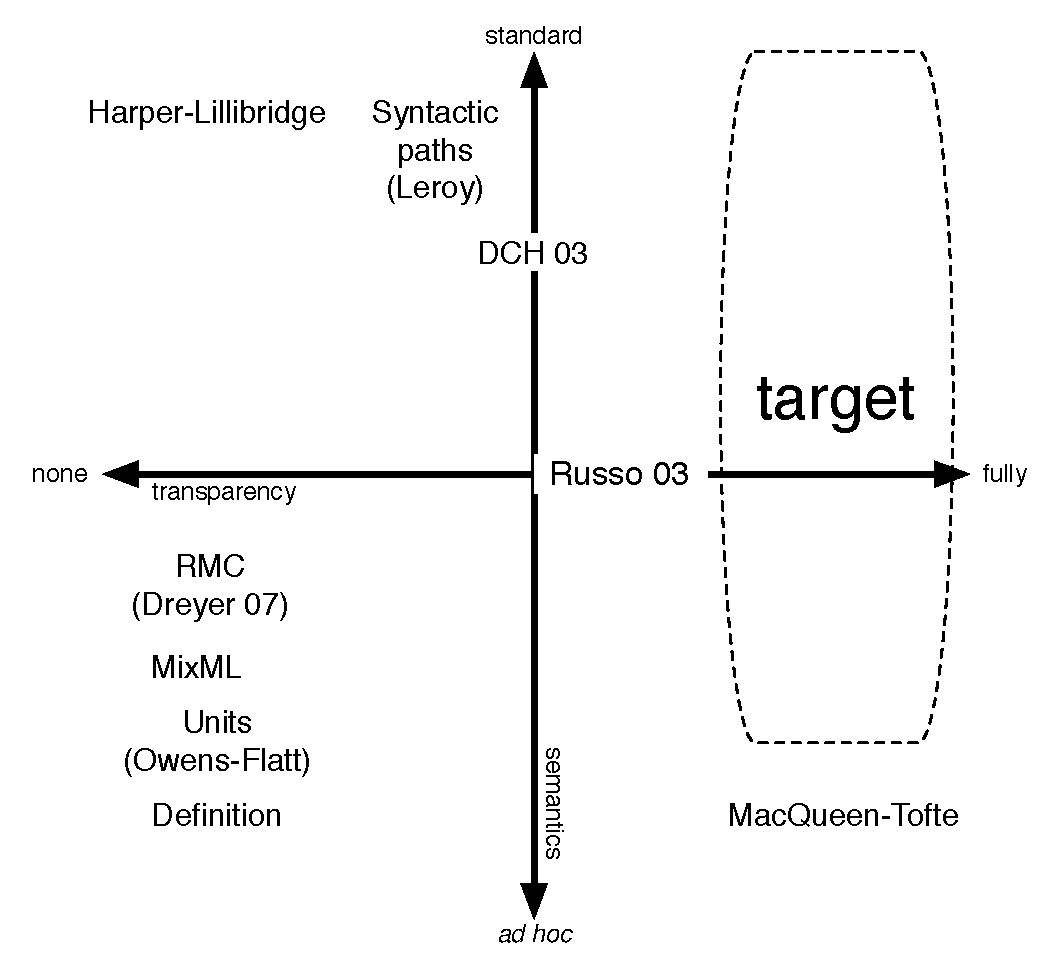
\includegraphics[scale=0.5]{../design/figs/modsys-spectrum.pdf}
\hrulefill\\
{\small A semantics is more standard in the sense that it uses more formal logic frameworks. It may potentially be easier to mechanize the metatheory of such semantics.}
\caption{The spectrum of major module system families}
\label{fig:spectrum}
\end{figure}

Besides the main module system features described earlier in this proposal, there are a number of other useful properties developed in the different module languages. The \emph{phase separation} \cite{hmm:phasedist} plays a fundamental role in ensuring that module systems can be typechecked fully at compile-time. This property is desirable, being consistent with our goal of static type safety. It says that a language, in this case a module, can be split into static and dynamic parts such that the static part does not depend on the dynamic. Some accounts of module systems respect phase distinction at the surface language level \cite{leroy95,russothesis}. Others respect the phase distinction in an internal language but not the surface language \cite{mt94}.  

The other key issue in a module system design is the existence of a \emph{principal signature} for modules. The term principal signature has been overloaded in meaning. Because of the many-to-many relationship between signatures and modules and the signature subtyping relationship, many signatures may be safely ascribed to a single structure. I will call the most precise signature for a structure (i.e., one that constrains all components of the structure with exact, most constraining types) the \emph{full signature}. A related concept is the \emph{free instantiation} of a functor formal parameter. The free instantiation is an instance of the functor formal parameter signature S that admits exactly enough type sharing to satisfy $S$ and no more. In particular, it avoids any extraneous type sharing that would cause potentially distinct types to be shared. What Dreyer \cite{dreyerthesis} calls the principal signature is the full signature in this terminology. Tofte defines principal signature of a signature expression $sigexp$ as one whose formal tycons can be instantiated to obtain all instantiations of $sigexp$ \cite{tofte92,mthm97}. I will adopt Tofte's terminology. 
   
\subsection{Syntactic Approach}
\subsubsection{CMU School}
Beginning with Harper-Lillibridge's translucent sums module calculus \cite{lillibridge94}, this large, prolific family of module systems pushed the state-of-the-art in terms of the type theoretic approach to module system design. Although Harper-Lillibridge originally explored first-class modules, the bulk of the research in this family was directed towards an applicative higher-order module semantics for type-directed compilers TIL/TILT and adding recursion. 

Crary \etal~\cite{crary99} and later Dreyer \cite{dreyer04,dreyer07} (DCH)
have explored adding support for recursion. Harper-Lillibridge
\cite{lillibridge94} and then Russo \cite{russo00} studied mechanisms
for making modules first-class entities in the core language. With
first-class modules, programmers can leverage the familiar module
system to take advantage of the System F-like power of the module
system for programming-in-the-small. Unfortunately, as Garcia
\cite{garcia05:extendedcomparing05} remarks, the syntactic overhead of
the ML module system makes this undesirable and impractical. When used
in a similar context, Garcia suggests that the type inference used for
type classes makes modular programming-in-the-small more
succinct. This observation holds only in the specialized case of type
classes. 

Harper and Stone \cite{harperstone} gave a semantics for ML modeling
every core language construct in terms of modules. This semantics was
based on the technique of using singleton signatures (and types) to
express type definitions \cite{stone00}. Dreyer's semantics uses a signature synthesis algorithm that
constructs a signature directly from a structure expression syntax
given the static environment as context. In
contrast, THO constructs a signature solely using the static environment. 

%Would this criterion apply to an example such as functor F() = struct datatype t end? 
%Why is making the distinction between generative and non-generative types at the individual spec level necessary? Wouldn't it be possible to emulate such behavior by lifting the individual type to a singleton module? 

%structure M = 
%struct
%  structure U :> sig type u end = struct type u = int end 
%   structure V :>> sig type v end = struct type v = bool end
% end

% using Dreyer's :>> weak sealing operator. 

\subsubsection{Syntactic Paths and Applicative Functors}
One of the first formal accounts of an ML-like module system is Leroy's manifest types calculus \cite{leroy94} where manifest types are definitional type specifications. The surface language for the manifest types calculus is equivalent to that of the translucent sums calculus described by Harper-Lillibridge\footnote{Definitional specs appeared in SML/NJ 0.93 a year before the Harper-Lillibridge paper appeared.}. The key observation in the manifest types calculus is that one can typecheck manifest types by comparing the rooted syntactic paths to those types which uniquely determine type identity. Thus, type equivalence is syntactic path equivalence for type constructors.  Leroy introduced the notion of applicative functors \cite{leroy95} which held types in the result of a functor application to be equivalent to corresponding types in all other results of applications of that functor to the ``same'' argument. Several designs \cite{shao99,dhc03,russothesis} have tried to incorporate both applicative and generative functors in a single calculus. Cregut \cite{CregutMacQueen94} enriched signatures with structure equalities to obtain complete syntactic signatures for separate compilation.

Leroy introduces a relatively simple approach to module system semantics that precludes shadowing of core and module bindings \cite{Leroy:generativity,leroy00}.
The semantics supports type generativity and SML90-style definitional sharing by reducing them to solving path equivalence by way of A-normalization (for functor applications) and S-normalization (a consolidation of sharing constraints by reordering). In his module system, Leroy claims that all type sharing can be rewritten in his calculus with generative datatypes and manifest types. However, Leroy's simplified module system does not include value specifications and datatype constructors both of which can constrain the order in which specifications must be written and therefore result in situations where sharing constraints cannot be in general reduced to manifest types. 

For full transparency, Leroy proved that there is a type-preserving encoding of a stratified calculus with strong sums without generativity using applicative functors\cite{leroy95}, claiming that the existence of such an encoding is a strong hint that applicative functors support full transparency. My HO apply functor example in fig.~\ref{fig:hoapplyfct} casts some doubt on this claim. As Leroy pointed out, under the strong sums model, first-class modules are at odds with phase distinction because of the typechecker would have to do arbitrary reductions\cite{leroy94}. In contrast, because the weak sum model of the manifest types calculus does not require any reductions at typecheck time regardless of the presence of first-class modules, it does not violate the phase distinction\cite{leroy94}. In the most recent paper in the manifest types series \cite{leroy00}, Leroy abstracts away most of the core language details from the manifest calculus to obtain a mostly core language independent module system. 

Although the syntactic paths approach may very well provide the simplest account of module systems, this is at the cost of some very fundamental shortcomings such as the inability to support shadowing and full transparency. Because the account's support for type sharing is incomplete, there may also be limits to how the semantics deals with the coherency issue. This dissertation will address these issues which are fundamental to the power of the ML module system. 

\subsubsection{Other ML Variants}
Shao \cite{shao:parameterizedsigsandho,shao99} defines a signature language based on gathering (and
internally factoring out) all flexible components (\ie, open 
specs unconstrained by sharing) in a higher-order type
constructor that can be applied to obtain a signature that expresses
functor body semantic actions at a later point. The resultant
signature language superficially resembles applicative
functors. However, type constructor applications in the signature
language must be on paths. Consequently, it does not support full
transparency in the general case. 

Govereau \cite{govereau:tr05} developed an alternative
semantics based on the type-theoretic approach. He claims that there
is no declaration that produces a generative type that is not
abstract, but datatype declarations could potentially be one of these
cases. One observation Govereau makes is that the static environment
must be ordered because types are dependent. Later bindings in the environment may refer to earlier bindings. The combination of applicative and generative types leads to a soundness problem similar to that found in Russo's Moscow ML system. 

The main contribution in Govereau's semantics appears to be a syntactic way to represent generativity that obviates the need for a Dreyer's effect system for managing the interaction between applicative and generative functors. The language uses distinct declarations for generative and non-generative abstract types. The type system declaratively partitions the static environment into two, corresponding to the lexical scope inside and outside a functor. 

The paper claims that if a type is defined ``under functor'' but does
not depend on a generative type defined under a functor, then it can
be coerced to non-generative. The claimed win is that although the syntactic purity judgment is not as fine-grain as DCH's effect system, it is simpler to work with. One disclosed limitation to both Govereau and Russo's systems is that a non-generative functor cannot have any generative types that are used in the body of the functor. 

Alice ML provides a number of the features mentioned in this chapter especially in the 
area of signature language enrichments. The language supports nesting signatures inside of signatures.
\begin{lstlisting} 
signature S = sig signature M = sig type t end end
\end{lstlisting}
Furthermore, the nested signatures can be left open to support signature-polymorphic functors.
\begin{lstlisting}
functor F (X:sig signature S structure Y : S end)  = ...
\end{lstlisting} 
The abstract signatures do not, however, appear to be complemented with any bounded polymorphism features. 

MLKit's semantics for elaboration calls for what amounts to defunctorization. In Elsman's view, functors are purely static constructs that can be compiled away, generating inlined copies of relevant dynamic content upon functor application. 
 
		Dreyer and Rossberg \cite{mixml} show how to encode ML signatures, structures, and functors in a mixin module calculus that appeals to something similar to Bracha's merge\cite{bracha:thesis} as its only linking mechanism. When linking a module A and B, the semantics tries to satisfy the imports of A using the exports of B and vice versa. The mixin merging syntax is {\bf link} x=M0 {\bf with} M1 in the surface language. It binds the name x to a module M0 and concatenates it with M1 merging components where appropriate. The scope of x is the body of M1. This mixin merging semantics supports recursion and separate compilation. Modules in this language consist of atomic modules that only contain values, types, type constructors, {\it etc}., labeled modules ($\{\ell = M\}$), and the merging form link ... with ....  

The peculiarity in this language is that modules and indeed anything that can be encoded in these modules are stateful. For example, signatures in MixML are fundamentally stateful. Linking against a signature S mutates it. Consequently, the typechecker rejects the following program. 
\begin{lstlisting}
module U = link x={module S = {type t}} 
           with {module A=(link x=x.S with {type t = int}), 
                 module b=(link x=x.S with {type t = bool})};		
\end{lstlisting}
Signatures must be suspended and then new'ed in order to be matched multiple times. This suspension is called a unit in Dreyer and Rossberg's terminology. Functors are also represented by suspending modules with unsatisfied imports. Although units have full support for hierarchical composition, MixML's design still retains the problem of stratifying modules and units, a problem inherited from the Flatt-Felleisen units that inspired it. 

	As it stands, the part of the MixML language that encodes the ML module system is but a small fraction of the whole. The question remains what implications the rest of the language has. Part of the language is obviously semantically meaningless such as {\bf link} X = [int] {\bf with} [3], which is a well-formed program. 

\subsubsection{Moscow ML}
Biswas gave a static semantics for a simpler form of higher-order modules \cite{biswas95}. The account relies on semantic objects and a stamp-based semantics similar to the Definition. The type propagation in higher-order functors is captured by a ``higher-order'' dependency variable that abstracted possible dependencies on the argument. These variables are only present in the internal language produced during elaboration. Consequently, Biswas's semantics does not support true separate compilation and neither does it enrich the surface syntax for signatures. Biswas's elaboration rule in fig.~\ref{fig:biswas-abstypespec-elab} maps an abstract type name t to the fresh higher-order abstract dependency variable $f$ applied to the list of all abstract dependency variables $\mathcal{W}$ it could possibly depend upon. For example, the functor parameter of the Apply functor, \lstinline{functor F(X:sig type t end): sig type t end}, is given the semantic representation $\forall f_0(\{t\mapsto f_0\} \Rightarrow \{t\mapsto f_1(f_0)\})$.

\begin{figure}
\hrule
~\\
\[
\infer {\Gamma,\mathcal{W}\vdash\mathrm{type~t}\Rightarrow ((t \mapsto f(\mathcal{W}), \emptyset), \{f\})}
{\textrm{$f$ is a fresh higher-order dependency variable}}
\]
$\Gamma$ is the type environment mapping program variables to types. $\mathcal{W}$ is a list of formal parameters variables the specification may depend on.
\hrule
\caption{Biswas's elaboration rule for abstract type specifications}
\label{fig:biswas-abstypespec-elab}
\end{figure}


Biswas's formal account was extended in a somewhat more type-theoretic
style to the full SML language and implemented by Russo in the Moscow
ML compiler \cite{russothesis}. One semantic
innovation was the use of existential types to represent abstract
types in a module system. The idea of using existential types
originated in a paper by Mitchell and
Plotkin~\cite{mitchellplotkin:popl85}. MacQueen pointed out how
scoping unpacks make conventional existential types ill-suited for
modular programming \cite{macqueen:popl86}. Montagu and R\'emy
\cite{Montagu-Remy:popl09:fzip} recently tried to address these
concerns by developing a variation of existential types which replaces
unpack with modular open and scope restriction constructs. 

Moscow ML also adds support for first-class
modules\cite{russo00} and a form of recursion \cite{russo01}. Moscow ML further attempts to incorporate both non-propagating
generative functors and applicative functors. The main limitation, as pointed out by Dreyer \cite{dreyerthesis}, is that Moscow ML's combination of generative and applicative functors is unsound. In particular, any generative functor can be $\eta$-expanded into an applicative functor thereby circumventing the generative functor abstraction. 

Russo notes the conflict between true separate compilation and
first-order module systems. He works around the problem by defining
compilation units to be only the sealed modules in an applicative
higher-order module system with first-order generative functors. To
address the avoidance problem, he introduces a hybrid name and
deBruijn-indexing scheme. 

Rossberg, Russo, and Dreyer \cite{tldi2010} developed a formal semantics based on a
translation to System F$_\omega$ enriched with records and existential
types in a recent variation on Russo's type system. In
this account, the type system of the module system was exactly the
type system of their variation on System F$_\omega$. All semantic
representations of signatures explicitly existentially quantified all
primary type constructors. The module system supported type
generativity insofar as existentials support it. The module system
does not claim to support full transparency, although there is an
extension of the system to support applicative functor semantics. 


\subsection{Units and Other Extralinguistic Linking Systems}
Flatt-Felleisen \cite{ff98} and Owens-Flatt \cite{owensflatt06} develop a module system semantics based on a calculus with stratified distinct hierarchically composable modules and recursively linkable units. Because both accounts appeal to extralinguistic linking semantics, they fall under the Module/Mesa line of module systems. As pointed out by Dreyer\cite{mixml}, the fundamental limitation in this semantics is that the stratification of units and modules precludes using unit linking and hierarchical composition together. One strength of their module system design is that it is one of the few accounts that includes an operational dynamic semantics, unlike all the other accounts discussed in this section. Some accounts of module systems give only a static semantics and perhaps a typechecking algorithm. Owens and Flatt prove type soundness of their semantics. 

Swasey \etal~\cite{swasey06} described a calculus SMLSC that is modeled after Cardelli's linkset approach to separate compilation. SMLSC introduces a compilation unit that sits on top of the module system that can be separately compiled from unimplemented dependencies by means of a handoff unit whose role resembles that of header files in C.

\subsection{The Definition and MacQueen-Tofte}
The module system semantics in the Definition of Standard ML \cite{mth90,mthm97} evolved throughout the late 1980s and early 1990s. Early on, Harper \etal~gave a fairly complete account of the static semantics of the first-order ML module system in terms of an operational stamp-based semantics \cite{hmt:tapsoft87}. Tofte in his thesis  \cite{toftethesis} proves that signature expressions in the first-order, generative semantics have principal signatures. He also extended this proof to cover non-propagating higher-order generative functors \cite{tofte:jfp94}. Then MacQueen and Tofte \cite{mt94} introduced true higher-order functor semantics. 

%Key to the semantics is the partitioning of structures into signature and {\bf realization} halves. A signature is the skeletal form of the structure, \ie, type and value specifications, with flexible type specifications that can be instantiated by signature matching. A realization fills in these flexible type specifications. 

Apart from type propagation transparency issues, the evolution of the Definition also addressed type sharing issues. The role of \emph{type sharing constraints} has evolved through the development of the Standard ML semantics and SML/NJ implementation. Type sharing constraints solve two problems in ML, type specification refinement and coherence. Originally, type specifications only declared the name of an expected type. It is quite useful to be able to refine type specifications to restrict them to particular definite types or by defining them relative to open specs. The \emph{coherence problem} is the challenge of constraining type components of two structures to be equivalent regardless of the actual identity of that type. In SML90 \cite{mth90}, explicit sharing equations among visible abstract type constructors and generative structure sharing were the sole means for constraining type specifications. Under generative structure sharing semantics, each structure had a unique static identity. Thus, two structures shared only when they were identical in the sense that they were defined at the same point in the program and are merely aliases (fig.~\ref{fig:structuresharing}). Under SML90 identity-based structure sharing, A and B have to be aliases, so the functor application at M4 fails to typecheck. Under SML97, the sharing constraint merely rewrites to sharing type A.t = B.t, thus both functor applications typecheck.
  Structures that shared in SML90 were equivalent both statically and dynamically. This kind of rich sharing semantics turned out to be quite complicated and was abandoned in favor of a structure sharing that implied type sharing constraints on congruent type specifications within the respective signatures. 

\begin{figure}
\begin{center}
\begin{tabular}{c}
\begin{lstlisting}
signature S0 = 
sig 
  type t
  val f : t -> t
  val state : t ref
end

functor F(X:sig 
           structure A : S0
           structure B : S0
           sharing A = B
          end) = ...

functor G() = 
struct
  type t = unit
  val f = ...
  val state = ref 0
end

structure M0 = G()
structure M1 = G()
structure M2 = M0

structure M3 = F(struct 
                structure A=M0
                structure B=M2
               end)

structure M4 = F(struct
                structure A=M0
                structure B=M1
               end)
\end{lstlisting}
\end{tabular}
\end{center}
\caption{SML90 structure sharing example}
\label{fig:structuresharing}
\end{figure}

SML/NJ 0.93 introduced definitional specifications, giving programmers two ways for constraining types to definite ones. SML97 added \lstinline{where type} and definitional type specifications completely replaced the definitional type sharing found in SML90. Definitional specifications and type sharing were finally disentangled. Generative structure sharing was eliminated in favor of the simpler semantics of a structural sharing that amounted to a type sharing equation for each common type component path, no matter how deeply nested. The semantics of type sharing and related mechanisms such as \lstinline{where type} are still somewhat problematical and unsettled \cite{narbel:jfp07,ramsey05}. Ramsey \etal~have argued that the scoping of \lstinline{where type} definitions should be more symmetric thereby permitting more flexible type specification refinements.

Shao \cite{shao98} (in a paper unrelated to the one on applicative functor-like module system \cite{shao99}) extends MacQueen-Tofte fully transparent modules with support for type definitions, type sharing (normalized into type definitions), and hidden module components. This treatment of higher-order modules is a more recent form of what is currently in the SML/NJ compiler. Elsman presents a module system compilation technique used in the ML Kit compiler \cite{elsman99}. The semantics follows the style of the Definition. The compilation technique is comparable to Shao's FLINT compilation scheme. 

The SML/NJ compiler implements a version of the module system that departs from the Definition in a number of aspects. Some of these extensions have not been formalized as of yet. In particular, the compiler has a richer semantics for \lstinline{include} and the elaborator compiles a functor body to a static lambda calculus which is what is used in place of the functor body re-elaboration at functor applications. The scoping of sharing constraints has also changed. In the current implementation, SML/NJ no longer permits nonlocal forms of sharing of the flavor illustrated in the example in MT (the first structure sharing constraint in fig.~\ref{fig:nonlocalsharing}). Both sides of the constraint must be in local scope as is in the second sharing constraint. Instead, structure definition specs express the same kind of sharing. For example, the structure definition spec \lstinline{structure A : sig end = S} expresses the first sharing constraint in SIG. The module system also has some significant limitations such as a lack of recursion, the tension between separate compilation and fully transparent generative functors, and weak facilities for signature composition.

\begin{figure}
\begin{center}
\begin{tabular}{c}
\begin{lstlisting}
structure S = struct type t end;
signature SIG = 
sig
  structure A : sig type t end
  structure B : sig type s end
  structure C : sig type s end
  sharing A = S
  sharing B = C
end	
\end{lstlisting}
\end{tabular}
\end{center}	
\caption{SML90-style structure sharing}
\label{fig:nonlocalsharing}
\end{figure}

\subsection{Type Generativity}

The idea of generative types has a significant history. More recently,
Neis~\emph{et al} \cite{neis:icfp09}, Dreyer and
Blume~\cite{dreyerblume:esop07}, Dreyer \cite{dreyer05}, and Rossberg
\cite{rossberg:ppdp03} have all developed semantics for studying type
generativity in the context of a System F$_\omega$-derived
language. Although the ML module system utilizes type generativity, it
only plays a role within the module system proper. After translation,
at which point the modules are eliminated, all the type generation has
already occured, having been carried out by the
elaborator. Consequently, the target language for translation, a
System F$_\omega$ language, need not contain any facilities for
generating fresh types. 

\subsection{First-class polymorphism inference and type classes}
	Jones \cite{jonesfcp} motivated first-class polymorphism (FCP) by appealing to the constructive logic tautologies for existentials, universals, and implication  \cite{jonesfcp}. The constructive logic rule $\langle w, \tau_w\rangle \rightarrow \tau' \leftrightarrow w \Rightarrow \tau_w \rightarrow \tau'$ corresponds to a translation of a module expression where types and values are coupled to System F$_\omega$ where types and values are decoupled (\emph{phase separation}) in the forward direction. More recent first-class polymorphic calculi such MLF \cite{Lebotlan-Remy/mlf-icfp} and FPH \cite{fph} add some limited type inference. Although inference in general may be undecidable, these limited inferencers still go a long way to make programming in these first-class polymorphic calculi more practical. If some of the ideas for inference for FCP calculi can be transferred over to a module calculus, one might also address the syntactic overhead of ML module systems. Adding FCP to the core introduces a certain amount of redundancy with respect to the FCP afforded by the module system. It would be useful to consider what exactly is redundant and whether that can be minimized. 
		
	Another language construct related to module systems that enjoys type inference is the type class. Type classes are a special case of modular programming where a kind of automatic deduction would be useful. Unfortunately, the scope of class instances are global. In Modular Type Classes, Dreyer \etal~ \cite{dhck07} develop semantics and a translation from type classes to a stylized use of the ML module system. 

\subsection{FLINT/Typed Cross Compilation}
The most closely related work is the formal semantics for a module
language called NRC given by
Shao~\cite{shao98}. Similar to this dissertation, NRC gives a formal semantics based on MacQueen-Tofte's
higher-order semantics. Unlike the present account, Shao's semantics
combines elaboration and translation into a single interweaving set of
judgments, whereas the present account cleanly separates them. The
separation of elaboration and translation is a conceptual
simplification and is also beneficial for more modular compiler
implementation. Also, Shao's semantics assumes a preprocessing step
that eliminates most of the interesting behavior involving coercive signature
matching. Although the NRC account alludes to the fact that the
functor body does not need to be re-elaborated at each application,
the NRC semantics does re-elaborate much like the MacQueen-Tofte
account. Finally, the NRC semantics does not directly support
datatype declarations, though it is claimed that it is a
straightforward extension. 

The account of NRC makes a few arguable
simplifying assumptions. Value components is a trivial extension that only requires a
  conversion of source-level types to semantic types. 
 Signature extraction is trivial only requiring the conversion of
  semantic types back to syntactic types. This conversion is
  guaranteed by the 1-to-1 mapping of the stamp environment. This is
  similar to our entity environment (see chapter~\ref{ch:entitycalc}), but as the semantics in 
  demonstrate, this is far from trivial.
 Shao says that value components in NRC are only elaborated once,
  but any type components may be re-elaborated. We simplify this even
  further. Only functor applications and type generation have to be
  re-elaborated. Type definitions can be expanded out early on during
  elaboration.
 As with some other accounts, NRC entangles type-checking and
  translation into F$_\omega$. Although translation clearly depends on
  type-checking, the converse case is not true. 
 In NRC, the assumption is that type-sharing constraints can all
  be converted to type definitions. As I have shown earlier, this is
  technically incorrect but probably practically adequate. 
 NRC requires A-normalization of the surface syntax SFC so that
  the only functor applications are of a functor variable (not
  paths) to a structure variable. In THO, the operator position of
  applications can be a path and the operand can be any structure
  expression. 
 The $\alpha$-renaming scheme described in NRC adds new
  declarations inside of existing structures in order to deal with
  signature ascription. 
 Signature matching is mostly handled during the SFC to NRC
  translation by adding explicit enrichment coercions. 
 NRC relies on a stamp environment, a finite map from stamp to
  tycon path. This has turned out to be unnecessary due to the
  existence of a function to perform the equivalent operation while
  relying on only the present semantics' structure entity itself. This function is the moral
  equivalent of an inversion of the realization although the
  realization does not technically admit an inversion. 


\subsection{Summary}
Not all module system designs enjoy the principal signature and phase distinction properties.  Fig.~\ref{fig:sys-features} summarizes the key features of the main ML-like module system families. Note that many module systems have various combinations of these features, but none are complete. Ideally, a module system would have true higher-order semantics and all the other features except for applicative functors which would be redundant. 

\begin{figure}
	\small
\begin{tabular}{|l|l|l|l|l|l|l|l|}
	\hline
System & higher-order & first-class & sep comp & rec & app & gen & phase\\
	\hline
	HL \cite{lillibridge94} & \ex & \chk & \chk & \ex & \ex & \ex & \chk \\
	\hline
	Leroy \cite{leroy95} & \ex & \ex & \chk & \ex & \chk & \ex & \chk \\
	\hline
	Russo \cite{russo01} & \ex & \chk & \chk & \chk & \chk & \chk & \chk \\
	\hline
	DCH \cite{dhc03} & \ex & \chk & \ex & \ex & \chk & \chk & \chk \\
	\hline
	RMC \cite{dreyer07} & \ex & \ex & \ex & \chk & \ex & \chk & \chk\\
	\hline
	%$\lambda^{\llparenthesis~\rrparenthesis}$ (\cite{ATTAPL}) & & & & & & \\
	%\hline
	%$\lambda^S$ (\cite{ATTAPL}) & & N & & N & N & N \\
	%\hline
	MT \cite{mt94} & \chk & \ex & \ex & \ex & \ex & \chk & \chk \\
	\hline
	MixML \cite{mixml} & \ex & \chk & \chk & \chk & \ex & \chk & \ex \\
	\hline
	Ideal & \chk & \chk & \chk & \chk & \ex & \chk & \chk \\
	\hline
\end{tabular}\\
higher-order = true higher-order\\
rec = recursive modules\\
app = applicative functors\\
gen = non-propagating generative functors\\
phase = respects the phase distinction
\caption{A comparison of major ML-like module systems}
\label{fig:sys-features}
\end{figure}		 										
 
%%% Local Variables: 
%%% mode: latex
%%% TeX-master: "main"
%%% End: 

	%!TEX root = main.tex

\chapter{The Design Space}\label{ch:designspace}

The simplest ML module system features only hierarchical composition of structures, type components in structures, transparent signature ascription, and first-order functors. Beyond this set of features lies a design space subject to debate. The module system design space is a rich one consisting of several functional dimensions. Much of the design space revolves around the module system's abstraction enforcement through opaque sealing and how that interacts with the other features of the module language. 

Dreyer frames the design space in terms of phase-separability and purity with respect to static and dynamic effects. In contrast, the goal of the THO semantics to focus on a simple framework for combining higher-order functors and type generativity. Type generativity is the central issue in the THO semantics. Although the semantics does not add anything new to the discussion of first-class and recursive modules, it appears that it neither complicates nor simplifies the issues concerning these two features.  


\section{Applicative Versus Generative Functor Semantics}
A chief point of contention is the support of applicative versus generative semantics for functors and the various attempts at supporting both. The central argument of applicative functor semantics is that a functor applied multiple times to the same path should produce results with the same type components. The original motivation was the support of higher-order functors with syntactic signatures. Subsequently, researchers have found few other examples where applicative functors have proven to be useful. One frequently cited example is the set functor (fig.~\ref{fig:setfunctor}). The claim is that one would want to apply the set functor multiple times to the same argument, opaquely ascribe each result, and still expect each result's corresponding types to be equivalent. 

\begin{figure}
\hrule
~
\begin{center}
\begin{tabular}{c}
\begin{lstlisting}
functor SetFn(K: sig type t ... end) = 
struct
  type set = K.t list
  val empty = [] 	
  fun isEmpty = ...
  ...
end :>
  sig 
     type set
     val empty : set
     val isEmpty : set -> bool
     ...
  end

structure IntKey = struct type t = int ... end
structure I0 = SetFn(IntKey)
structure I1 = SetFn(IntKey)

IO.isEmpty(I1.empty)
\end{lstlisting}
\end{tabular}
\end{center}
\hrule
\caption{Set functor}
\label{fig:setfunctor}
\end{figure}

\lstset{language=[Objective]caml}
\begin{figure}
\hrule
~
\begin{center}
\begin{tabular}{c}
\lstinputlisting{../apply-fct/ex4/fct.ml}
\end{tabular}
\end{center}
\hrule
\caption{fct.ml}
\label{fig:fctml}
\end{figure}

\begin{figure}
\hrule
\begin{center}
\begin{tabular}{c}
\lstinputlisting{../apply-fct/ex4/apply.ml}
\end{tabular}
\end{center}
\hrule
\caption{apply.ml }
\label{fig:apply1}
\end{figure}

Separating a functor F and the argument K into different files (figs.~\ref{fig:fctml} and~\ref{fig:apply1}), loading either of them more than once, and applying the functor will cause the types I.t and I0.t to be unequal under applicative semantics because they are either applications of the same syntactic functor to two different modules K (loading K twice gives rise to two different syntactic modules) or different syntactic functors to the same syntactic K.  

The above examples also come up in batch compilation. If both functor S and argument module K are defined in a compilation unit F (fig.~\ref{fig:fml}), then applicative semantics deems the client module in fig.~\ref{fig:apply2} well-typed.

\begin{figure}
\hrule
~
\begin{center}
\begin{tabular}{c}
  \lstinputlisting{../apply-fct/ex5/f.ml}
\end{tabular}
\end{center}
\hrule
\caption{f.ml}
\label{fig:fml}
\end{figure}

\begin{figure}
  \hrule
~
\begin{center}
\begin{tabular}{c}
	\lstinputlisting{../apply-fct/ex5/apply.ml}
\end{tabular}
\end{center}
\hrule
	\caption{apply.ml (batch compilation)}
        \label{fig:apply2}
\end{figure}

\lstset{language=ML}

Independently developed compilation units may each use an int set which is derived from independent applications of the generic set functor to an int key structure. The programmer might want these compilation units to exchange set values. Consider the example in fig.~\ref{fig:intkeyexample}. Unfortunately, applicative functors cannot help in this latter case. Because separate compilation loads the IntKey source twice, I0 and I1 are effectively applied to two different structures from a syntactic perspective. 

\begin{figure}
\hrule
~
\begin{center}
\begin{tabular}{l|l}
A & B \\
\begin{lstlisting}
structure IntKey = struct type t = int ... end
\end{lstlisting}

&
\begin{lstlisting}
structure IntKey = struct type t = int ... end
\end{lstlisting}
\\
\begin{lstlisting}
structure I0 = SetFn(IntKey)
\end{lstlisting} & 

\begin{lstlisting}
structure I1 = SetFn(IntKey)	
\end{lstlisting}
\end{tabular}
\end{center}
\hrule
\caption{Set functor separate compilation}
\label{fig:intkeyexample}
\end{figure}

Within a single compilation unit, the utility of applicative functor semantics seems questionable. If a functor has already been applied to an argument once, there is no need to apply it again. The result of the original functor application still exists and should be accessible. If the goal is to manage the namespace, then SML's semantics of structure abbreviations sharing types even opaquely ascribed ones is sufficient.  

Another problem with applicative functor semantics is that it is incompatible with type generativity. Consider the following example:

			\begin{lstlisting}
			functor F(functor G(X:T):T) = 
			struct 
			  datatype s = S of int 
			  structure M = G(struct type t = s end)
			  type u = M.t
			end	
			\end{lstlisting}

The semantics of datatypes is such that every application of F should produce a fresh tycon for s. The functor application of G depends on both the formal functor G and the fresh tycon s. The actual tycon s passed to the functor G is not known until F is applied, thus the dependency certainly cannot be expressed in terms of an applicative functor path. 

The other potential application is in distributed memory systems. Multiple computing nodes may each apply a functor to the same argument and then try to exchange values of a type in the result. Such a scenario will likely require runtime types. One argument in favor of applicative functors is in the construction of Okasaki's bootstrapped heaps \cite{okasaki}. However, even in that case, 

In OCaml, the syntax reflects the absence of generativity: there is no functor definition syntax that admits an empty parameter \lstinline{functor F() = ...}. Because the identity of functor body types depends on a syntactic parameter, each functor application must have one. Applicative functors are also incompatible with shadowing, a standard feature in functional languages. Because its notion of type equality is syntactic, OCaml does not support shadowing of type declarations in structures. For example, the following does not elaborate in OCaml:

\begin{lstlisting}
module M = struct type t = A type t = B val x = A end
\end{lstlisting}

\subsection{Generative Functors}\label{sec:ftgf}
There are implicitly two types of functors, those that have static effects, \emph{generative} functors, and those that do not, \emph{pure} functors. In the higher-order case, pure functors can be fully described using applicative functor-like syntactic extensions. The application of a functor to the same argument twice should give the same result because pure functor arguments are truly referentially transparent. This observation is certainly false when considering generative functors which have static effects. 

Type generativity is typically modeled using existential types. Each time an existential type is unpacked, a fresh abstract type is created. Dreyer, Crary, and Harper \cite{dhc03} advocated treating opaque sealing as a computational effect, a runtime fresh type generation. Dreyer \cite{dreyer05} reconciles this account of generative types with recursion via a backpatching type semantics. 

\subsubsection{Type Sharing}
Type sharing is necessary to support type-safe composition of modules. When a functor is parameterized over two modules which each declare an abstract type, the elaborator assumes that the two types are different. Consider the following example:

\begin{lstlisting}
signature S0 = sig
  type t 
  val a : t
end

signature S1 = sig
  type t
  val f : t -> int
end

functor F(structure X:S0 
	      structure Y:S1) = struct
  val y = Y.f(X.a)
end	
\end{lstlisting}

The above functor will not type check because there is no reason to believe \emph{a priori} that X.t and Y.t are equivalent. F can certainly be applied to X and Y such that X.t $\ne$ Y.t. If F is applied to X and Y such that X.t = Y.t, then this is an instance of the \emph{diamond import problem}. Simply put, when a single component, which may be a type or a structure, is exported in two different structures, it must be reconciled, retaining its identity and thus reflexive equivalence. The ML solution to this problem is type sharing. \emph{Type sharing} can be expressed in four forms. \lstinline{sharing type} constraints specifies equivalences on symbolic paths to types. The right hand side of \lstinline{sharing type} must consist of only symbolic paths to types. 

\begin{lstlisting}
functor F(structure X:S0
	      structure Y:S1
	      sharing type X.t = Y.t) = 
	...	
\end{lstlisting} 

\lstinline{where type}, which is derived from the categorical notion of fibrations, defines abstract type specs \emph{post hoc}. The left hand side of the \lstinline{where type} should be a signature S1 containing the type to be constrained. The right hand side consists of the name of the type t in S1 and an arbitrary type expression such as X.t or X.t list. 

\begin{lstlisting}
functor F(structure X:S0
	      structure Y:S1 where type t = X.t) = 
	...	
\end{lstlisting}

Definitional type specs constrains type specs inside of signatures. Consequently, they only apply if the signature is expanded out in the functor formal parameter. From the perspective of implementation, \lstinline{where type} elaborates to definitional type specs by pushing down the \lstinline{where type} definition to the relevant type spec. 

\begin{lstlisting}
functor F(structure X:S0
	      structure Y:sig 
	        type t = X.t
	        val f : t -> int
	      end) = ...	
\end{lstlisting}

The type sharing can also be expressed in terms of signatures parameterized on structures. This alternative was considered and rejected during the initial development of the ML module system in favor of \lstinline{where type} and \lstinline{sharing type} because parameterized signatures require programmers to anticipate all such sharing when writing the signatures. 

\begin{lstlisting}
signature S2(Z) = sig
  type t = Z.t
  val f : t -> int
end

functor F(structure X:S0
	      structure Y:S2(X)) = 
	...	
\end{lstlisting}

\section{First- Versus Second-Class Modules}
In most dialects of ML, the module system is second-class, meaning that there is a clear demarcation between the core and module languages. Module expressions cannot depend on the result of core language computations. Core language expressions can only access core language components in modules. They cannot operate on whole modules. This restriction is lifted in module systems with first-class modules, which in practice are useful for supporting plugins. The example for first-class modules often involve some runtime condition that determines the optimal abstract data structure to use, made available as modules, as illustrated by the example given by Dreyer~\cite{dreyerthesis}: 
~
\begin{lstlisting}
structure M = if n < 20 then LinkedList else HashTable	
\end{lstlisting}

The above is a kind of optimization that does not require first-class modules in their full generality. Neither, I would argue, does it fit with the main roles of a module system. Because the types in the structures LinkedList and HashTable may be completely different, the static description of M cannot be determined at compile-time. To avoid all the associated issues, language designers have often decided to limit first-class modules by requiring that such module expressions are opaquely ascribed to a single signature, an encoding which is a variation on existential types. Two proposals for first-class modules, Dreyer \cite{dreyerthesis} and Rossberg \cite{rossberg06}, take this approach. 

\begin{lstlisting}
structure M = if n < 20 then LinkedList else HashTable 
  :> sig type t type item val insert : t * item -> t ... end 	
\end{lstlisting}



\section{Recursive Modules}
In contrast to the triviality of mutual recursion in most programming languages, recursion at the module level is highly involved for module systems in statically-typed languages. Both the dynamic and static semantics are complicated by the static typing in the module system. Instead of the simple fixed point semantics for recursive module evaluation, the presence of type generativity necessitates alternatives because otherwise datatypes and opaque ascription will have generated new tycons for each recursive call. Even in the absence of datatype declarations and opaque ascriptions, ref cells and assignment in the core language are enough to complicate recursion at the module level. The standard work-around is to adopt Scheme's backpatching semantics except for the static part of the module. 

Backpatching semantics, however, must be made statically safe by ensuring that no recursive variable is used before it is backpatched. Furthermore, recursive modules should be amenable to separate compilation. Dreyer \cite{dreyerthesis} uses the concept of evaluability to enforce safety where a module is evaluable if it does not dereference an unbackpatched recursive variable. The characterization of evaluability is imprecise. The type system based on evaluability cannot determine the safety of some module expressions. 

The problem of type inference for recusive modules is complicated. In Dreyer's language, all recursive variables must be explicitly typed. Dreyer considers extending type inference to recursive variables, but this would require a complicated effect inference technique that produces large and complex types that possibly lack principality in the first place. 

%\subsection{Double Vision Problem}

\section{Signature Ascription}
Where the core language has type ascriptions, existing module systems support ascribing signatures to module expressions. Ascriptions are even more important in the module system than in the core language because module languages are explicitly typed and some forms of ascription serve as the primary means for enforcing data abstraction. 
 
Opaque ascription (\emph{i.e.}, sealing) should be construed as a deliberate design choice on the part of the programmer to make a type unique and incomparable. When using opaque ascription, the semantics should be simple. Alternative forms of opaque ascription such as the forms proposed by Dreyer \cite{dreyerthesis} and Govereau \cite{govereau:tr05} that make a type unique in some cases yet simultaneously comparable introduces a new set of issues that complicate the module system.    

\section{Separate Compilation}
Early module systems had two main guiding principles. First, modules should be partitioned into interface and implementation. The interface describes the form of a module, the implementation the details and mechanisms. Second, one should be able to compile modules independently from one another with only the aid of interfaces to resolve intermodule dependencies. In languages with simple type systems, reconciling these two goals is usually quite straightforward. 

The fundamental tension between separate compilation and an expressive, flexible module system is this: separate compilation requires the language to expose as much as possible in the interface or signature language but the goal of modularity is to keep a distinction between interface and implementation. Reconciling these two goals is a challenge in the ML language because of the presence of static effects. These effects, embodied in type generativity, are computed during the compiler elaboration process. Normally, a signature language should only contain information about the form of the module being described. Inclusion of static effect information would amount to adding information about the implementation. I contend that including static effects would run against the purpose of signatures. Moreover, it would entail significant code duplication and encourage further breakdown of the distinction between interface and implementation. 

As Russo~\cite{russothesis} noted because ML type information is spread between signature and realization, module clients that depend on the realization cannot be typechecked separately from the module. 

Normal ML syntactic signatures cannot even distinguish between functors that contain static effects and those that do not much less the nature of the static effect. For example, a functor body signature may contain a datatype declaration. Naively, an elaborator might consider this an indication that the functor body has a static effect, generating a fresh datatype upon each application. However, this assumption is incorrect because this specification matches both datatype replication declarations, which do not generate a fresh type,  \emph{bona fide} generative datatype declarations. 

\begin{lstlisting}
datatype t = K
structure M : sig datatype t = K end = 
struct
  datatype t = datatype t (* pure *)
end	
\end{lstlisting} 

Furthermore, the signature spec could have been \lstinline{type t} or \lstinline{datatype t = datatype t}. Consequently, an elaborator cannot handle the special case of pure functors by looking at the functor signature because they are indistinguishable from the signature. 

In order to support true separate compilation, the syntactic signature language must be extended with the entire entity calculus. The essence of the entity calculus is a small, simple language to express functor actions including type generativity. However, programming directly in the entity calculus would be an onerous task. One must account for all the potential functor actions when writing functor signatures. It would be much simpler to have the compiler produce entity expressions for describing functor actions as the elaboration semantics in the previous chapters has done. 

\subsection{Target Calculi and Type Sharing}
ML compilers often use enriched System F$_\omega$-like intermediate languages. Unlike the module system, System F$_\omega$ does not have any native support for type sharing. Naively compiling the type sharing example in sec.~\ref{sec:ftgf} produces $\Lambda t. \lambda a:t \Lambda s.\lambda f:s\rightarrow int. f(a)$, which is ill-typed. There are a number of solutions to this problem. 
\begin{enumerate}
\item Singleton kinds express the type sharing as a kinding of type $s$: $\Lambda.\lambda a:t.\Lambda s:\{t\}.\lambda f:s\rightarrow int.f(a)$. This technique is used in the TIL/TILT compilers and the Harper-Stone semantics. 
\item The $s$ dependency can be abstracted and expressed in terms of System F$_\omega$'s type constructors and expressions: $\lambda t.\lambda a:t.\lambda f:(\lambda s.s\rightarrow int)~t.f(a)$
\item FLINT preprocesses type sharing by replacing defined type names with their definitions: $\Lambda t.\lambda a:t.\lambda f:t \rightarrow int. f(a)$
\end{enumerate}

\subsection{Alternatives}
Despite its difficulty, true separate compilation is still desirable. As others have noted, one solution is to distinguish between compilation units and modules. Indeed, OCaml, Moscow ML, and Swasey's SMLSC take exactly this approach. In OCaml, each separate OCaml source file is a compilation unit which is a kind of quasi-module which must be coupled with an mli interface file. Because there is no compilation unit-level parameterization, the question of higher-order functors does not apply. Moscow ML only considers an opaquely seal module to be a compilation unit.    

\subsection{Relationship to Type Classes}
As Wehr notes, module encodings in terms of type classes also conflict with separate compilation. Because type classes are ordinarily transparent, they pose lead to type propagation problems similar to module systems.  

\subsection{Comparison to Shao}
Shao's calculus KMC aims to support both separate compilation and full transparency in higher-order modules by means of higher-order type constructors. The calculus is based on Harper-Lillibridge and Leroy's abstract approach, utilizing existentials for abstract types. The general idea is to factor out all the volatile components to a single higher-order type constructor. Inside of functor signatures, one can use selectors to project out the volatiles from this type constructor. Signatures are then parameterized by this higher-order type constructor. 

The Apply functor's signature would be $\lambda u_1:K.\Pi X:(\exists u_2.SIG[u_2]).(SIG[u_1[\overline{X}]])$. The higher-order type constructor $u_1$ plays a role similar to structure realizations and functor realization parameter. However, whereas structure realizations are completely distinct and nonoverlapping with signatures in M, the higher-order tycon is mixed in with syntactic signatures. This affords Shao's calculus the possibility of separate compilation.  

KMC's main limitation, however, is that it is still not flexible enough to express generative types and abstract types. Though KMC can model opaque sealing via existential types, it still cannot type check programs such as the following:

\begin{lstlisting}
signature SIG = sig type t val x : t end
funsig FSIG(X: SIG) = SIG

structure S = struct type t = int val x = 1 end

functor APPS (F:FSIG) = F(S)

functor G2(X: SIG) = 
struct 
  datatype t = A 
  val x = A
end
\end{lstlisting}

%\section{Entity Paths: Naming and Construction}
%\subsection{Related}
%\emph{Russo's hybrid deBruijn index}
%\emph{Harper-Lillibridge's internal names}
%%% Local Variables: 
%%% mode: latex
%%% TeX-master: "main"
%%% End: 

        
\chapter{Type System}\label{ch:typesystem}

\begin{figure}
\hrule

\[
\begin{array}{rcll}
p & ::= & x~|~p.x  & \textrm{symbolic paths}\\
K & ::= & \Omega~|~\Omega^n \Rightarrow \Omega & \textrm{kinds} \\
C^s & ::= & \alpha~|~p(\vec{C^s}) & \textrm{monotypes}\\
C^\lambda & ::= & \lambda\vec{\alpha}.C^s & \textrm{closed tycons}\\
T & ::= &
\mathsf{typ}(C^s)~|~\forall\vec{\alpha}.C^s & \textrm{closed types} \\
e & ::= & p~|~\lambda x.e~|~e_1 e_2 & \textrm{terms}
\end{array}
\]

\hrule
\caption{Surface type system}
\label{fig:typesystem}
\end{figure}


The syntactic type system consists of monotypes, type constructors (\emph{tycons}), and type expressions (\emph{aka} types). The monokind $\Omega$ and arrow kind $\Omega^n \Rightarrow \Omega$ classify monotypes and tycons respectively. As can be seen from the form of the arrow kind, the syntactic type system does not support higher-kinded tycons but it does support multi-arity tycons where the $n$ is a natural number indicating the arity of the tycon. Furthermore, the core language does not support impredicative polymorphism. Universal quantifiers for polymorphism are added in a semantic type system introduced later in this chapter. In the surface type language, the only type expressions that can occur on the right hand side of type definitions are type variables, arrow types, and type applications. Type functions are only introduced by the type definition construct in the core language. 

The kind and tycon language follow a significantly simplified version of Dreyer's language\cite{dreyerthesis}. The tycon language is an impredicative variant of System F$_\omega$ for simplicity, although the core language does not take advantage of impredicativity because the tycon expressions are an elaborated version of the core language types, which do not contain universal quantifiers at all since the quantifiers are added at the module declaration level. Type expressions ($T$) classify core language terms.  Monotypes may be of two forms. Type variables ($\alpha$) come from a denumerable set. The tycon application form ($p(\vv{C^s})$) requires the type operator to named by the symbolic path $p$. By letting the argument of the application be an empty vector, the form can represent all simple types as an application of a nullary type operator to an empty argument vector. 

Wrapping an $n$-ary $\lambda$-abstraction around a monotype produces a tycon. 
The $\lambda$ tycon denotes type functions parameterized by tycon variables $\vec{\alpha}$. The vector of tycon parameters may be empty thus permitting nullary type functions, which represent nullary tycons. 

In the syntactic tycon language, $\lambda$-abstractions are $n$-ary and not curried, so applications must be saturated. Using the $\lambda$-abstraction to represent even nullary tycons ensures that the semantics can distinguish definitional tycons, \emph{i.e.}, they are exactly those wrapped with an outer $\lambda$-abstraction. $C^\lambda$ are the only syntactic tycons, but semantic tycons, described in sec.~\ref{sec:semtypesys}, add forms corresponding to datatype tycons. This does not reduce the expressiveness of the tycon language at all. In fact, it is a very close match to the tycon language in ML, considerably closer than more general languages found in previous treatments. 

 The universal type expression ($\forall\vec{\alpha}.C^s$) represents polymorphism. Universal quantifiers only occur at the structure declaration level.

\section{Kind System}\label{sec:typesystem-kindsystem}
%!TEX root = ../main.tex

\begin{figure}
\hrule

\[\begin{array}{rcll}
Path & = & \textrm{set of all symbolic paths}\\
Tyc_{syn} & = & \textrm{set of all closed syntactic tycons}\\
\Delta & ::= &\emptyset_{knds}~|~\Delta[\alpha] & \textrm{kind environment}\\
\Gamma & : & Path \rightharpoonup Tyc_{syn} & \textrm{static environment}
 \end{array}
\]

\fbox{$\Gamma,\Delta\vdash C^s : \Omega$}

\begin{equation}
\infer{\Gamma,\Delta \vdash \alpha : \Omega}{\alpha \in \Delta}
\label{eq:syntypevar}
\end{equation}

\begin{equation}
\infer{\Gamma,\Delta \vdash p(\vec{C^s}) : \Omega}
{\Gamma, \Delta \vdash
  \Gamma(p) :  \Omega^n \Rightarrow \Omega
  \qquad |\vec{C^s}| = n \qquad \Gamma,\Delta\vdash C^s_i : \Omega
  ~\forall i\in [1,n]}
\label{eq:syntypeapp}
\end{equation}

\fbox{$\Gamma,\Delta\vdash C^\lambda : \Omega^n \to \Omega$}

\begin{equation}
\infer{\Gamma,\Delta \vdash \lambda\vec{\alpha}.C^s :
  \Omega^n\Rightarrow \Omega}{\Gamma,\Delta
  [\alpha_1]\ldots[\alpha_n] \vdash C^s : \Omega}
\label{eq:syntypelam}
\end{equation}

\fbox{$\Gamma\vdash T : \Omega$}

\begin{equation}
\infer{\Gamma\vdash \mathsf{typ}(C^s) : \Omega}{\Gamma,\emptyset_{knds} \vdash
  C^s : \Omega}
\label{eq:syntypeinj}
\end{equation}

\begin{equation}
\infer{\Gamma \vdash \forall\vec{\alpha}.C^s :
  \Omega}{\Gamma,[\alpha_1]\ldots[\alpha_n]
  \vdash C^s : \Omega}
\label{eq:syntypeforall}
\end{equation}

\hrule
\caption{Well-kinding of syntactic tycons}
\label{fig:kindingsyntactic}
\end{figure}
     

The well-kinding judgments (Fig.~\ref{fig:kindingsyntactic}) are of the form $\Gamma,\Delta\vdash C : K$
where $C$ is $C^s, C^\lambda,$ and $T$. The static environment
$\Gamma$ is used to interpret symbolic paths in monotype application
forms $p(\vv{C^s})$. At this point, one can think of $\Gamma$ as a
finite partial map from symbolic paths to syntactic tycons. In chapter~\ref{ch:homods}, static environments will be formally defined. $\Gamma(p)$ calculates a tycon, either a defined tycon or a tycon produced by datatype declaration, which is internal, accessible by a type variable. $\Delta$s represent the kind environment, which contains all the bound type variables, which by default have kind $\Omega$. Again, only monokinds are necessary here because the syntactic type system does not support higher-kinded tycons. Also noteworthy is that type variables $\alpha$ can only be of the monokind (rule~\ref{eq:syntypevar}). 

The tycon application kinding rule (\ref{eq:syntypeapp}) checks that the operator tycon path is well-kinded, the correct number of arguments is supplied and that each of the arguments is well-kinded with kind $\Omega$. The notation $C^s_i$ denotes the $i$th element in the $\vv{C^s}$ vector. The rest of the rules ensure that the types and tycons are closed with respect to type variables (\ie, all type variables are in $\Delta$). 

\section{Semantic Type System}\label{sec:semtypesys}

\begin{figure}
\centering
\small
\hrule
\[
\begin{array}{rcll}
    \tau^n & \in & \mathrm{Tycs} & n\textrm{ is arity}: \Omega^n\Rightarrow \Omega\\
\\
    \mathfrak{C}^s & ::= & \alpha~|~\mathfrak{C}^\lambda(\vv{\mathfrak{C}^s}) & \textrm{semantic monotype}\\
    \mathfrak{C}^\lambda & ::= &
    \lambda\vec{\alpha}.\mathfrak{C}^s~|~\tau^n & \textrm{semantic tycon}\\
    \mathfrak{T} & ::= &
    \mathsf{typ}(\mathfrak{C}^s)~|~\forall\vec{\alpha}.\mathfrak{C}^s
    & \textrm{semantic type expression}\\
    \mathfrak{C}^{nf} & ::= &
    \alpha~|~\tau^n(\vv{\mathfrak{C}^{nf}}) & \textrm{normal form monotypes}\\
% Why both the C^s and \lambda forms? Is the C^s form necessary at
% this point? 
\end{array}
\]
\hrule
\caption{Semantic type system}
\label{fig:semtypesystem}
\end{figure}

The foregoing type system is purely syntactic. There is no semantics for evaluating the type expressions and tycons. Syntactic types cannot be evaluated directly due to the presence of the uninterpreted symbolic paths. Fig.~\ref{fig:semtypesystem} gives a \emph{semantic} type language that replaces the symbolic paths in the tycon application form with tycons. Semantic monotypes, tycons, and type expressions are distinguished from their syntactic counterparts by the Fraktur script ($\mathfrak{C}$). The semantic type language is first-order and simply-kinded.The Tycs set is the set of all tycon symbols $\tau^n$, distinct from syntactic symbols. Each such tycon has an assigned arity $n$. The elements in Tycs will be called \emph{atomic tycons}.  All primitive tycons such as int, bool, and arrow fall into the Tycs set and all generated datatype tycons will be elements of Tycs. 

The semantic type system consists of semantic monotypes ($\mathfrak{C}^s$), semantic tycons ($\mathfrak{C}^\lambda$), and semantic type expressions ($\mathfrak{T}$) each of which corresponds to the respective syntactic type system version. Semantic monotypes differ from syntactic monotypes in that semantic tycons replace symbolic paths in the application form. Semantic tycons consist of both a $\lambda$ form that represents definitional tycons and a $\tau^n$ form, a concrete, atomic tycon from Tycs, which is intended to represent tycons generated by datatype declarations, opaque ascription, and functor applications. The arity of well-formed tycons can always be calculated directly, $|\tau^n| = n$ and $|\lambda\vec{\alpha}.\mathfrak{C}^s|$. 

\begin{figure}
\hrule

\fbox{$\Delta\vdash \mathfrak{C}^s : \Omega$}

\begin{equation}
\infer{\Delta \vdash \alpha : \Omega}{\alpha \in \Delta}
\label{eq:semtypevar}
\end{equation}

\begin{equation}
\infer{\Delta \vdash \mathfrak{C}^\lambda(\vec{\mathfrak{C}^s}) : \Omega}
{\Delta \vdash
  \mathfrak{C}^\lambda :  \Omega^n \Rightarrow \Omega
  \qquad |\vec{\mathfrak{C}^s}| = n \qquad \Delta\vdash \mathfrak{C}^s_i : \Omega
  ~\forall i\in [1,n]}
\label{eq:semtypeapp}
\end{equation}

\fbox{$\vdash \mathfrak{C}^\lambda : \Omega^n \to \Omega$} 

\begin{equation}
\infer{\vdash \lambda\vec{\alpha}.\mathfrak{C}^s :
  \Omega^n\to \Omega}
{
  [\alpha_1]\ldots[\alpha_n] \vdash \mathfrak{C}^s : \Omega}
\end{equation}

\begin{equation}
\infer{\vdash \tau^n : \Omega^n \to \Omega}
{\strut}
\label{eq:semtypeatomic}
\end{equation}

\fbox{$\vdash \mathfrak{T} : \Omega$} 

\begin{equation}
\infer{\vdash \mathsf{typ}(\mathfrak{C}^s) : \Omega}
{\emptyset_{knds} \vdash  \mathfrak{C}^s : \Omega}
\label{eq:semtype-typ}
\end{equation}

\begin{equation}
\infer{ \vdash \forall\vec{\alpha}.\mathfrak{C}^s :
  \Omega}
{[\alpha_1]\ldots[\alpha_n]
  \vdash \mathfrak{C}^s : \Omega}
\label{eq:semtype-fa}
\end{equation}

\hrule
\caption{Well-kinding of semantic tycons}
\label{fig:kindingsemantic}
\end{figure}


Fig.~\ref{fig:kindingsemantic} gives a kind system for semantic monotypes, tycons, and type expressions. This kind system differs from the the previous one in fig.~\ref{fig:kindingsyntactic} in that the application rule~\ref{eq:semtypeapp} no longer needs to look up a static environment for a symbolic path, because there are no symbolic paths. The simplifies the kind system in that the static environment can be dropped. To handle atomic tycons, the kind system also adds rule~\ref{eq:semtypeatomic} that gives it the arrow kind $\Omega^n\Rightarrow\Omega$ to match its arity. Thus, the role of this kind system is solely to verify that arities match up and that the types are closed with respect to type variables.  

\subsection{Notation}\label{sec:typesystem-notation}
Let $\mathfrak{C}^\lambda$ be a semantic tycon. $|\mathfrak{C}^\lambda|$ refers to the arity of the tycon. If the tycon is an atomic tycon $\tau^n$, then $|\tau^n|=n$. If the tycon is a $\lambda\vec{\alpha}.\mathfrak{C}^s$, then the arity is the length of the $\vec{\alpha}$. The $|\cdot|$ notation is also carried over in the obvious way to relativized tycons. $\mathfrak{C}^{nf}_1 \equiv_\alpha \mathfrak{C}^{nf}_2$ is the equivalence of two semantic monotypes module $\alpha$-renaming of type variables,\ie~the two monotypes are isomorphic up to $\alpha$-renaming of type variables. 

\subsection{Evaluation}
Semantic type expressions and monotypes can be evaluated by a $\beta$-reduction rule in Fig.~\ref{fig:semtyceval} to a normal form $\mathfrak{C}^{nf}$. Note that the normal form of atomic tycons with 0-arity is $\tau^0()$. 


\begin{figure}
\centering
\hrule 
\small
\setlength{\tabcolsep}{0ex}
\renewcommand{\arraystretch}{1.1}
~\\[1mm]
\begin{equation}
\infer{(\lambda\vec{\alpha}.\mathfrak{C}^s)(\vv{\mathfrak{C}^s}) \Downarrow_{mt} \mathfrak{C}^{nf}_2}
{\vv{\mathfrak{C}^s}\Downarrow_{mt} \vv{\mathfrak{C}^{nf}_1}\qquad\mathfrak{C}^s\{\vv{\mathfrak{C}^{nf}_1}/\vec{\alpha}\} \Downarrow_{mt} \mathfrak{C}^{nf}_2} 
\end{equation}
\hrule
\caption{Semantic tycon evaluation}
\label{fig:semtyceval}
\end{figure}

The evaluation rule is the typical big-step call-by-value $\beta$-reduction modified to accept a vector of arguments. Since the semantic type language is analogous to a simply-typed $\lambda$-calculus (actually a first-order simply-typed $\lambda$-calculus enriched with constants), the language is strongly normalizing (lem.~\ref{lem:tycred}). 

\begin{lemma}[Monotypes are strongly normalizing]
If $\mathfrak{C}^s \Downarrow_{mt} \mathfrak{C}^s_1$ and $\mathfrak{C}^s \Downarrow_{mt} \mathfrak{C}^s_2$, then $\mathfrak{C}^s_1 = \mathfrak{C}^s_2$ and $\mathfrak{C}^s_1$ is a $\mathfrak{C}^{nf}$. 
\end{lemma}

Not only are the types strongly-normalizing, the semantic type language also has preservation and progress properties. 

\begin{lemma}[Kind Preservation]
If $\emptyset_{knds}\vdash\mathfrak{C}^s:\Omega$ and $\mathfrak{C}^s \Downarrow_{mt} \mathfrak{C}^{nf}$, then $\emptyset_{knds}\vdash\mathfrak{C}^{nf} : \Omega$. 
\end{lemma}
 
\begin{lemma}[Progress]
If $\emptyset_{knds}\vdash\mathfrak{C}^s:\Omega$, then $\mathfrak{C}^s \Downarrow_{mt} \mathfrak{C}^{nf}$. 
\end{lemma}

The connection between the syntactic and semantic type systems will be made clear in chapter~\ref{ch:homods}.  

%%% Local Variables: 
%%% mode: latex
%%% TeX-master: "main"
%%% End: 

        \chapter{Surface Language}\label{ch:surfacelang}
%!TEX root = ../main.tex

\begin{figure}
\hrule
\[
\begin{array}{lrcl}
\textrm{Core declarations} & d^c & ::= & \mathsf{val}~
x=e~|~\mathsf{type}~t=C^\lambda~|~\mathsf{datatype}~\vec{\alpha}~t\\
        & spec & ::= & \mathsf{structure}~x :
        sigexp~|~\mathsf{type}~\vec{\alpha}~t\\
        & & ~~| & \mathsf{type}~t = C^\lambda\\ 
	& & ~~| & \mathsf{functor}~f(x:sigexp_1) : sigexp_2\\
        & & ~~| & \mathsf{val}~x:T\\
        & specs & ::= & \emptyset_{specs}~|~spec, specs\\
	& sigexp & ::= &
        x~|~\mathsf{sig}~spec~\mathsf{end}~|~sigexp~\mathsf{where~
          type}~p=C^\lambda\\
%        & & ~~| & sigexp~\mathsf{where}~p_1=p_2\\
	& strexp & ::= & p~|~\mathsf{struct} ~d^m~\mathsf{end}
        ~|~p(strexp)\\
        & & ~~| & strexp:sigexp~|~strexp:>sigexp\\
\textrm{Module decls}	& d^m & ::= & \circ~|~\mathsf{structure}~x = strexp,
d^m\\
       & & ~~| & \mathsf{functor}
       ~f(x:sigexp)=strexp, d^m~|~d^c, d^m\\
\textrm{Top level decls} & d^t & ::= & \circ~|~\mathbf{signature}~x=sigexp,d^t~|~d^m,d^t

\end{array}
\]
\hrule
\caption{Surface module language}
\label{fig:modlang}
\end{figure}



\section{Core Language}

The surface language (Fig.~\ref{fig:modlang}) closely follows SML/NJ's syntax with a few exceptions. There are three forms of core level declarations: value, type definition, and datatype. For type definitions, the type parameters are written in an explicit $\lambda$-abstraction form $\mathsf{type}~t = \lambda\vec{\alpha}.C^s$ instead of $\mathsf{type}~\vec{\alpha}~t=C^s$. Definitional type specs use a similar notation. For simplicity, the data constructor part of datatype declarations is omitted. The interesting behavior is the datatype declaration's generation of a fresh atomic tycon.

The core language is a simple one comprised of an implicitly typed expression language ($e$) and a simple declaration language ($d^c$). There are three forms of declarations in the core language, value declarations, type definitions, and datatype declaration. For simplicity's sake, datatype declarations only declare the name and parameters (arity) of a generative tycon. 

\section{Signatures} 
A signature is a tree of static information for a structure. This object is a hierarchy because it must reflect the hierarchical nesting of structures. The hierarchy can be considered a tree where the internal nodes are structure specifications (\emph{i.e.}, a signature for a named structure) and the leaves are static entities for tycons and functors. 

Signatures are defined as a sequence of comma separated specs. Value specs use the notation $\mathsf{val}~x:\forall\vec{\alpha}.C^s$ instead of $\mathsf{val}~\vec{\alpha}~x=C^s$. Each sequence is terminated by the empty spec $\emptyset_{specs}$. Signature expressions include a variable form, base signature $\mathsf{sig}~spec~\mathsf{end}$, and a signature expression modified by a where type clause. Signature declarations are always at top level.

In signatures, there are two kinds of tycon specifications, definitional and open. \emph{Definitional tycon specs} (abbreviated as \emph{definitional specs}) constrain tycons that can be matched. \emph{Open tycon specs} (abbreviated as \emph{open specs}) only declare the name and arity of a tycon that must be present in a matching structure.

\begin{singlespace}
\begin{lstlisting}
type ('a, 'b) s = 'a list * 'b (* definitional *)
type ('a,'b) t                      (* open *)
\end{lstlisting}
\end{singlespace}

Definitional specs are intended to match type definitions in structures. Open specs can match type definitions, datatype declarations, and abstract types (\ie, a type component made abstract by opaque ascription) in structures. 

Signature expressions may be the base form that contains specs. The where type form of signature expressions is a generalization of SML's mechanisms. The where type form adds the type definitions on the right hand side to the structure spec (signature expression) identified on the left hand side. 

Since signature expressions support the base form of signatures and these expressions are found in signature specs, module declarations, and top level declarations, this amounts to the possibility of inline base signatures throughout the language. The presence of inline signatures must be accounted for during elaboration. 

%The mechanism subsumes the structure definition spec form found in SML. Structure definition specs, which have the form \lstinline{sig structure M : sig ... end = A end} where A is a previously defined structure, can be encoded as \lstinline{sig structure M : sig ... end end where M = A}. These special forms of signature expressions will be discussed further in a later section. 

\section{Module Calculus}

Structure expressions can be a path $p$, a base structure, a functor
application (where the functor occurs only as a symbolic path $p$),
transparent signature ascription, and opaque signature ascription. A
module declaration is a sequence of structure, functor, and core
declarations. $\circ$ denotes the empty structure declaration that
terminates every sequence of structure declarations. At the top level,
in addition to module declarations, one may also have signature
declarations. The top level declaration sequence is terminated by an
empty top level declaration $\circ$. 

The semantics of transparent and opaque ascription follow that of Standard ML. Unlike some of the more recent module systems, Standard ML's signature ascription is always a coercion on the structure to the form specified in the signature. In the transparent case, this amounts to dropping any value bindings or type declarations omitted in the signature. However, when a signature's open spec is matched against a structure's type definition, the resulting coerced structure will reveal that type definition. In the opaque case, this kind of type definitions is occluded. 

\section{Primary and Secondary Components}\label{sec:primaries}
The form of a functor argument is constrained by the functor parameter signature possibly modified by a where type definition. In the parameter signature, there can be structure specifications, formal functor specifications, structure/type sharing constraints, and the two classes of type specifications. The open and definitional specs in functor formal parameter signatures are worth special mention. The tycon names declared by these specs may occur in the functor body. When typechecking these occurrences, a free instantiation (\ie, dummy instantiation) of the tycon is used. SML/NJ also supports a rich notion of symmetric type sharing constraints, that will be deferred for future work. Where type constraints can turn open specs into definitional ones when pushed down. Open specs that remain open specs after the resolution of all sharing and where type constraints correspond to these free instantiations. These free instantiations are called \emph{formal} tycons. These are exactly the flexible tycons mentioned in Shao~\cite{shao98}. 

In the presence of type sharing constraints, which induce an equivalence class of formal tycons, each equivalence class has a canonical representative called a \emph{primary} tycon. Without type sharing constraints, all formal tycons are primary.
These primary tycons are the essential components that must be kept to maintain the semantics of functor application (\ie, the type application associated with the functor application). References to all other members of the equivalence class should be redirected to the associated primary type component. The remaining type components (from definitional specs) are \emph{secondary} and therefore should be fully derivable from the primary tycons and externally defined types. Secondary types do not have to be explicitly represented in the parameter signature because all occurrences of these secondary types can be expanded out according to their definitions. 

\begin{lstlisting}
functor F(X:sig type s type t type u = s * t sharing type t = s end) = ...
\end{lstlisting}

	In the above example, \lstinline{s} can be primary, representative for the equivalence class containing both \lstinline{s} and \lstinline{t}, and \lstinline{u} is secondary. Primary tycons are the ones that must be instantiated each time a functor is applied. The primary tycons must then be substituted into the secondary tycons or, alternatively, looked up in an environment described in chapter~\ref{ch:entitycalc}. 
 
\section{Nonvolatile and Volatile Type Constructors}\label{sec:volatile}
In the module system, tycons can be classified as either nonvolatile or volatile. \emph{Nonvolatile tycons} are atomic tycons in the initial static and entity environments. Open type specs in signatures, datatype declarations, and tycons defined relative to former two give rise to \emph{volatile tycons},{\it i.e.}, they may be instantiated to a particular tycon by functor application or signature matching. Moreover, volatile tycons can be instantiated multiple times through different functor applications or signature matching. Although volatile tycons overlap with the notion of abstract types, they are not the same. The defining characteristic of volatile tycons is that their actual instantiation will be supplied at a later point and they can have multiple instantiations within a program. The instantiation used changes depending on the context, thus the tycon is volatile. In cases such as transparent signature ascription, a volatile tycon may be perfectly transparent. 

Volatile types themselves can be classified as primary (open tycon specs in functor formal parameters and signatures) and secondary (tycons defined relative to primary volatile tycons). 

\begin{lstlisting}
functor F(X: sig
      type a (* primary, volatile *)
      type b = int (* secondary, nonvolatile *)
      structure M0 : 
      sig
         type c (* primary, volatile *)
         type d = a (* secondary, volatile *)
      end
      end) =
  struct
     type u = X.a list (* secondary, volatile *)
     structure M1 : 
        sig 
           type v (* spec, not a tycon *)
        end = struct
        type v = X.M0.c * int (* secondary, volatile *)
     end
  end
\end{lstlisting}

The above example illustrates some of the complexities of volatile types. Types X.a and X.M0.c are obviously volatile. Definitional types X.M0.d, u, and M1.v are also volatile because they are defined in terms of volatile types. 

%%% Local Variables: 
%%% mode: latex
%%% TeX-master: "main"
%%% End: 
  
        \chapter{Entity Calculus}\label{ch:entitycalc} 
In this module system, I will use an entity calculus, a refined
version of the static representation of functor actions and static
module content found in the SML/NJ compiler. The entity calculus
provides a natural representation of the static content of modules,
which I call \emph{static entities}. The term entity refers to an
extended\footnote{Entity calculus tycons differ from syntactic types
  only in that the tycons may have been relativized, a process
  described in a later section, and prefixed polymorphic (universal) quantifiers.}
form of type constructors ($\mathbb{C}^\lambda$) and a static
description of objects that may include type constructors such as
structures and functors. In the module system, syntactic signatures
alone are insufficient for expressing functor actions. The entity
calculus is a small language for expression exactly that, the functor
actions for a functor. 
   
\input{../design/figs/fig-rlzn}
   
Fig.~\ref{fig:entities} describes the entity calculus, comprising of
entity expressions $\varphi$, entity declarations $\eta$, and static
entities $\upsilon$. The static entities are the entity calculus
analogue to values in the lambda calculus. The representation relies
on a denumerable set of variables, EntityVars, which represents unique names that can be thought of as the new variable names resulting from alpha-conversion.
  
Entity environments $\Upsilon$ are sequences of bindings of an entity
variable $\rho$ to a static entity $\upsilon$. The sequence is
important because the semantics needs a deterministic way to search
through the environment for atomic tycons. The role of entity environments is two-fold. They give the
current instantiation of a relativized tycon, thus enabling
translation of a relativized tycon to a specific semantic
tycon. Furthermore, they permit the translation of a semantic tycon
back to an entity path, a canonical relativized tycon. 
     
There are four forms of static entities, corresponding to structure, functor, atomic tycons, and definitional
(derived) tycons. Structure and functor entities are enclosed in
$\langle\rangle$ brackets. A structure entity
$\langle\Upsilon^{lcl},\Upsilon^{clo} \rangle$ has a
local entity environment $\Upsilon^{lcl}$ and a closure environment
$\Upsilon^{clo}$ to close an associated semantic signature with respect to any entity variable not defined in $\Upsilon^{lcl}$, \ie, the nonlocal entity variables. 

\begin{lstlisting}
signature S = 
sig
  type t
  structure S' = sig val x : t end
end

structure M =
struct
  type t = int
  structure S ' = struct val x = 1 end
end
\end{lstlisting}

Consider the above example. The semantic signature S' has a free occurrence of the entity variable for t $\rho_t$. The entity variable $\rho_t$ is not in the domain of the entity environment for S'. In fact, the entity environment for S' is empty because S' does not contain any static entities. Still, the structure entity for S' must be self-contained. Therefore it must close the signature for S' with a closure entity environment which is a copy of the entity environment for its enclosing structure.  A structure entity encodes only the volatile type information in structure, \ie, the part that is re-instantiated with signature matching and functor application. 

There are two forms of functor entity. The standard form
$\langle\lambda\rho.\varphi;\Upsilon\rangle$ encodes the functor
action as an \emph{entity function} $\lambda\rho.\varphi$ together with a closure
entity environment $\Upsilon$. Applying an entity function results in a structure entity. The alternate form
$\langle\lambda\rho.\Sigma;\Upsilon\rangle$ 
represent functors in formal functor parameters where the
only information known is the semantic signature $\Sigma$ of the functor result, described in chapter~\ref{ch:homods} in fig.~\ref{fig:semanticobjs}. Semantic signatures
are syntactic signatures where each of the static
components (tycons, structures, and functors) are decorated with
entity variables. They are formally defined in chapter~\ref{ch:homods}. A semantic signature may mention entities by their entity variables (called \emph{relativized} tycons), hence it must closed by an entity environment $\Upsilon$. Relativization is formally defined in sec.~\ref{sec:relativization}. Atomic tycons
$\tau^n$ and definitional tycons $\mathfrak{C}^\lambda$
(defined in sec.~\ref{sec:relativized-type-sys}) are
the tycon entities. Entity environments may contain definitional tycons because of signature matching, a subject thoroughly discussed in sec.~\ref{sec:sigmatch}. 

Static entities are the values computed by the entity calculus. Tycon entity expressions evaluate to tycon entities. Previously declared tycons and formal tycons from functor parameters are represented by their entity path, $\vec{\rho}$. They can also be a $\newx(n)$ or a relativized tycon $\mathbb{C}^\lambda$ (defined in sec.~\ref{sec:relativization}) that refers to a tycon whose instantiation is in an entity environment. The $\newx(n)$ form produces a new atomic tycon $\tau^n$ when evaluated where $n$ specifies the arity of the desired tycon. The $\newx(n)$ expression is the key to representing type generativity in the entity calculus. Datatypes and other generative tycons are represented by the form $\newx(n)$ which when evaluated will generate a fresh type constructor unequal to all those generated before it. 

Structure entity expressions and functor entity expressions evaluate to
structure entities and functor entities respectively. The entity path
form in both structure and functor entity expressions is a reference
to an entity bound in a previous entity declaration. Structure entity
expressions also consist of entity declarations enclosed by
$\llparenthesis\cdot\rrparenthesis$ corresponding to the
\lstinline{struct ... end} base structure form, functor application expressions, and 
let expressions. The let expression is used to express coercions induced by
signature matching (see sec.~\ref{sec:sigmatch}). In addition to an
entity path, functor entity expressions may be entity lambda abstractions or 
formal functors of the form $\lambda\rho.\Sigma$. 
 
Entity declarations bind an entity variable to tycon entity expressions, structure entity
expressions, and functor entity expressions. The entity calculus has a static compile-time semantics. The elaborator evaluates entity expressions to static entities as necessary during elaboration. The judgments for the entity expression evaluation are outlined below:
 
\begin{tabular}{ll}
	$\Upsilon\vdash\varphi \Downarrow_{str} R$ & structure entity expression evaluation \\
	$\Upsilon\vdash\eta \Downarrow_{decl} \Upsilon'$ & entity declaration evaluation \\
	$\Upsilon\vdash\theta \Downarrow_{fct} \psi$ & functor entity expression evaluation
\end{tabular}

$\Upsilon$ is an entity environment. $\varphi$ is the resulting entity expression.  $\psi$ is a resulting functor entity. $R$ is the entity environment obtained by evaluating the structure entity expression. $\Upsilon'$ is the entity environment obtained by evaluating the entity declarations $\eta$. Each binding in $\Upsilon'$ corresponds to an entity declaration in $\eta$, thus $\Upsilon\not\subseteq\Upsilon'$. 

\section{Entity declarations}
The evaluation rules for entity declarations must accumulate the entity environment across declarations in order to support occurrences of entities in value specs within inline open signatures. 

\begin{singlespace}
\begin{lstlisting}
datatype d = A

structure M : sig type t val x : d * t end =
struct
  datatype t = B
  val x = (A, B)
end
\end{lstlisting}
\end{singlespace}

Observe that the type name d is a nonlocal name that must be defined in a prior entity declaration. The clause entity environment for M must contain a binding for d.  

\section{Notation}\label{sec:entitycalc-notation}
I indicate extension of entity environments by juxtaposition, $\Upsilon[\rho\mapsto\upsilon]$. This notation should never cause shadowing of entity variable bindings because the convention is that $\rho\notin dom(\Upsilon)$. 
Entity environment concatenation of two entity environments $\Upsilon$ and $\Upsilon'$ is represented by juxtaposition, $\Upsilon\Upsilon'$. The notation for entity environment lookup is overloaded. $\Upsilon(\rho)$ looks up the static entity corresponding to $\rho$. The notation $\Upsilon(\rho_0\vec{\rho})$ looks up $\rho_0$ in $\Upsilon$ for a structure entity $R=\langle \Upsilon^{lcl},\Upsilon^{clo} \rangle$ and then recursively computes $\Upsilon'(\vec{\rho})$ such that $\Upsilon' = \Upsilon^{clo}\Upsilon^{lcl}$. Let $EV(\cdot)$ denote the set of all entity variables in $\cdot$. The notation $dom(\Upsilon)$ denotes the set of entity variables in the domain of all mappings in $\Upsilon$, including the nested ones. 

Let $R$ be a structure entity $\langle\Upsilon^{lcl},\Upsilon^{clo}\rangle$ and $\vec{\rho}$ be an entity path defined in either $\Upsilon^{lcl}$ or $\Upsilon^{clo}$. Then $R(\vec{\rho})$ is defined such that $R(\vec{\rho}) = \Upsilon^{clo}\Upsilon^{lcl}(\vec{\rho})$. 

$\Upsilon_1 \subseteq \Upsilon_2$ indicates all the bindings in
$\Upsilon_1$ are in $\Upsilon_2$. The notation $R \subseteq \Upsilon$
means $\Upsilon^{clo}\Upsilon^{lcl}\subseteq \Upsilon$ where $R=\langle
\Upsilon^{lcl}, \Upsilon^{clo}\rangle$. Similarly, $\Upsilon\subseteq R$
indicates $\Upsilon \subseteq \Upsilon^{clo}\Upsilon^{lcl}$. The convention that that if $R$ is used in a place where an entity environment is expected, then $R$ denotes $\Upsilon^{clo}\Upsilon^{lcl}$ such that $R = \langle \Upsilon^{lcl}, \Upsilon^{clo} \rangle$. 

\section{Entity Evaluation Semantics}
\input{../design/figs/fig-evalent}

Entity declarations evaluate to entity environments. The module system evaluates entity expressions when elaborating functor application (rule \ref{eq:strapp}). Each entity expression represents the latent static computation in a structure or functor expression. Once evaluated, the resultant structure entity provides a precise and complete (closed) description of the entities inside a structure. Evaluation requires an entity environment as context to interpret entity paths in the entity expressions and declarations. 

Fig.~\ref{fig:entsems} lists the rules for evaluating entity expressions. The key rules are the ones for application (\ref{eq:expapp}). There are two, one for regular functor application and the other for formal functor application. The functor entity expression is evaluated to an entity function. The argument structure entity expression is evaluated to an entity environment. The body of the entity function is then evaluated in an entity environment extended with the closure environment and the formal parameter entity variable mapped to the argument structure entity environment. Rule~\ref{eq:expappformal} evaluates the functor entity expression to a functor entity corresponding to the formal functor case and also the structure entity expression to the structure entity. The semantic signature $\Sigma$ (\ie~the formal functor body signature) must be instantiated (a process that is covered in sec.~\ref{sec:siginst}). The rule then forms a structure entity using this instantiation and the extended entity environment as a closure. The instantiation part of the closure will correspond to the actual functor closure when the actual functor is known. 

%!TEX root = ../principles.tex
\begin{figure}
\centering

\fixedCodeFrame{
\small
~\\[0.5mm]
\fbox{$\Upsilon\vdash \eta \Downarrow_{decl} \Upsilon'$}
\begin{equation}
	\infer{\Upsilon\vdash\bullet\Downarrow_{decl} \emptyset_{ee}}
        {\strut}
\label{eq:entdecempty}
\end{equation}

\begin{equation}
	 \infer{\Upsilon\vdash\rho=_{str}\varphi,\eta\Downarrow_{decl}[\rho\mapsto R]\Upsilon'}
	{\Upsilon\vdash\varphi\Downarrow_{str}R\qquad 
          \Upsilon[\rho\mapsto R]\vdash\eta\Downarrow_{decl}
          \Upsilon'} 
\label{eq:entdecstr}
\end{equation}
	
\begin{equation}
	\infer{\Upsilon\vdash\rho=_{fct}\theta,\eta\Downarrow_{decl}[\rho\mapsto\psi]\Upsilon'}
	  {\Upsilon\vdash\theta\Downarrow_{fct}\psi\qquad 
            \Upsilon[\rho\mapsto\psi]\vdash\eta\Downarrow_{decl}
            \Upsilon'}
\label{eq:entdecfct}
\end{equation}

\begin{equation}
	\infer{\Upsilon\vdash\rho=_{tyc}\newx(n),\eta\Downarrow_{decl}
          [\rho\mapsto\tau^n]\Upsilon'}
	    {\begin{array}{c}
                \Upsilon[\rho\mapsto\tau^n]\vdash\eta\Downarrow_{decl}\Upsilon'\qquad
            (\tau\textrm{ is fresh in }\Upsilon)
          \end{array}} 
\label{eq:entdecnew}
\end{equation}

\begin{equation}
         \infer{\Upsilon\vdash[\rho=_{def}\mathbb{C}^\lambda],\eta\Downarrow_{decl}
           [\rho\mapsto\mathbb{C}^\lambda]\Upsilon'}
         {\Upsilon[\rho\mapsto\mathbb{C}^\lambda]\vdash\eta\Downarrow_{decl}
           \Upsilon'}
         \label{eq:entdectypedef}
\end{equation}

\begin{equation}
         \infer{\Upsilon\vdash[\rho=_{def}\vec{\rho}],\eta\Downarrow_{decl}
           [\rho\mapsto\Upsilon(\vec{\rho})]\Upsilon'}
         {\Upsilon[\rho\mapsto\Upsilon(\vec{\rho})]\vdash \eta
           \Downarrow_{decl} \Upsilon'}
         \label{eq:entdecalias}
\end{equation}
}
\caption{Entity declaration semantics}
\label{fig:entdecsems}
\end{figure}
Entity declarations must be evaluated in
sequence. Fig.~\ref{fig:entdecsems} formally defines how to evaluate
entity declarations. Each tycon, structure, and functor entity declaration evaluates the respective tycon, structure entity expression, and functor entity expression to the corresponding entity. The subsequent entity declarations are evaluated in the context of an entity environment extended with a mapping for that entity. The entity environment context only has bindings for the entity variables bound in the entity declarations because only entity expression evaluation will provide the correct closure.

Rule~\ref{eq:entdecempty} ensures that the resultant entity
environment is cumulative. Rules~\ref{eq:entdecstr}
and~\ref{eq:entdecfct} evaluate structure and functor entity
declarations in the expected way.  Rule~\ref{eq:entdecnew} is the key
rule that generates fresh atomic tycons with the appropriate arity
$n$. When the $\rho=_{tyc}\newx(n)$ entity declaration is embedded in
the body of a functor entity, it produces a fresh atomic tycon for
$\rho$ each time the functor entity is applied,\ie~also when this
entity declaration is evaluated. This models exactly the behavior of
generative datatype declarations under true higher-order
semantics. Rule~\ref{eq:entdectypedef} yields a corresponding type
definition entity environment binding. Rule~\ref{eq:entdecalias} looks
up an entity path (constructed during signature matching coercion
rule~\ref{eq:coerceopen}) for the corresponding entity mapping. 
  
%!TEX root = ../principles.tex
\begin{figure}
\centering
\fixedCodeFrame{
\small
~\\[2mm]
\fbox{$\Upsilon\vdash\theta\Downarrow_{fct}\psi$}
\begin{equation}
\infer{\Upsilon\vdash\vec{\rho}\Downarrow_{fct}\Upsilon(\vec{\rho})}
{\strut} 
\label{eq:fctentpath}
\end{equation}

\begin{equation}
\infer{\Upsilon\vdash\lambda\rho.\varphi
\Downarrow_{fct}\langle
  \lambda\rho.\varphi;\Upsilon\rangle}
{\strut}	
\label{eq:fctentlam}
\end{equation}

\begin{equation}
\infer{\Upsilon\vdash\lambda\rho.\Sigma \Downarrow_{fct} \langle
  \lambda\rho.\Sigma; \Upsilon
  \rangle}
{\strut}
\label{eq:fctentformal}
\end{equation}

}
\caption{Functor entity evaluation}
\label{fig:fctenteval}
\end{figure}
 
Fig.~\ref{fig:fctenteval} gives the rules for evaluating a functor entity expression. Rule~\ref{eq:fctentpath} looks up entity paths in the usual way. The entity function is formed by combining an entity $\lambda$-abstraction with the current entity environment to form a closure (rule~\ref{eq:fctentlam}). Rule~\ref{eq:fctentformal} similarly forms a closure for formal functors.  

\begin{lemma}[Entity evaluation terminates]
The following evaluation relations terminate (have a finite derivation tree):
\begin{enumerate}
\item $\Upsilon\vdash\varphi\Downarrow_{str}R$
\item $\Upsilon\vdash\eta\Downarrow_{decl}\Upsilon'$
\item $\Upsilon\vdash\theta\Downarrow_{fct} \psi$
\end{enumerate}
\end{lemma}

\begin{lemma}
\begin{enumerate}
\item If $\Upsilon \vdash \varphi \Downarrow_{str} R$, then
$\Upsilon\subseteq R$.
\item If $\Upsilon\vdash \theta \Downarrow_{fct}
\langle\theta;\Upsilon'\rangle$, then $\Upsilon\subseteq\Upsilon'$. 
\end{enumerate}
\end{lemma}

\section{Relativization}\label{sec:relativization}
Tycon names have a scoping policy much like other program identifiers. Tycon names can be shadowed by later tycon declarations. A tycon name may refer to a local tycon that is declared in the same semantic signature or structure entity, or to a nonlocal one that is declared as a functor parameter or in another structure. Although signature declarations occur only at the top level, anonymous signature expressions may be embedded as functor parameter signatures and signature ascriptions. When signatures occur inline, its type specifications may refer to both local and nonlocal tycons.

Some tycon names may refer to volatile tycons which may be instantiated multiple times possibly to new generative tycon. Each time a functor is applied or a structure is ascribed a signature, the tycon name must be interpreted according to a potentially different entity environment. When elaboration reaches these tycons we need a way to map them back to the corresponding entity path such that we reference the correct ``up-to-date'' volatile tycon. The necessity of this is illustrated in fig.~\ref{fig:lifecycle}. Semantic tycons which live in static environments and entity environments have to be relativized when put into semantic signatures and entity expressions. When the tycon is needed for typechecking, the tycon must be instantiated with respect to an entity environment. This is the primary purpose of relativization, to give an entity path that can be interpreted according to different entity environments. Secondarily, relativization replaces fragile symbolic names with robust entity paths to the entity environment mapping the entity paths. 

\begin{figure}
\begin{center}
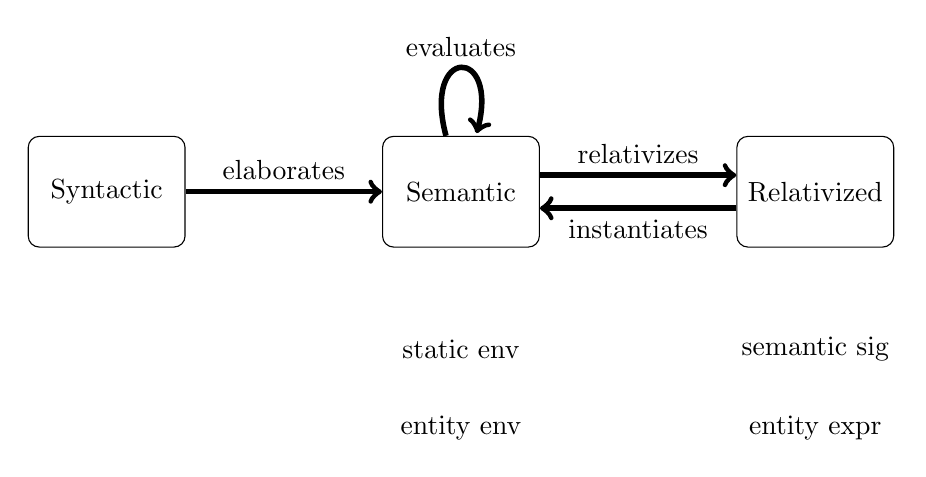
\begin{tikzpicture}[node distance= 4.5cm,auto]
\tikzstyle{block} = [rectangle, draw,  
    text width=5em, text centered, rounded corners, minimum height=4em]
\tikzstyle{arr} = [line width=2pt,->]
	\node[block] (sy) {Syntactic};
	\node[block, right of=sy] (se) {Semantic};
	\node[block, right of=se] (re) {Relativized};

	\node[node distance=2cm,below of=se] (statenv) {static env};
	\node[node distance=1cm,,below of=statenv] {entity env};
	\node[node distance=2cm,below of=re] (semsig) {semantic sig};
	\node[node distance=1cm,below of=semsig]  {entity expr};
		
	\path[arr] (sy) edge node {elaborates} (se);
	\path[arr] ([yshift=-5mm]se.north east) edge node {relativizes} ([yshift=-5mm]re.north west);
	\path[arr] (se) edge [loop above] node {evaluates} (se);
	\path[arr] ([yshift=5mm]re.south west) edge node {instantiates} ([yshift=5mm]se.south east);
	

\end{tikzpicture}
\end{center}
\caption{Life-cycle of a tycon}
\label{fig:lifecycle}
\end{figure}

\subsection{Relativized Type System}\label{sec:relativized-type-sys}
\begin{figure}
	\hrule
\[\begin{array}{rcll}
       \mathbb{C}^s & ::= &
         \alpha~|~\vec{\rho}(\vv{\mathbb{C}^s}) & \textrm{relativized monotypes}\\
       \mathbb{C}^\lambda & ::= & \lambda\vec{\alpha}.\mathbb{C}^s &
       \textrm{relativized tycons}\\

        \mathbb{T} & ::= &
        \mathsf{typ}(\mathbb{C}^s)~|~\forall\vec{\alpha}.\mathbb{C}^s & \textrm{relativized type expression}\\

\end{array}\]
\hrule
\caption{Relativized type system}
\label{fig:reltypesystem}
\end{figure}

  
The relativized type system ($\mathbb{C}^s, \mathbb{C}^\lambda,$ and $\mathbb{T}$) replaces all occurrences of atomic tycons with entity paths. The purpose of relativization and this type system is described in section~\ref{sec:volatile}. Three classes of tycons have been introduced: syntactic, semantic, and relativized. The semantics progressively translates syntactic tycons to the latter two. The module system only evaluates semantic tycons. Such tycons exist in the static and entity environments. In contrast, relativized tycons are never reduced directly. Instead, they must be instantiated into a semantic tycon for reduction to take place as in fig.~\ref{fig:lifecycle}. Relativized tycons exist in semantic signatures and static environment by way of embedded semantic signatures. 


\begin{figure}
\hrule

\begin{equation}
\infer{\Upsilon, \Delta \vdash \alpha :: \Omega}
{\alpha \in \Delta}
\label{eq:r-k-var}
\end{equation}

\begin{equation}
\infer{\Upsilon, \Delta \vdash \vec{\rho}(\vv{\mathbb{C}^s}) :: \Omega}
{\Upsilon, \Delta \vdash \Upsilon(\vec{\rho}) :: \Omega^n \to \Omega\qquad
 \Upsilon, \Delta \vdash \mathbb{C}^s_i~\forall \mathbb{C}^s_i \in \vv{\mathbb{C}^s}}
\label{eq:r-k-app}
\end{equation}

\begin{equation}
\infer{\Upsilon \vdash \lambda\vec{\alpha}.\mathbb{C}^s 
:: \Omega^n \to \Omega}
{n=|\vec{\alpha}|\qquad\alpha_i\in\vec{\alpha}~i\in[1,n]\qquad
\Upsilon, [\alpha_1]\ldots[\alpha_n] \vdash \mathbb{C}^s :: \Omega}
\label{eq:r-k-abs}
\end{equation}

\begin{equation}
\infer{\Upsilon\vdash\mathsf{typ}(\mathbb{C}^s) :: \Omega}
{\Upsilon,\emptyset_{knd}\vdash \mathbb{C}^s :: \Omega}
\label{eq:r-k-typ}
\end{equation}

\begin{equation}
\infer{\Upsilon\vdash \forall\vec{\alpha}.\mathbb{C}^s :: \Omega}
{n=|\vec{\alpha}|\qquad\alpha_i\in\vec{\alpha}~i\in[1,n]\qquad \Upsilon,[\alpha_1]\ldots[\alpha_n]\vdash \mathbb{C}^s :: \Omega}
\label{eq:r-k-fa}
\end{equation}

\hrule 

\caption{Well-kinding of relativized monotypes, tycons, and types}
\label{fig:relativized-wellkinding}
\end{figure}




Relativized monotypes, tycons, and types must also be well-kinded as
defined in Fig.~\ref{fig:relativized-wellkinding}. The main difference
between this well-kinding judgment and the other well-kinding
judgments is that rule~\ref{eq:r-k-app} uses the entity environment to
obtain a well-kinded {\bf semantic} tycon. The rest of the semantics
is standard. 
 

\begin{figure}
\centering
\small
\fixedCodeFrame{
~\\[0.5mm]
\begin{equation}
\infer{\Upsilon\vdash \mathbb{C}^s_1 \equiv \mathbb{C}^s_2}
{\Upsilon(\mathbb{C}^s_1) \Downarrow_{mt} \mathfrak{C}^{nf}_1\qquad
  \Upsilon(\mathbb{C}^s_2) \Downarrow_{mt} \mathfrak{C}^{nf}_2\qquad
  \mathfrak{C}^{nf}_1 \equiv_\alpha \mathfrak{C}^{nf}_2 }
\label{eq:mtequiv}
\end{equation}

\begin{equation}
\infer{\Upsilon\vdash \lambda\vec{\alpha}.\mathbb{C}^s_1 \equiv \lambda\vec{\beta}.\mathbb{C}^s_2}
{\begin{array}{c}
|\vec{\alpha}|=|\vec{\beta}|\qquad \Upsilon\vdash \mathbb{C}^s_1
\equiv \{\vec{\alpha}/\vec{\beta}\}\mathbb{C}^s_2 
\end{array}}
\label{eq:tcequiv}
\end{equation}
}
\caption{Monotype and tycon equivalence}
\label{fig:mt-tyc-equiv}
\end{figure}

\begin{figure}
\centering
\small
\fixedCodeFrame{
~\\[0.5mm]
\fbox{$\Upsilon\vdash \mathbb{T}_1 \equiv \mathbb{T}_2$}

\begin{equation}
\infer{\Upsilon\vdash \mathsf{typ}(\mathbb{C}^s_1) 
  \equiv \mathsf{typ}(\mathbb{C}^s_2)}
{\Upsilon\vdash \mathbb{C}^s_1 \equiv \mathbb{C}^s_2}
\label{eq:teequiv-typ}
\end{equation}

\begin{equation}
\infer{\Upsilon\vdash \forall\vec{\alpha}.\mathbb{C}^s_1 
  \equiv \forall\vec{\beta}.\mathbb{C}^s_2}
{|\vec{\alpha}|=|\vec{\beta}|\qquad\Upsilon\vdash\mathbb{C}^s_1 \equiv
\{\vec{\alpha}/\vec{\beta}\}\mathbb{C}^s_2}
\label{eq:teequiv-forall}
\end{equation}
}
\caption{Type expression equivalence}
\label{fig:typeequiv}
\end{figure}



The rules in Figs.~\ref{fig:mt-tyc-equiv} and~\ref{fig:typeequiv}
define monotype and tycon equivalences and type expressions
equivalences respectively.   
The module system semantics will require a notion of relativized monotype equivalence and relativized tycon equivalence, which are given by rules~\ref{eq:mtequiv} and~\ref{eq:tcequiv} respectively.  Monotypes and tycons are equivalent under the interpretation of an entity environment when they evaluate to equivalent normal form semantic tycons modulo $\alpha$-renaming. Rules~\ref{eq:teequiv-typ} and~\ref{eq:teequiv-forall} describe equivalence for type expressions. 

\subsection{Role of Relativization}
Relativization plays in a role in signature extraction (discussed in sec.~\ref{sec:sigextract}):
\begin{enumerate}
\item Value bindings in the static environment must be relativized. 
\item Definitional type binding in the static environment must be relativized in the inferred signature. 
\end{enumerate}
        
\begin{lstlisting}
sig
  structure M : sig type t end
  type u = M.t 
end
\end{lstlisting}

\noindent The type definition for u must be relativized because it refers not to a concrete type, but a type defined relative to a matching structure's realization.

Consider the following example:
\begin{lstlisting}
structure A =
struct
  structure B = struct datatype u end
  functor F(X:sig type t end) = 
    struct val a : X.t * B.u = ... end : sig val a : X.t * B.u end
end
\end{lstlisting}

The following are the semantic signatures for the example:
\[B \mapsto (\rho_B, \{u \mapsto (\rho_u, 0)\})\]
\[X \mapsto (\rho_X, \{t \mapsto (\rho_t, 0)\})\]
In the type for a, the tycon for X.t must be relativized to $\rho_X\rho_t$ and for B.u to $\rho_B\rho_u$. 

When inferring the signature from the body of F, we have the formal tycon X.t in the static environment. When inferring the signature from F's body, there are two static environments, the static environment produced by elaborating F's body and the contextual static environment when entering into the body. 

Static environment for F's body: $[a \mapsto \tau_t^0 * \tau_u^0 ]$ \\
Static environment for the context: $[B \mapsto (\rho_B, \{u \mapsto (\rho_u, \tau_u^0)\}, R_B)]$\\
                 $[X \mapsto (\rho_X, {t \mapsto (\rho_t, \tau_t^0)}, R_X)]$

$R_B$ and $R_X$ are the structure entities for $B$ and $X$ respectively. 


\begin{lstlisting}
structure A =
struct [$\rho_A$]
  structure B = struct [$\rho_B$] datatype t [$\rho_t$] = K end
  functor F(X [$\rho_X$]:sig type u [$\rho_u$] val a : u end) =
  struct 
    val b : X.u * B.t = (X.a, B.K)
  end : sig val b : X.u * B.t end
end
\end{lstlisting}

The relativized tycon, an entity path, can be computed from the static environment at the point of elaboration. For example, when the elaborator reaches the body of the above functor, the static environment is the following:

$[B\mapsto (\rho_B, \langle \{t \mapsto (\rho_t, 0)\}, \emptyset_{ee}\rangle)][X\mapsto (\rho_X,\langle\{u\mapsto(\rho_u,0), a\mapsto [\rho_u]\},\emptyset_{ee}\rangle)]$

The tycon for \lstinline{X.u} can be relativized by building an entity path, \emph{i.e.}, $\rho_X\rho_u$, by traversing the static environment. 

When elaborating the specified type of \lstinline{a} in the functor parameter signature, the reference to the formal tycon \lstinline{u} is relativized to an entity path $\rho_u$. 

After instantiation of the parameter signature during functor elaboration (sec.~\ref{sec:modelab}),  the elaborator must derive the canonical entity path for any newly generated tycons, structures, and functors, which will correspond to an entity variable in the parameter signature. The elaborator uses the canonical entity path when elaborating the functor result signature and functor body. 

This after-the-fact entity to entity path mapping is also needed for structure bindings to create the mappings for coerced entities produced during signature matching. Unlike in the functor case, mappings for the entities in the structure binding and the structure entity itself must be in scope for the rest of the program. 

A policy of fully reducing a tycon before relativizing 
simplifies the process of relativization. Each primary
volatile tycon has a unique declaration site and thus a unique entry in the
entity environment from which the elaborator can derive the unique
entity path leading to that tycon. 

$\Upsilon$ is a sequence of bindings of entity variables to
entities. A binding $[\rho\mapsto\upsilon]$ in $\Upsilon$
\emph{precedes} another binding $[\rho'\mapsto\upsilon']$ if it comes
earlier in the sequence. Note that since entity environments are
hierarchical, one binding can precede another even if they are not in
the same level in the hierarchy.  Let ($\sqsubseteq_{ee}, \Upsilon$) be the total ordering of
the entity paths in $\Upsilon$. Let $\vec{\rho}_1 \sqsubseteq_{ee}
\vec{\rho}_2$ only if the entity environment binding denoted by
$\vec{\rho}_1$ precedes the binding for $\vec{\rho}_2$. Let
$\inv(\Upsilon, \tau^n)$ denote the least entity path $\vec{\rho}$ with respect to
$\sqsubseteq_{ee}$ such that $\Upsilon(\vec{\rho}) = \tau^n$. 

The definition of relativization
uses an operation of the entity environment $\inv$ to
calculate the entity path. Although $\Upsilon$ technically does not
admit an inverse because multiple entity paths may map to the same
atomic tycon, this operation is intuitively similar to an inverse of $\Upsilon$ lookup. 

\begin{definition}
$\inv(\Upsilon,\tau^n)$ is defined to be the entity path associated
with the first occurrence (\ie, least binding according to $\sqsubseteq_{ee}$) of $\tau^n$ when treating the entity environment $\Upsilon$ as a sequence of bindings. 
\end{definition}

\begin{example}
Let $\Upsilon=[\rho_0\mapsto [\rho_1\mapsto \tau^0_1]][\rho_2\mapsto \tau^0_1]$. $\inv(\Upsilon,\tau^0_1) = \rho_0\rho_1$. 
\end{example}

\subsection{Semantics}


\begin{figure}
\centering
\fixedCodeFrame{
\small
\setlength{\tabcolsep}{0ex}
\renewcommand{\arraystretch}{1.1}
~\\[2mm]

\fbox{$\Upsilon\vdash \mathfrak{C}^s \searrow^{mt}
  \mathbb{C}^s$}

\begin{equation}
\Upsilon\vdash \alpha \searrow^{mt} \alpha
\end{equation}

\begin{equation}
\infer{\Upsilon\vdash \tau^n(\vv{\mathfrak{C}^s}) \searrow^{mt}
  \vv{\rho}(\vv{\mathbb{C}^s})}
{\begin{array}{c}
\vv{\rho}=\inv(\Upsilon,\tau^n)\qquad \Upsilon\vdash
  \vv{\mathfrak{C}^s} \searrow^{mt} \vv{\mathbb{C}^s}
\end{array}}
\label{eq:relativize-tau-app}
\end{equation}

\begin{equation}
\infer{\Upsilon\vdash
  \lambda\alpha.\mathfrak{C}^s(\vv{\mathfrak{C}^s_1})
  \searrow^{mt} \mathbb{C}^s}
{\lambda\alpha.\mathfrak{C}^s(\vv{\mathfrak{C}^s_1}) \Downarrow_{mt}
  \mathfrak{C}^s_2\qquad \Upsilon\vdash \mathfrak{C}^s_2
  \searrow^{mt} \mathbb{C}^s}
\label{eq:relativize-lambda-app}
\end{equation}

\fbox{$\Upsilon\vdash \mathfrak{C}^\lambda \searrow^{tyc} \mathbb{C}^\lambda$}
\begin{equation} 
  \infer{\Upsilon\vdash\lambda\vv{\alpha}.\mathfrak{C}^s
  \searrow^{tyc}
  \lambda\vv{\alpha}.\mathbb{C}^s}
{\Upsilon\vdash \mathfrak{C}^s \searrow^{mt} \mathbb{C}^s}
\end{equation}

\fbox{$\Upsilon\vdash \mathfrak{T} \searrow^{te}
  \mathbb{T}$}
\begin{equation}
\infer{\Upsilon\vdash \mathsf{typ}(\mathfrak{C}^s)
  \searrow^{te} \mathsf{typ}(\mathbb{C}^s)}
{\Upsilon\vdash \mathfrak{C}^s \searrow^{mt} \mathbb{C}^s}
\end{equation}

\begin{equation}
\infer{\Upsilon\vdash \forall\vv{\alpha}.\mathfrak{C}^s
  \searrow^{te} \forall\vv{\alpha}.\mathbb{C}^s}
{\Upsilon\vdash \mathfrak{C}^s \searrow^{mt} \mathbb{C}^s}
\end{equation}

}
\caption{Relativization}
\label{fig:eprelativize}
\end{figure}


Fig.~\ref{fig:eprelativize} formally defines the relativization of
syntactic monotypes, tycons, and type expressions. 
The relativization judgments require an
entity environment $\Upsilon$ to interpret atomic tycons associated
with those symbolic paths.

Relativization is used in signature expression elaboration of where type~(\ref{eq:wheretype}), type definition spec elaboration~(rule~\ref{eq:typedefspec}), val spec elaboration~(rule~\ref{eq:valspec}), and signature extraction (rules~\ref{eq:extraval},\ref{eq:extratypedef}). 

\begin{definition}[Well-formedness of entity environments]\label{def:wellformedentenvs}
\begin{enumerate}
\item If $\Gamma,\emptyset_{knds} \vdash \vec{\rho} :: \Omega^n \to \Omega$, then $\Upsilon(\vec{\rho}) = \tau^n$ or $\Upsilon(\vec{\rho}) = \mathfrak{C}^\lambda$ such that $|\mathfrak{C}^\lambda| = n$. 

\item If $\vec{\rho}$ is a functor in $\Gamma$, then $\Upsilon(\vec{\rho}) = \psi$. 

\item If $\vec{\rho}$ is a structure in $\Gamma$, then $\Upsilon(\vec{\rho}) = R$. 
\end{enumerate}
\end{definition}


%%% Local Variables: 
%%% mode: latex
%%% TeX-master: "main"
%%% End: 

	%!TEX root = main.tex
  
% levels: entity -- semantic -- syntactic
% careful about elems and Gamma concatenation as primitive constructor menas trees. Better to do finit maps or sequences
% Why need new entdecls from sig extraction?
% {}^\theta{}F({}^\varphi M) \leadsto (M, \varphi) direct mode result, compilation mode

% type classes support recursive instances, why is this possible?
\chapter{Elaboration Semantics}\label{ch:homods}
 
In a first-order module system, functor application can propagate types in the parameter to the functor result. True higher-order semantics is useful for compilation of efficient module code \cite{shao98}. More importantly, type propagation is necessary to make some sound programs typecheck. THO semantics also reflects the dependent type structure of functors. Types in the functor parameter may also be generative, as in the case of datatypes and types in opaquely ascribed substructures. These generative types have to be faithfully propagated during functor application. Functors complicate type propagation because types in the functor result may be computed from multiple sources. As in the first-order case, types may be locally defined in the result or propagated from the parameter. Applications of formal functors (\ie, functors in the functor parameter) in the functor result should also propagates types. Collectively, generation of fresh instances of generative types and formal functor applications are called \emph{functor actions}, which must be performed during elaboration of functor application to maximize type propagation.    
 
As in other accounts of module system designs, I present the THO module system as an elaboration semantics. The syntactic module language is elaborated to a semantic representation. Unlike prior accounts, this semantics will use an entity calculus that captures the functor actions in a program. The entity calculus is a third level of representation distinct from the syntactic and semantic representations. It assumes that each type is given a unique name, an entity variable. Unlike other internal languages, the entity calculus only plays a role in elaboration. Entity calculus terms are translated to IL types by the time code reaches the optimization stages of a compiler. 
      
Elaboration accomplishes the following:
\begin{enumerate}   
	\item Produces a static environment mapping variables to static descriptions of values, types, structures, functors, and signatures
	\item Produces a typed abstract syntax
	\item Produces entity expressions used in representing functor actions
	\item Typechecks the program
\end{enumerate}

For simplicity, the discussion of (2) will be postponed to chapter~\ref{ch:translation}. Fig.~\ref{fig:overview} shows the major components of the elaboration process and how they are related. 

\begin{figure}
\begin{center}
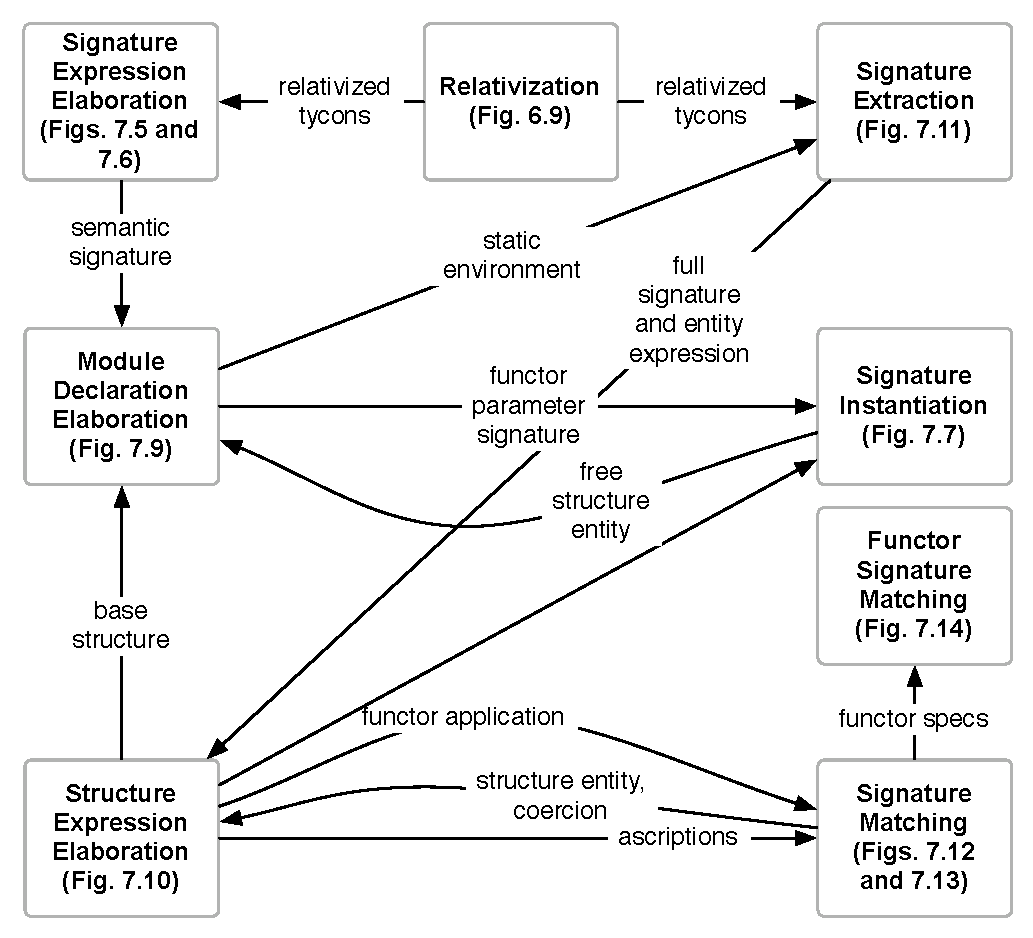
\includegraphics[scale=0.8]{figs/overview}
\end{center}
\caption{Map of elaboration processes}
\label{fig:overview}
\end{figure}
 
% \section{Why Higher-Order Functors?}
% The Fox project at CMU demonstrated that functors are valuable for the design and organization of extensible software systems. Shao~\cite{shao:parameterizedsigsandho}  demonstrates that higher-order functors are necessary for precisely expressing the import signature of a module that refers to externally defined functors. This idea is motivated by the \emph{fully functorized style} originally espoused by Tofte. 


\section{Elaboration Representations}
Elaboration is mainly concerned with the construction of a static environment. Secondarily, the elaborator produces typed abstract syntax, an entity environment, and an entity expression. The static environment contains the visible static information in the elaborated program. The static information comes in the form of semantic representations of signatures and type information. 

\begin{lstlisting}
sig
   type t [$\rho_t$] 
   type u = int 
   structure M [$\rho_M$] : sig type s [$\rho_s$] end
end
\end{lstlisting}
 
The entity environment contains static information that may have been occulted by shadowing and the functor actions describing the production of new static information during functor application. Much of elaboration is concerned with constructing the correct entity environment and using them to interpret entity paths. 

\section{Semantic Objects}
%!TEX root = ../main.tex
\begin{figure}
	\hrule
\[\begin{array}{rcll}
       s^p & ::= &  arity~|~\Sigma~|~\Sigma^f& \textrm{primary spec}\\
       \Sigma & ::= & \emptyset_{sig}~|~[x\mapsto (\rho,
       s^p)]\Sigma & \textrm{semantic signature}\\
       & ~~| & [x\mapsto \mathbb{C}^\lambda]\Sigma~|~[x\mapsto
       \mathbb{T}]\Sigma \\ 
	M & ::= & (\Sigma, R) & \textrm{full signature}\\
        \Sigma^f & ::= & \Pi\rho:\Sigma.\Sigma & \textrm{functor signature}\\
	F & ::= & (\Sigma^f, \psi) & \textrm{full functor signature}\\
        \gamma & ::= &
        \mathfrak{T}~|~\mathfrak{C}^\lambda~|~\Sigma~|~\Sigma^f & \textrm{static binding}\\
        & ~~| & (\rho, M)~|~(\rho,
        F) \\
	\Gamma & ::= & \emptyset_{se}~|~\Gamma[x\mapsto \gamma] &
        \textrm{static type environment}\\
\end{array}\]
The static bindings for structures and functors include the entity
variable to permit direct construction of entity paths during
signature extraction, structure path, and functor path elaboration.  
\hrule
\caption{Semantic representations}
\label{fig:semanticobjs}
\end{figure}
A semantic signature is a sequence of signature elements, symbol to spec bindings. Signature elements can be volatile ($s^p$), definitional ($\mathbb{C}^\lambda$), or a value spec ($\mathbb{T}$). Note that all signature spec elements must be relativized. Nonvolatile elements including definitional tycons $\mathbb{C}^\lambda$ and value specs $\mathbb{T}$ need only specify their fixed static description. Volatile primary specs ($s^p$) such open ones $arity$, structures $\Sigma$, and functors $\Sigma^f$ may be instantiated by signature matching and thus must have a corresponding binding in the entity environment indexed by entity variables. A \emph{full signature M} gives a full semantic description of a structure. It is comprised of a semantic signature $\Sigma$ and a structure entity $R$ that interprets all the open specifications in $\Sigma$. 

A semantic functor signature $\Sigma^f$ binds an entity variable for the functor parameter $\rho$ in the functor result signature. A full functor signature $F$ is comprised a semantic functor signature $\Sigma^f$ and a functor entity $\psi$ that when evaluated will interpret all the open specifications in the functor result signature. 

$\gamma$ is a static binding, to which the static environment $\Gamma$ maps identifiers. For value identifiers, the static description is a semantic type expression $\mathfrak{T}$. For tycon definitions, the static description is $\mathfrak{C}^\lambda$. There is no static binding for open tycon because all tycons are either defined or instantiated in the static environment.  For signature and functor signature identifiers, the static descriptions are semantic signatures ($\Sigma$) and semantic functor signature ($\Sigma^f$). For structure and functor identifiers, the static descriptions are full signatures and full functor signatures respectively. Some static binding (namely for structures and functors) consist of the full signature or full functor signature coupled with the entity variable for that structure or functor. The entity variable is used to construct entity paths during signature extraction and elaboration. 

Tycons in signatures and in static environments differ in that tycons
in the former will have been relativized during signature elaboration
or extraction. Unlike static environments that may be extended
throughout the elaboration process, signatures do not change. Hence to
ensure that volatile tycons in signatures have an appropriate
interpretation, they must be relativized with respect to the entity
environment. 

\begin{figure}
\begin{center}
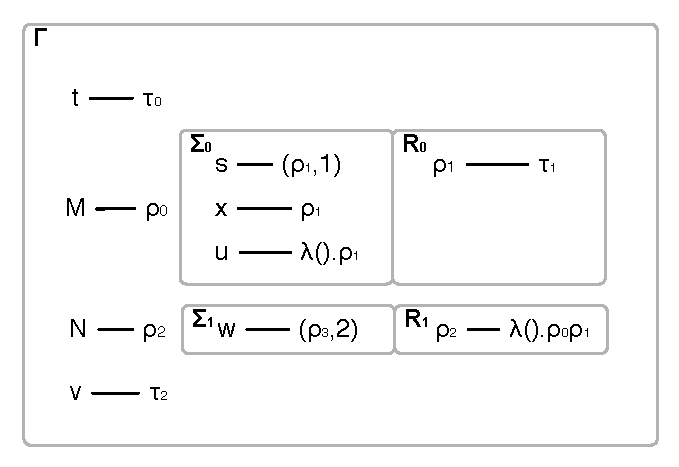
\includegraphics{figs/fig-staticenv-sigs}
\end{center}
\caption{Schematic of static environment}
\label{fig:staticenv-sigs}
\end{figure}

In Fig.~\ref{fig:staticenv-sigs}, the static environment depicted
exhibits the heterogeneous form of the definition. The first layer
contains semantic tycons, those types directly bound by the static
environment. The second layer consist of the tycons $s, u,$ and $w$ bound in semantic
signatures $\Sigma_0$ and $\Sigma_1$ embedded inside of the static
environment. These semantic signatures contain relativized tycons. The
full signature for structures also include the structure entity
expressions $R_0$ and $R_1$ which define the instantiation of the open
tycons in the corresponding semantic signature.  


\section{Notation}\label{sec:elabnotation}

If $p$ is a symbolic path and $\Sigma$ is a semantic signature, then $p\in\Sigma$ means that following $p$ in $\Sigma$ reaches a spec. If $p$ is a singleton, then $\Sigma$ must contain a binding $p\mapsto spec$. Otherwise, if $p$ is nonsingleton, then $p=xp'$ such that $x$ is a symbol and $p'$ is a symbolic path such that $\Sigma$ contains a binding $x\mapsto (\rho,\Sigma')$ and $p'\in\Sigma$. 

$\Sigma(p)$ is the spec reached by following $p$ in $\Sigma$. The notation $\EP(\Sigma,p)$ denotes the entity path associated with the signature spec referred to by symbolic path $p$. The entity path is comprised of the entity variables on the path to the element. For example, if the signature is $\Sigma = [A\mapsto(\rho_A,[B\mapsto (\rho_B, [t \mapsto (\rho_t, 0)])])]$, then $\Sigma_{ep}(A.B.t) = \rho_A\rho_B\rho_t$. The same notation is extended to static environments. 

Static environment lookup is expressed as $\Gamma(p)$ where $p$ is the symbolic path to the static binding. If $p$ is a singleton, then the static environment lookup would simply return the corresponding static binding. As will be demonstrated below, static environment lookup sometimes requires an entity environment lookup. This is the case when the component being looked up is a definitional tycon in a nonsingleton path. Depending on what kind of entity $p$ refers to, the lookup is handled differently:
\begin{description}
\item[tycon]
\begin{description}
\item[singleton path $p=x$] The semantic tycon is $\Gamma(x)$.
\item[nonsingleton $p=q.x$] $\Gamma(q)$ produces a full signature ($\Sigma_q,R_q$). Let $\Upsilon_q = \Upsilon^{clo}\Upsilon^{lcl}$ where $R_q = \langle \Upsilon^{lcl}, \Upsilon^{clo}\rangle$. 

If $\Sigma_q(x) = (\rho_x,n)$, then $\Gamma(p) = \Upsilon_q(\rho_x)$. 

If $\Sigma_q(x) = \mathbb{C}^\lambda$, then $\Gamma(p) = $ the interpretation of $\mathbb{C}^\lambda$ under $\Upsilon_q$. 

Note that all tycons are interpreted using the structure entity closest to the occurrence. 
\end{description}
\item[full signature or a full functor signature] $\Gamma(p)$ denotes a pair $(\vec{\rho}, M)$ such that $\vec{\rho}$ is the entity path to the structure static binding and $M$ is the full signature of that structure. For example, for $\Gamma=[A\mapsto(\rho_A,([B\mapsto(\rho_B, \Sigma_B)], R_A))]$, $\Gamma(A.B) = (\rho_A\rho_B, (\Sigma_B,R_A(\rho_A\rho_B)))$. 
\end{description}

\section{Elaboration Modes}
During elaboration, entity expressions are both produced and consumed to aid in typechecking. Elaboration occurs in two simultaneous modes: the \emph{direct mode} and the \emph{entity compilation mode}. Direct mode consists of core language type checking, direct construction of entity expressions (such as tycon declaration elaboration and signature instantiation), and evaluation of entity expressions from the static information uncovered during elaboration. The main results of this mode are a static environment mapping symbolic names to static descriptions and an entity environment mapping entity variables to entities. The evaluation of entity expressions may produce new entities which added to static and entity environments. The entity compilation mode compiles functor actions into entity expressions.   

Elaboration is entirely a compile-time process. The entity language is distinct from core and module languages. The language is parallel to the semantic representation and the syntactic language. Elaboration translates core and module languages to typed abstract syntax and entity expressions. The part of elaboration that produces entity expressions and declaration is called \emph{static entity compilation}. Because the entity language is intended to describe functor actions, which are not encoded in the typed abstract syntax, the two are complementary. When the elaborator reaches a functor application in the source, the corresponding application entity expression must be evaluated to produce the static information for the result. Entity expression evaluation yields structure entities. 
   
\section{Entity Compilation Mode}
Besides the direct elaboration mode for the evaluation of entity expressions, described in chapter~\ref{ch:entitycalc}, the elaborator must have an entity compilation mode that produces the entity expressions and semantic representations of the modules from the syntax. The process of the compilation mode is the bulk of the elaboration semantics. Entity expressions for both structures and functors are compiled from the raw implicitly typed abstract syntax trees and the contextual environments used during elaboration. The compilation mode elaboration is the subject of the remainder of this chapter. 

The compilation mode elaboration compiles abstract
syntax trees to entity expressions. All of elaboration takes place
under a static environment $\Gamma$. Recall that semantic
signatures pair all static primary components with entity variables
and replace all occurrences of such primaries with a canonical entity path to the corresponding static entity in the entity environment, which is calculated by relativization. Values are classified by their type. Structures are described by their full signature consisting of a structure entity and a signature. A functor static description is a full functor signature, comprised of a functor entity expression (\ie, a $\lambda$-expression) and a functor signature. The main elaboration judgments are the following:\\[-5mm]
 
\begin{tabular}{ll}
        $\Gamma,\Upsilon,\Sigma\vdash C^s \Rightarrow_{mt} \mathfrak{C}^s$ & monotype elaboration\\
        $\Gamma,\Upsilon,\Sigma\vdash C^\lambda \Rightarrow_{tyc} \mathfrak{C}^\lambda$ & tycon elaboration\\
        $\Gamma,\Upsilon,\Sigma\vdash T \Rightarrow_{te} \mathfrak{T}$ & type elaboration\\
\end{tabular}\\

The above judgments produce semantic monotypes/tycons/type expressions from syntactic ones. Tycon elaboration's sole role is during elaboration of tycon declarations (rule~\ref{eq:typedefdecl}). \\[-5mm]

\begin{tabular}{ll}       
        $\Upsilon\vdash \mathfrak{C}^s \searrow^{mt} \mathbb{C}^s$ & monotype relativization\\
        $\Upsilon,\Sigma\vdash \mathfrak{C}^\lambda \searrow^{tyc} \mathbb{C}^\lambda$ & tycon relativization\\
        $\Upsilon,\Sigma\vdash T \searrow^{te} \mathbb{T}$ & type expression relativization
\end{tabular}\\

The relativization judgment produce relativized tycons from syntactic ones. The entity environment $\Upsilon$ is used to relativize the nonlocally defined tycons. The signature $\Sigma$ is used to construct relativized entity paths for locally defined tycons. Signature extraction and elaboration rely on relativization. \\[-5mm]

\begin{tabular}{ll}      
        $\Gamma,\Upsilon,\Sigma\vdash sigexp \Rightarrow_{sig} \Sigma'$ & signature elaboration\\
        $\Gamma,\Upsilon,\Sigma\vdash fsgexp \Rightarrow_{fsg} \Sigma^f$ & functor signature elaboration\\
        $\Upsilon^{clo},\Upsilon^{lcl}\vdash \Sigma \uparrow \Upsilon^{lcl}$ & signature instantiation\\
        $\Gamma,\Upsilon\vdash d^m \Rightarrow_{decl} (\eta,\Gamma',\Upsilon')$ & module declaration elaboration\\
        $\Gamma,\Upsilon\vdash strexp \Rightarrow_{str} (M, \varphi)$ & structure expression elaboration\\
        $\Upsilon\vdash\Gamma\hookrightarrow \Sigma$ & signature extraction\\
        $\Upsilon\vdash(M,\varphi):\Sigma\Rightarrow_{match} (M_c,\varphi_c)$ & signature matching\\
        $\Upsilon\vdash F \preceq \Sigma^f \Rightarrow_{fsgmtch} (\psi_c, \theta_c)$ & functor signature matching
\end{tabular}

\section{Type Constructors}
The syntactic type language is a subset of the semantic tycon language. Before proceeding, the elaborator must first elaborate the syntactic types to semantic tycons. The elaboration is simply a syntax-directed recursive translation. 

The syntactic type language elaborates to the semantic type language. Elaboration interprets the symbolic paths in tycon application $p(\vv{C^s})$ and evaluates the application by standard $\beta$-reduction. Note that tycon elaboration $\Rightarrow_{tyc }$ elaborates and therefore reduces under $\lambda$-abstraction. This ensures that tycon definitions are fully reduced. Because $\lambda$s cannot be nested, this reduction is well-defined and normalizing. The normal form is defined as $\mathfrak{C}^{nf}$ in fig.~\ref{fig:semtypesystem}. 

\begin{figure}
\centering
\fixedCodeFrame{
\small
\setlength{\tabcolsep}{0ex}
\renewcommand{\arraystretch}{1.1}
~\\[2mm]
\fbox{$\Gamma,\Sigma\vdash C^s \Rightarrow_{mt} \mathfrak{C}^s$}

\begin{equation}
\Gamma,\Sigma\vdash \alpha \Rightarrow_{mt} \alpha
\label{eq:alpha}
\end{equation}

\begin{equation}
\infer{\Gamma,\Sigma\vdash p(\vv{C^s}) \Rightarrow_{mt}
 \mathfrak{C}^s_a}
{\begin{array}{c}
\Gamma,\Sigma\vdash C^s_i \Rightarrow_{mt} \mathfrak{C}^s_i~\forall i\in[1,|\vv{C^s}|]\\
(\mathsf{entpath}(\Gamma,\Sigma,p))(\vv{\mathfrak{C}^s}) \Downarrow_{tyc} \mathfrak{C}^s_a
\end{array}}
\label{eq:tycapp}
\end{equation}

\fbox{$\Gamma,\Sigma\vdash C^\lambda 
\Rightarrow_{tyc} \mathfrak{C}^\lambda$}

\begin{equation}
\infer{\Gamma,\Sigma\vdash \lambda\vec{\alpha}.C^s
  \Rightarrow_{tyc}\lambda\vec{\alpha}.\mathfrak{C}^s}
  {\Gamma,\Sigma\vdash C^s \Rightarrow_{mt} \mathfrak{C}^s}
% This rule is necessary to permit relativization of type definitions
% that area always enclosed by a single lambda. 
\end{equation}

\fbox{$\Gamma,\Sigma\vdash T \Rightarrow_{te} \mathfrak{T}$}

\begin{equation}
\infer{\Gamma, \Sigma\vdash \mathsf{typ}(C^s) 
\Rightarrow_{te} \mathsf{typ}(\mathfrak{C}^s)}
{\Gamma, \Sigma\vdash C^s \Rightarrow_{mt} \mathfrak{C}^s}
\end{equation}

\begin{equation}
\infer{\Gamma, \Sigma\vdash \forall\vec{\alpha}.C^s \Rightarrow_{te}
  \forall\vec{\alpha}.\mathfrak{C}^s}
{\Gamma, \Sigma\vdash C^s \Rightarrow_{mt} \mathfrak{C}^s}
\end{equation}

\begin{equation*}
\mathsf{entpath}(\Gamma,\Sigma,p) = \left\{ \begin{array}{ll}
\mathsf{EP}(\Sigma,p)& \textrm{if }p\in\Sigma\\
 \Gamma_{ep}(p) & \textrm{o.w.}
\end{array}
\right. 
\end{equation*}
}
\caption{Monotype and tycon elaboration}
\label{fig:tyconelab}
\end{figure} 

Note that the tycon may be occuring inside a signature spec, in which case it may refer to entity paths for preceding specs. 

\begin{lstlisting}
sig 
  type t
  type u = t
end
\end{lstlisting}

During the elaboration of the above, t will be given an entity variable. When elaborating the occurrence of tycon t in the definition of u, t is not the static environment. It can only be found in the partial semantic signature produced by elaborating the open spec for t. Signature specs may contain relativized tycons, entity paths,
referencing entities declared earlier in the same semantic signature. These preceding signature specs (forming a semantic signature $\Sigma$ itself)
help construct an entity path for symbolic paths not defined in the
static environment. Rule~\ref{eq:tycapp} uses $\entpath$ to calculate the entity path using static and entity environments. In order
to fully relativize such a symbolic path, the $\entpath$ metafunction
needs to first lookup the symbolic path in the preceding signature
specs $\Sigma$, which contains all the preceding specs in the current signature and only if that fails does it look up in the static environment.  


The type elaboration judgments preserve the well-kinding defined in chapter~\ref{ch:typesystem}.

\begin{lemma}[Monotype Elaboration Preserves Kinding]
If $\Gamma,\emptyset_{knds}\vdash C^s : \Omega$ and $\Gamma,\Upsilon\vdash C^s \Rightarrow_{mt} \mathfrak{C}^s$, then $\emptyset_{knds}\vdash \mathfrak{C}^s : \Omega$. 
\end{lemma}

\begin{lemma}[Tycon Elaboration Preserves Kinding]
If $\Gamma,\emptyset_{knds}\vdash C^\lambda : \Omega^n \Rightarrow
\Omega$ and $\Gamma,\Upsilon\vdash C^\lambda \Rightarrow_{tyc}
\mathfrak{C}^\lambda$, then $\emptyset_{knds}\vdash \mathfrak{C}^\lambda : \Omega^n \Rightarrow \Omega$.
\end{lemma}

\section{Signature Elaboration}
The role of signature elaboration is to relativize tycons, to reduce where type clauses to type definitions, and to decorate all specs corresponding to static entities with  entity variables. The elaboration judgment uses static and entity environment to interpret symbolic paths in tycon definitions. However, not all symbolic paths are bound in the static environment. For example, in the following signature, the type definition for u mentions tycon t which does not have a corresponding structure entity at this point, hence tycon t will not be in static and entity environment. 

\begin{lstlisting}
sig type t type u = t end
\end{lstlisting}

Rule~\ref{eq:specs} composes the result of elaborating the individual specs. Elaborating subsequent specs in the same signature will require a context (a signature) that includes all the previously elaborated specs $\Sigma$ and the newly elaborated spec $\Sigma'$.  

%!TEX root = ../principles.tex
\begin{figure}
\centering
\fixedCodeFrame{
\small
\setlength{\tabcolsep}{0ex}
\renewcommand{\arraystretch}{1.1}
~\\[2mm]
\fbox{$\Gamma,\Upsilon,\Sigma\vdash sigexp \Rightarrow_{sig} \Sigma'$}
	
\begin{equation}
\infer{\Gamma,\Upsilon,\Sigma\vdash x \Rightarrow_{sig} \Gamma(x)}
{\strut} 
\label{eq:emptysig}
\end{equation}

\begin{equation}
\infer{\Gamma,\Upsilon,\Sigma\vdash sigexp~\textbf{where type}~p = C^\lambda\Rightarrow_{sig}\mathsf{rebind}(p,\mathbb{C}^\lambda,\Sigma')}
	{\begin{array}{c}
	  \Gamma,\Upsilon,\Sigma\vdash sigexp\Rightarrow_{sig}\Sigma'\qquad
	  \Sigma'(p) = (\rho,n)\\ \Gamma,\Upsilon\vdash C^\lambda \Rightarrow_{tyc} \mathfrak{C}^\lambda\qquad 
          \Gamma,\Upsilon,\Sigma\Sigma'\vdash C^\lambda \searrow^{tyc} \mathfrak{C}^\lambda \\
          \Upsilon\vdash \mathfrak{C}^\lambda \searrow^{tyc} 
          \mathbb{C}^\lambda\qquad |\mathbb{C}^\lambda|=n
	 \end{array}} 
\label{eq:wheretype}
\end{equation}

\begin{equation}
\infer{\Gamma,\Upsilon,\Sigma\vdash \textbf{sig } specs \textbf{ end} \Rightarrow_{sig} \Sigma'}
	{\begin{array}{c}
	\Gamma,\Upsilon,\Sigma\vdash specs \Rightarrow_{specs} \Sigma'
	\end{array}} 
\label{eq:sigspecs}
\end{equation}

$\mathsf{rebind}(p,\mathbb{C}^\lambda,\Sigma)$ replaces the
binding $[x\mapsto (\rho,n)]$ in $\Sigma$ with $[x \mapsto 
\mathbb{C}^\lambda]$ where $p$ ends in $x$. 

\fbox{$\Gamma,\Upsilon,\Sigma\vdash specs \Rightarrow_{specs} \Sigma$}
\begin{equation}
\infer{\Gamma,\Upsilon,\Sigma\vdash \emptyset_{specs} \Rightarrow_{specs} \emptyset_{sig}}
{\strut}
\end{equation}

\begin{equation}
\infer{\Gamma,\Upsilon,\Sigma\vdash spec,specs \Rightarrow_{specs} \Sigma'\Sigma''}
{\Gamma,\Upsilon,\Sigma\vdash spec \Rightarrow_{spec} \Sigma' \qquad \Gamma,\Upsilon,\Sigma\Sigma'\vdash specs \Rightarrow_{specs} \Sigma''}
\label{eq:specs}
\end{equation}

}
\caption{Signature elaboration}
\label{fig:elabsig}
\end{figure}

\begin{figure}
	\centering
	\fixedCodeFrame{
	\small
	~\\[2mm]
	\fbox{$\Gamma, \Upsilon, \Sigma \vdash spec \Rightarrow_{spec} \Sigma'$}
\begin{equation}
\infer{\Gamma,\Upsilon,\Sigma\vdash\textbf{type
                  }\vec{\alpha}~t\Rightarrow_{spec} [t\mapsto (\rho,|\vec{\alpha}|)]}
{(\rho\textrm{ fresh in }\Gamma\textrm{ and
                  }\Upsilon)} 
\end{equation}
% Do we need to extend the static environment during elaboration of
% the subsequent specs? The only reason we might need to is to support
% relativization. I think we have to. 
\begin{equation}
\infer{\Gamma,\Upsilon,\Sigma\vdash\textbf{type }t=C^\lambda\Rightarrow_{spec} [t\mapsto \mathbb{C}^\lambda]}
{\Gamma,\Upsilon\vdash C^\lambda \Rightarrow_{tyc} \mathfrak{C}^\lambda\qquad \Upsilon,\Sigma\vdash \mathfrak{C}^\lambda \searrow^{tyc}
 \mathbb{C}^\lambda}
\label{eq:typedefspec}
\end{equation}

\begin{equation}
              \infer{\Gamma,\Upsilon,\Sigma\vdash\textbf{val }x:T
                 \Rightarrow_{spec} [x\mapsto\mathbb{T}]}
{\Gamma,\Upsilon\vdash T \Rightarrow_{te} \mathfrak{T}\qquad \Upsilon,\Sigma\vdash \mathfrak{T} \searrow^{tyc} \mathbb{T}}
\label{eq:valspec}
\end{equation}

\begin{equation}
\infer{\begin{array}{c}
    \Gamma,\Upsilon,\Sigma\vdash\textbf{structure }x :
                  sigexp
                  \Rightarrow_{spec} [x\mapsto
                  (\rho,\Sigma')]
\end{array}}
		{\begin{array}{c}
                    \Gamma,\Upsilon,\Sigma\vdash sigexp
                    \Rightarrow_{sig}
                    \Sigma'\qquad
                    (\rho~\textrm{fresh in }\Gamma\textrm{ and
                    }\Upsilon) 
              \end{array}}
\end{equation}

\begin{equation}
\infer{\begin{array}{c}
\Gamma,\Upsilon,\Sigma\vdash\textbf{functor }f(X: sigexp_1):sigexp_2\\
   \Rightarrow_{spec} [f\mapsto(\rho,\Pi\rho_x:\Sigma_1.\Sigma_2)]
\end{array}}
		{\begin{array}{c}
\Gamma,\Upsilon,\Sigma\vdash sigexp_1 \Rightarrow_{sig}
\Sigma_1 \qquad
(\rho_x\textrm{ and }\rho~\textrm{fresh in }\Gamma\textrm{ and }\Upsilon )\\
\Gamma,\Upsilon,\Sigma[X\mapsto(\rho_x,\Sigma_1)]\vdash
sigexp_2 \Rightarrow_{sig} \Sigma_2\\
% \qquad \psi=\langle\lambda\rho_x.\Sigma_2 ;
%  \Upsilon\rangle % [4/8/10] Is this the correct closure environment? Can \Sigma_2 mention local entities? Yes, but those are local, therefore, they should be interpreted locally and not by the closure, which only interpret nonlocal entities.  
\end{array}}
\label{eq:fctspec}
\end{equation}

	}
	\caption{Signature spec elaboration}
	\label{fig:elabspec}
\end{figure}   

Signature spec elaboration produces entity variables for each static
component (\emph{i.e.}, open type specs, structure spec, and functor
spec) and puts them in the resultant semantic
signature. Rules~\ref{eq:typedefspec} and~\ref{eq:valspec} relativize
semantic tycons and type expressions respectively. 

In particular, the signature $\Sigma$ is needed when relativizing specs in a signature $\Sigma'$ that contain symbolic paths defined within the same $\Sigma$. Latter specs can contain symbolic paths declared in earlier specs within the same signature. Because the signature is not yet fully elaborated and does not correspond to any full signature, it is neither defined in the static environment nor the entity environment, each of which only mapping paths defined outside of the signature currently being elaborated. 


Rule~\ref{eq:fctspec} elaborate the formal parameter signature $sigexp_1$ and then the functor body signature $sigexp_2$ with the signature context extended with a spec corresponding to the formal parameter. 

Let $AT(\cdot)$ denote the set of all atomic tycons ($\tau^n$) in $\cdot$. 
The following lemma guarantees that all tycons are fully relativized by the relativization judgment. 

\begin{lemma}
If $AT(\Sigma) = \emptyset$, for all $\Sigma_i\in\Gamma.AT(\Sigma_i)=\emptyset$, and $\Gamma,\Upsilon,\Sigma\vdash sigexp \Rightarrow_{sig} \Sigma'$, then $AT(\Sigma') = \emptyset$. 
\end{lemma}

\section{Signature Instantiation}\label{sec:siginst}

\begin{figure}
\centering
\fixedCodeFrame{
\small
\setlength{\tabcolsep}{0ex}
\renewcommand{\arraystretch}{1.1}
~\\[2mm]
\fbox{$\Upsilon^{clo}, \Upsilon^{lcl}_1\vdash \Sigma \uparrow \Upsilon^{lcl}_2$}
% Instantiation only returns the local entity environment for the
% realization 

\begin{equation}
\infer{\Upsilon^{clo},\Upsilon^{lcl}\vdash \emptyset_{sig} \uparrow \emptyset_{ee}}
{\strut} 
\label{eq:inst-empty}
\end{equation}

\begin{equation}
\infer{\Upsilon^{clo},\Upsilon^{lcl} \vdash [x \mapsto \mathbb{C}^\lambda]\Sigma \uparrow
  \Upsilon'}
{\Upsilon^{clo},\Upsilon^{lcl}\vdash \Sigma\uparrow\Upsilon'
 }
\end{equation}

\begin{equation}
\infer{\Upsilon^{clo},\Upsilon^{lcl}\vdash [x \mapsto \mathbb{T}]\Sigma \uparrow \Upsilon'}
{\Upsilon^{clo},\Upsilon^{lcl}\vdash \Sigma \uparrow \Upsilon'}
\end{equation}

\begin{equation}
\infer{\Upsilon^{clo},\Upsilon^{lcl} \vdash [x \mapsto (\rho, n)]\Sigma \uparrow
  [\rho \mapsto \tau^{n}]\Upsilon'}
{\Upsilon^{clo},\Upsilon^{lcl}[\rho\mapsto\tau^n]\vdash \Sigma \uparrow \Upsilon'\qquad(\tau\textrm{ is fresh
    in }\Upsilon^{clo}\textrm{ and }\Upsilon^{lcl})} 
\label{eq:inst-open}
 \end{equation}

\begin{equation}
\infer{\Upsilon^{clo},\Upsilon^{lcl}\vdash [x \mapsto (\rho,\Sigma')]\Sigma \uparrow
  [\rho\mapsto \langle \Upsilon', \Upsilon^{clo}\Upsilon^{lcl} \rangle]\Upsilon''}
{\Upsilon^{clo},\Upsilon^{lcl}\vdash \Sigma'\uparrow\Upsilon'\qquad
\Upsilon^{clo},\Upsilon^{lcl}[\rho\mapsto\langle\Upsilon',\Upsilon^{clo}\Upsilon^{lcl}\rangle]\vdash
\Sigma\uparrow\Upsilon''}
\label{eq:inst-str}
\end{equation}

% The closure entity environment here includes local entities. Will
% this give the incorrect realizations? 
\begin{equation}
\infer{\Upsilon^{clo},\Upsilon^{lcl}\vdash [x \mapsto (\rho, \Pi \rho_x:\Sigma_x.\Sigma_r)]\Sigma \uparrow
  [\rho\mapsto \langle \lambda \rho_x.\Sigma_r ; \Upsilon^{clo}\Upsilon^{lcl}\rangle]\Upsilon'}
{\Upsilon^{clo},\Upsilon^{lcl}[\rho\mapsto \langle \lambda \rho_x.\Sigma_r ; \Upsilon^{clo}\Upsilon^{lcl}\rangle]\vdash \Sigma\uparrow\Upsilon'}
\label{eq:inst-fct}
\end{equation}

}
\caption{Signature instantiation}
\label{fig:siginst}
\end{figure}


Signature instantiation produces a free instantiation of a given
semantic signature, where free is in the context of both a closure and
a local entity environment. Instantiation produces an entity
environment that is local, meaning exclusive of closure entity
environment bindings (see rule~\ref{eq:inst-empty}). 

Most of the
judgments ignore the signature element. The elements that matter are
the those corresponding to static entities. Rule~\ref{eq:inst-open}
produces a fresh atomic tycon $\tau^n$ of the appropriate arity
$n$. The tycon must be fresh in both closure and local entity
environments. Subsequent signature elements must be instantiated in
the context of the local entity environment extended with the binding
to the new tycon $[\rho\mapsto\tau^n]$. This new binding serves two
roles. First, it ensures that $\tau^n$ is not reused when
instantiating the rest of the signature elements. Second, the new
binding may be included as part of the closure entity environment when
instantiating a structure and functor specs.  

Rule~\ref{eq:inst-str} instantiates a structure spec by recursively
instantiating its semantic signature. The structure's semantic signature may mention
either entities in $\Upsilon^{clo}$ and $\Upsilon^{lcl}$, that is,
preceding entities in the same signature. The resulting entity environment
is combined with a closure $\Upsilon^{clo}\Upsilon^{lcl}$ to form a
structure entity. Rule~\ref{eq:inst-fct} instantiates a functor spec
by producing a functor entity contains a formal functor functor entity
expression $\lambda\rho_x.\Sigma_r$ and a closure entity
environment. 

\begin{lemma}[Signature Instantiation Terminates]
$\Upsilon\vdash \Sigma \uparrow \Upsilon'$ terminates.
\end{lemma}

\section{Top Level Declaration Elaborations}

\begin{figure}
\centering
\fixedCodeFrame{
\small
\setlength{\tabcolsep}{0ex}
\renewcommand{\arraystretch}{1.1}
~\\[2mm]

\fbox{$\Gamma,\Upsilon\vdash^{top} d^t~\mathsf{ok}$}

\begin{equation}
\infer{\Gamma,\Upsilon\vdash^{top} \circ~\mathsf{ok}}
{\strut}
\label{eq:topempty}
\end{equation}

\begin{equation}
\infer{\Gamma,\Upsilon\vdash^{top} \mathbf{signature}~x=sigexp,d^t~\mathsf{ok} }
{\Gamma,\Upsilon,\emptyset_{sig}\vdash sigexp \Rightarrow_{sig}
  \Sigma\qquad \Gamma[x\mapsto\Sigma],\Upsilon\vdash^{top} d^t~\mathsf{ok} }
\label{eq:sigdec}
\end{equation}

\begin{equation}
\infer{\Gamma,\Upsilon\vdash^{top} d^m, d^t~\mathsf{ok} }
{\Gamma,\Upsilon\vdash d^m \Rightarrow_{decl}
  (\eta,\Gamma',\Upsilon')\qquad \Gamma',\Upsilon'\vdash^{top} d^t~\mathsf{ok} }
\label{eq:topmoddec}
\end{equation}
}
\caption{Top level declarations}
\label{fig:toplevel}
\end{figure}


Elaboration of top level declaration is
straightforward. The semantics is given in Fig.~\ref{fig:toplevel}. Rule~\ref{eq:sigdec} elaborates a signature
expression and extends the static environment with a binding of the
signature name to the semantic signature. Rule~\ref{eq:topmoddec}
elaborates module declarations using the $\Gamma,\Upsilon\vdash d^m
\Rightarrow_{decl} (\eta,\Gamma',\Upsilon')$ judgment. The judgment
can safely discard the entity declarations from the module
declarations because top level declarations will not be wrapped in a
functor and therefore lead to functor actions. 

\section{Module Elaboration}\label{sec:modelab}

%!TEX root = ../principles.tex
\begin{figure}
\centering
\fixedCodeFrame{
\small
\setlength{\tabcolsep}{0ex}
\renewcommand{\arraystretch}{1.1}
~\\[2mm]
\fbox{$\Gamma,\Upsilon\vdash d^m \Rightarrow_{decl} (\eta, \Gamma', \Upsilon')$}

	\begin{equation} 
          \infer{\Gamma,\Upsilon\vdash \circ
            \Rightarrow_{decl} (\bullet, \emptyset_{se},
            \emptyset_{ee})}{\strut}  
          \label{eq:emptydecl}
        \end{equation}

        \begin{equation}
          \infer{\Gamma,\Upsilon\vdash \mathbf{val}~x=e,d^m
            \Rightarrow_{decl} (\eta, [x\mapsto\mathfrak{T}]\Gamma', \Upsilon')}
          {\Gamma \vdash e \Rightarrow_{core} \mathfrak{T} \qquad
            \Gamma[x\mapsto\mathfrak{T}], \Upsilon \vdash d^m \Rightarrow_{decl}
            (\eta, \Gamma', \Upsilon')}
          \label{eq:valdecl}
        \end{equation}

	\begin{equation} 
          \infer{\begin{array}{l} 
              \Gamma,\Upsilon\vdash \mathbf{type}~t=C^\lambda,d^m
              \Rightarrow_{decl}(\eta,[t\mapsto \mathfrak{C}^\lambda]\Gamma',\Upsilon')
	\end{array}}
	{\begin{array}{c}
            \Gamma,\Upsilon \vdash C^\lambda \Rightarrow_{tyc} \mathfrak{C}^\lambda\qquad
            \Gamma[t\mapsto \mathfrak{C}^\lambda],\Upsilon\vdash
            d^m\Rightarrow_{decl}(\eta,\Gamma',
            \Upsilon')
          \end{array}} 
        \label{eq:typedefdecl}
      \end{equation}

        \begin{equation} 
       \infer{\begin{array}{c}
           \Gamma,\Upsilon\vdash
         \mathbf{datatype}~\vec{\alpha}~t,d^m\\
         \Rightarrow_{decl}([\rho_t =_{tyc} \newx(n)]\eta, [t\mapsto
         \tau^n]\Gamma', [\rho_t\mapsto \tau^n]\Upsilon')
       \end{array}}
{\begin{array}{c}
    n=|\vec{\alpha}|\qquad
    \Gamma[t\mapsto\tau^n],\Upsilon[\rho_t\mapsto \tau^n]\vdash d^m \Rightarrow_{decl} (\eta, \Gamma',
    \Upsilon')\\ (\rho_t\textrm{ and }\tau\textrm{ are fresh})
\end{array}}
      \label{eq:dtdecl}
        \end{equation}

\begin{equation} 
          \infer{\begin{array}{c}
              \Gamma,\Upsilon\vdash \mathbf{structure}~X=strexp,d^m\\
  \Rightarrow_{decl} ([\rho=_{str}\varphi]\eta, [X\mapsto (\rho, M)]\Gamma',
  [\rho\mapsto R]\Upsilon')
\end{array}}
	{\begin{array}{c}
\Gamma,\Upsilon\vdash strexp\Rightarrow_{str} (M, \varphi)\qquad 
M = (\Sigma,R)\qquad (\rho~\textrm{fresh})\\
\Gamma[X\mapsto (\rho, M)],\Upsilon[\rho\mapsto R]\vdash d^m\Rightarrow_{decl}(\eta, \Gamma', \Upsilon')
	\end{array}} 
      \label{eq:strdecl}
\end{equation}


	\begin{equation} 
          \infer{\begin{array}{c}
              \Gamma,\Upsilon\vdash
              \mathbf{functor}~f(X:sigexp)=strexp,d^m \\
              \Rightarrow_{decl} ([\rho=_{fct}\theta]\eta, [f\mapsto(\rho,(\Pi\rho_x:\Sigma_x.\Sigma_{res},\psi))]\Gamma',
              [\rho\mapsto\psi]\Upsilon')
            \end{array}}
	        {\begin{array}{c} 
                    \Gamma,\Upsilon, \emptyset_{sig} \vdash
                    sigexp\Rightarrow_{sig} \Sigma_x\qquad
                    \Upsilon,\emptyset_{ee}\vdash \Sigma_x \uparrow
                    \Upsilon_x \\
                    R_x = \langle \Upsilon_x,\Upsilon \rangle\\
                    \Gamma[X\mapsto(\rho_x, (\Sigma_x,
                   R_x))],\Upsilon[\rho_x\mapsto R_x]\vdash
                    strexp\Rightarrow_{str}((\Sigma_{res},\_),\varphi)\\
                    % \Upsilon_\Delta is out of scope at the
                    % declaration level, so it is dropped. 
        \theta =
        \lambda\rho_x.\varphi\qquad \psi =
        \langle\theta;\Upsilon\rangle\\
	\Gamma [f\mapsto(\rho,(\Pi
        \rho_x:\Sigma_x.\Sigma_{res},\psi))],
        \Upsilon[\rho\mapsto\psi]\vdash
        d^m \Rightarrow_{decl}(\eta,\Gamma',\Upsilon')\\
        % No need for extending entity environment because \rho_F
        % won't be looked up
	(\rho_x,\rho~\textrm{fresh})\\
        %\Gamma, \Upsilon \vdash \emptyset_{se}\gamma \hookrightarrow (M_{ext}, \eta_{ext})
	         \end{array}} 
               \label{eq:fctdecl}
        \end{equation}
}
\vspace{1em}
The resultant $\Upsilon$ must be the local entity environment in order
for the structure expression judgment for struct $d^m$ end to properly
construct a structure realization. 
\caption{Module declaration elaboration}
\label{fig:elabmod}
\end{figure}

\begin{figure}
\centering
\fixedCodeFrame{
\small
~\\[2mm]
\fbox{$\Gamma,\Upsilon\vdash strexp \Rightarrow_{str} (M,\varphi)$}
	\begin{equation} 
\infer{\Gamma,\Upsilon\vdash p \Rightarrow_{str} (M, \vec{\rho})}
	          {\Gamma(p)=(\vec{\rho}, M)} 
\label{eq:strpath}
\end{equation}

	\begin{equation} 
\infer{\Gamma,\Upsilon\vdash \mathbf{struct}~d^m~\mathbf{end}
  \Rightarrow_{str} ( (\Sigma,\langle \Uloc,\Upsilon\rangle),\llparenthesis\eta\rrparenthesis)}
	{\begin{array}{c}
\Gamma,\Upsilon\vdash d^m\Rightarrow_{decl}(\eta,\Gamma', \Uloc)\qquad
\Upsilon \Uloc \vdash\Gamma'\hookrightarrow \Sigma
\end{array}} 
\label{eq:basestr}
\end{equation}

% [4/8/2010] How do local environments work with functor entities? 
\begin{equation} 
\infer{\begin{array}{c}
\Gamma,\Upsilon\vdash p(strexp)\Rightarrow_{str}
((\Sigma_{body},R_{app}),\varphi_{app})
\end{array}}
	{\begin{array}{c}
\Gamma(p) = (\vec{\rho}, (\Pi X:\Sigma_{par}.\Sigma_{body}, \langle\theta; \Upsilon'\rangle))\\
\Gamma,\Upsilon\vdash strexp\Rightarrow_{str}
(M,\varphi)\\ 
\Upsilon\vdash (M,\varphi) : \Sigma_{par} \Rightarrow_{match} (R_{c},\varphi_{c})\\
\varphi_{app} = \vec{\rho}(\varphi_{c})\qquad \Upsilon\vdash \varphi_{app} \Downarrow_{str} R_{app}
\end{array}}
\label{eq:strapp}
\end{equation}

	\begin{equation} 
\infer
	{\Gamma,\Upsilon\vdash \mathbf{let}~d^m~\mathbf{in}~strexp\Rightarrow_{str}(M,\mathbf{let}~\eta_{def}~\mathbf{in}~\varphi)}
	{\begin{array}{c}\Gamma,\Upsilon\vdash d^m\Rightarrow_{decl}(\eta_{def},\Gamma_{def},\Upsilon_{def})\\ \Gamma_{def},\Upsilon_{def}\vdash strexp\Rightarrow_{str}(M, \varphi)
\end{array}} 
\label{eq:letexp}
\end{equation}

\begin{equation} 
\infer{\begin{array}{c}
\Gamma,\Upsilon\vdash strexp : sigexp
 \Rightarrow_{str} ((\Sigma_{spec},R_c),\varphi_c)
\end{array}}
{\begin{array}{c}
	   \Gamma,\Upsilon,\emptyset_{sig}\vdash sigexp \Rightarrow_{sig} \Sigma_{spec} \qquad
	   \Gamma,\Upsilon\vdash strexp \Rightarrow_{str} (M_{u},\varphi_{u})\\
	   \Upsilon\vdash (M_{u},\varphi_u) : \Sigma_{spec} \Rightarrow_{match} (R_c,\varphi_{c})
\end{array}} 
\label{eq:transascription}
\end{equation}
     
 \begin{equation} 
\infer{\begin{array}{c}
\Gamma,\Upsilon \vdash strexp :> sigexp 
\Rightarrow_{str}
   ((\Sigma_{spec},\langle\Upsilon_{spec},\Upsilon\rangle),
   \varphi_{c})
\end{array}}
{\begin{array}{cc}
\Gamma,\Upsilon,\emptyset_{sig}\vdash sigexp
     \Rightarrow_{sig} \Sigma_{spec}\qquad
   \Gamma,\Upsilon\vdash strexp \Rightarrow_{str} (M_u, \varphi_u)\\
  \Upsilon\vdash (M_u,\varphi_u) : \Sigma_{spec}
  \Rightarrow_{match} (R_{c},\varphi_{c})\\
  \Upsilon, \emptyset_{ee} \vdash \Sigma_{spec} \uparrow \Upsilon_{spec}
% Does it matter whether we return the uncoerced or coerced varphi?
% The compiler returns the coerced version.  
\end{array}
}
\label{eq:opaqueascription}
\end{equation}

}
\caption{Structure expression elaboration}
\label{fig:strexpelab}
\end{figure}



The module elaboration judgment calls for a static environment and an entity environment as its context. The static environment serves to elaborate tycons and structures, by looking up symbolic paths. The entity environment plays a role in signature elaboration and instantiation of functor parameters. 

Fig.~\ref{fig:elabmod} gives the rules for elaborating module declarations. The judgment computes an entity declaration, a static environment, and an entity environment for the module declarations. The two environments will only contain bindings representing the information in the module declarations and not the closure. Each module declaration elaboration rule calculates a semantic representation of the declaration value (\emph{i.e.}, type expressions, (definitional) tycons, atomic tycons, full signatures, and full functor signatures) and binds that representation in the static environment (and the entity environment if the entity in question is primary). 

Rules~\ref{eq:valdecl} and~\ref{eq:typedefdecl} elaborate values to a
semantic type expression and syntactic tycon to semantic tycon
respectively. Rule~\ref{eq:valdecl} assumes a core expression elaboration (typechecking) judgment of the form $\Gamma\vdash e \Rightarrow_{core} \mathfrak{T}$, which is standard. Neither of these produce any entity declarations and
entity environment because they do not contain static
entities. Rule~\ref{eq:dtdecl} generates a fresh atomic tycon $\tau^n$
for a datatype. This atomic tycon is bound in both the static and
entity environments. The elaborator further produces an entity
declaration $\rho_t =_{tyc} \newx(n)$ that records the functor action
attributed to the datatype declaration. The entity declaration is
reserved for evaluation upon functor application of the possible
enclosing functor. When evaluated, it will produce another atomic
tycon distinct from the $\tau^n$ generated here. Rule~\ref{eq:strdecl}
elaborates the structure expression to a full signature and a
structure entity expression. Rule~\ref{eq:fctdecl} elaborates a
functor declaration via several steps: 
\begin{enumerate}
\item elaborate the functor parameter signature $\Sigma_x$
\item instantiate it $\Upsilon_x$
\item form a full signature using the result of the previous two steps $(\Sigma_x,R_x)$ where $R_x=\langle \Upsilon_x,\Upsilon\rangle$. 
\item elaborate the functor body using a static environment extended with this full signature and the entity environment extended with the structure entity 
\item form a full functor signature, a functor entity, and a functor entity expression using the structure entity expression from above
\end{enumerate}

Fig.~\ref{fig:strexpelab} elaborates a structure expression into a full signature and structure entity expression. Rule~\ref{eq:strpath} elaborates a structure path. The structure entity expression is an entity path, calculated by accumulating the entity variables in $\Gamma$ leading up to the element denoted by $p$. Rule~\ref{eq:basestr} must extract a semantic signature from the static environment produced by elaborating the base structure declarations. Rule~\ref{eq:strapp} elaborates a functor application in several steps:
\begin{enumerate}
\item looks up the entity path and full functor signature of the functor denoted by symbolic path $p$
\item elaborates the argument structure
\item coerces the argument structure and structure entity expression using the functor parameter signature by signature matching
\item forms the structure entity expression for the application 
\item evaluates the structure entity expression using the current entity environment
\end{enumerate}

Rule~\ref{eq:letexp} elaborates structure let expressions in the expected way. Rule~\ref{eq:transascription} elaborates transparent ascription by signature matching. Rule~\ref{eq:opaqueascription} elaborates opaque ascription by signature matching and then instantiating the spec signature to get fresh types for the open type specs. 

% Is the opaque ascription rule totally correct? It seems that using the spec signature and free instantion might be too much. 

An important invariant that must be maintained for module declaration elaboration is that all the atomic tycons in the static environment are also in the entity environment. This property guarantees that all atomic tycons can be relativized by the entity environment. 

\begin{lemma}
If $AT(\Gamma) \subseteq AT(\Upsilon)$ and $\Gamma,\Upsilon\vdash d^m \Rightarrow_{decl} (\eta,\Gamma',\Upsilon')$, then $AT(\Gamma') \subseteq AT(\Upsilon')$. 
\end{lemma}

The relationship between the semantic signature $\Sigma$ and structure
entity $R$ produced by elaboration is precisely related. $R$ is said
to \emph{interpret} $\Sigma$, which is defined as follows: 

\begin{definition}
$\Upsilon$ interprets $\Sigma$ if for all specs in $\Sigma$, one of the
following must be true:
\begin{enumerate}
\item If the spec is open$(\rho,n)$, then $\Upsilon(\rho)=\tau^n$
  or $\Upsilon(\rho)=\mathbb{C}^\lambda$ such that $\Upsilon\vdash
  \mathbb{C}^\lambda :: \Omega^n \to \Omega$. 
\item If the spec is a structure $(\rho,\Sigma')$, then $\Upsilon(\rho)=R'$ and $R'$ interprets $\Sigma'$. 
\item If the spec is a functor $(\rho,\Sigma^f)$, then 
  $\Upsilon(\rho)=\psi$. 
\end{enumerate}
\end{definition}

\begin{lemma}
If $\Upsilon$ interprets the extracted signature of $\Gamma$ and 
$\Gamma,\Upsilon\vdash strexp \Rightarrow_{str} ((\Sigma, R),
\varphi)$, then $R$ interprets $\Sigma$.
\end{lemma}

\section{Signature Extraction}\label{sec:sigextract}

%!TEX root = ../principles.tex

% Observation: Don't need the entire static environment as context
% because all symbolic names should have already been reduced
% away. The place where the entire static environment does play a role
% is in relativization of type expressions for values and (derived) tycon
% expressions. 

% There are some fundamental flaws in the rules as given. First, there
% is no base case, for the empty static environment. That would
% establish what the realization part of the resultant full signature
% really is. Second, none of the rules extend the realization part of
% the full signature at this point. Thus, I expect the resultant
% realization to end up empty anyway. 

\begin{figure}
	\centering
	\fixedCodeFrame{
	\small
        ~\\[2mm]
	\fbox{$\Upsilon\vdash \Gamma \hookrightarrow \Sigma $}
               \begin{equation}
                 \infer{\Upsilon\vdash\emptyset_{se}\hookrightarrow
                   \emptyset_{sig}}
                 {\strut}
               \end{equation}

		\begin{equation} 
                  \infer{\Upsilon\vdash
                    [x\mapsto \mathfrak{T}]\Gamma \hookrightarrow
                  [x\mapsto \mathbb{T}]\Sigma_r
                  }
		{\begin{array}{c}
                  \Upsilon\vdash \mathfrak{T} \searrow^{te}
                  \mathbb{T}\qquad
                  \Upsilon\vdash \Gamma \hookrightarrow \Sigma_r
                \end{array}} 
\label{eq:extraval}
            \end{equation}
% The value binding rule doesn't add any entity decl. It merely adds a value spec with a relativized version of value binding's type.

% There are no open tycon bindings in the static environment. All tycons in the static environment are defined or instantiated. 
% Perhaps combine \upharpoonright and C_{ep}() notation together because one is just an extension to type expressions
              %\begin{equation} \infer{\begin{array}{c} C_{ep},C_{elab}\vdash
               % [q\mapsto[=t]]\Gamma\\ \hookrightarrow
                %(([q\mapsto (\rho, \mathsf{arity}(t))]\Sigma, \Upsilon),
                %\eta)\end{array}}
              %{C_{ep},C_{elab}\vdash\Gamma\hookrightarrow((\Sigma,\Upsilon),
               % \eta)\qquad C_{ep}(t)=[\rho]} & \\[5mm]
              \begin{equation} 
\infer{\Upsilon\vdash [t\mapsto \mathfrak{C}^\lambda]\Gamma \hookrightarrow [t\mapsto \mathbb{C}^\lambda]\Sigma_r}
{\Upsilon\vdash \mathfrak{C}^\lambda
  \searrow^{tyc} \mathbb{C}^\lambda\qquad \Upsilon\vdash \Gamma \hookrightarrow
  \Sigma_r}
\label{eq:extratypedef}
\end{equation}

% SML/NJ's representation of tycon entities included type definitions
% (represented by an entity path). In this new semantics, there is no
% need for any form other than new(arity). 
% The question remains, what is the relationship between the scoping
% in the entity environment and in the static environment. That is to
% say, do we expect \Upsilon^{-1}(\tau^n) to be anything other than
% singleton? If so, what is an example?
\begin{equation} 
\infer{\Upsilon\vdash[t\mapsto\tau^n]\Gamma \hookrightarrow [t\mapsto (\rho, n)]\Sigma_r}
{\inv(\Upsilon,\tau^n)=\rho\qquad\Upsilon\vdash
  \Gamma \hookrightarrow\Sigma_r} 
\label{eq:extraatomictyc}
\end{equation}

% The interesting part about producing a tycon spec is how we compute the entity variable. The tycon definition may be local, in which case we can reuse that tycon's (RHS) entity variable. Otherwise, we need to produce a new entity variable and a corresponding entity declaration mapping this new entity variable to a CONSTtyc or a VARtyc for new and nonlocal tycons respectively. 
% What we need is a judgment that produces an entity variable, entity environment, and entity declarations from a static entity.
\begin{equation}
  \infer{\begin{array}{c}
      \Upsilon\vdash[x\mapsto (\rho, (\Sigma_1,R_1))]\Gamma_r\hookrightarrow [x\mapsto
                (\rho,\Sigma_1)]\Sigma_r
              \end{array}}
              {\begin{array}{c}
                  \Upsilon\vdash\Gamma_r\hookrightarrow \Sigma_r
                \end{array}}
\label{eq:extrastr}
            \end{equation}

% The structure binding rule first looks up the entity path for the full signature 
% If the structure has an entity path which is a singleton, then it uses that as entity variable in the structure spec we are producing. 
% If the entity path is not singleton, then the entdec is a structure e_new = ep such that ep is the non-singleton entity path. It is this e_new that is used in the structure spec. 
% Otherwise, no entity path exists yet so we produce a CONSTstr with the realization from the full signature, mapping a e_new to it. 
% In the latter two cases, the entity is not local so we need to add a
% local version of the entity to the entity environment, mapping e_new
% to rlzn.  
              \begin{equation} 
                \infer{\Upsilon\vdash[f\mapsto (\rho, (\Sigma^f_1,\psi))]\Gamma_r \hookrightarrow [f\mapsto (\rho,\Sigma^f_1)]\Sigma_r}
              {\begin{array}{c}
                 \Upsilon\vdash\Gamma_r\hookrightarrow\Sigma_r
              \end{array}} 
\label{eq:extrafct}
              \end{equation}

              % Ignoring signature and functor signature
              % bindings. Since this is the cumulative static
              % environment, it may contain top-level declared
              % signatures and functor signatures. 
             %\begin{equation}
             %\infer{\Upsilon\vdash[x\mapsto \Sigma]\Gamma\hookrightarrow \Sigma'}
             %{\Upsilon\vdash\Gamma\hookrightarrow \Sigma'}
             %\end{equation}

             %\begin{equation}
             %\infer{\Gamma_0,\Upsilon\vdash[x\mapsto\Sigma^f]\Gamma\hookrightarrow (M,\eta)}
             %{\Gamma_0,\Upsilon\vdash\Gamma\hookrightarrow (M,\eta)} 
             %\end{equation}

	}
\caption{Signature extraction}
\label{fig:extractsig}
\end{figure}

Fig.~\ref{fig:extractsig} gives the rules for signature extraction, the process of synthesizing a semantic signature for a structure given only the static environment produced by elaborating that structure and an entity environment. Because the signature must contain only relativized type expressions and tycons, rules~\ref{eq:extraval} and~\ref{eq:extratypedef} must relativize the semantic type expression and tycon in the static environment. Rule~\ref{eq:extraatomictyc} produces a spec from an atomic tycon binding, which specifies the arity $n$ of the tycon. The rule looks up the atomic tycon in the ``inverse'' of $\Upsilon$. This rule assumes that $\Upsilon$ and $\Gamma$ are synchronized. In particular, since $t$ is a local name in the static environment (\emph{i.e.}, its binding is not nested inside some signature in $\Gamma$), $\tau^n$ should also be local in $\Upsilon$ and therefore have a singleton entity path. 
 
\begin{lemma}[Synchronization of Static and Entity Environments]
If $\Gamma,\Upsilon \vdash d^m \Rightarrow_{decl} (\eta, \Gamma', \Upsilon')$ and $EV(\Gamma)\subseteq dom(\Upsilon)$, then $EV(\Gamma')\subseteq dom(\Upsilon')$. 
\end{lemma}

For full signatures and full functor signatures, signature extraction is simple. Rules~\ref{eq:extrastr} and~\ref{eq:extrafct} forms structure and functor specs by projecting out the entity variable and semantic signature (or semantic functor signature) from the static environment mapping for the structure and functor respectively. 

\section{Signature Matching}\label{sec:sigmatch}

\begin{figure}
\centering
\fixedCodeFrame{
\small
\setlength{\tabcolsep}{0ex}
\renewcommand{\arraystretch}{1.1}

~\\[2mm]

\fbox{$\Upsilon\vdash (M, \varphi) : \Sigma \Rightarrow_{match} (R_c,\varphi_{c})$}

\begin{equation}
\infer{\Upsilon\vdash
  ((\Sigma_{a},\langle\Upsilon_{a},\Upsilon^{clo}\rangle), \varphi) : \Sigma_{s}
  \Rightarrow_{match} (
  \langle\Upsilon',\Upsilon\rangle,\letx~\rho_u=\varphi~\inx~\llparenthesis \eta \rrparenthesis)}
{\begin{array}{c}
    (\rho_u\textrm{ is fresh in }\Upsilon)\qquad
    \Upsilon_{a}\Upsilon^{clo}\Upsilon, \Sigma_{a},\rho_u \vdash \Sigma_{s}
    \Rightarrow_{coerce} (\Upsilon', \eta)
 \end{array}}
\label{eq:sigmatch}
\end{equation}
}
\caption{Signature matching elaboration}
\label{fig:sigmatch}
\end{figure}
\begin{figure}
\centering
\fixedCodeFrame{
\small
\setlength{\tabcolsep}{0ex}
\renewcommand{\arraystretch}{1.1}
~\\[2mm]
\fbox{$\Upsilon,\Sigma_a,\rho_u\vdash \Sigma_s \Rightarrow_{coerce}
  (\Upsilon', \eta)$}

\begin{equation}
\infer{\Upsilon,\Sigma_a, \rho_a \vdash
  \emptyset_{sig} \Rightarrow_{coerce} (\emptyset_{ee}, \bullet)}
{\strut}
\label{eq:coerceempty}
\end{equation}

\begin{equation}
\infer{\Upsilon,\Sigma_a, \rho_a \vdash [x\mapsto
  \mathbb{T}]\Sigma_s \Rightarrow_{coerce} (\Upsilon', \eta)}
{\begin{array}{c}
\Upsilon \vdash \Sigma_a(x) \equiv \mathbb{T}\\
\Upsilon ,\Sigma_a, \rho_a \vdash \Sigma_s  \Rightarrow_{coerce}
(\Upsilon', \eta)
\end{array}}
\label{eq:coerceval}
\end{equation}


\begin{equation}
\infer{\begin{array}{c}
\Upsilon,\Sigma_a,\rho_u\vdash 
  [t\mapsto(\rho, n)]\Sigma_s\\
 \Rightarrow_{coerce}
 ([\rho\mapsto\Upsilon(\rho_a)]\Upsilon',[\rho=_{def}\rho_u\rho_a]\eta)
\end{array}}
{\begin{array}{c}
\Sigma_a(t) = (\rho_a, n')\qquad
\Upsilon, \Sigma_a, \rho_a \vdash \Sigma_s
  \Rightarrow_{coerce} (\Upsilon',\eta)\qquad n = n'
  \end{array}
}
\label{eq:coerceopen}
\end{equation}

\begin{equation}
\infer{\Upsilon,\Sigma_a,\rho_u\vdash
  [t\mapsto(\rho,n)]\Sigma_s 
  \Rightarrow_{coerce} ( 
  [\rho\mapsto\mathfrak{C}^\lambda]\Upsilon', [\rho=_{def}\mathbb{C}^\lambda]\eta)}
{\begin{array}{c}
\Sigma_a(t) = \mathbb{C}^\lambda\qquad |\mathbb{C}^\lambda| = n\qquad \Upsilon\vdash \mathbb{C}^\lambda = \mathfrak{C}^\lambda\\
\Upsilon, \Sigma_a, \rho_u \vdash \Sigma_s \Rightarrow_{coerce} (\Upsilon', \eta)
\end{array}}
\label{eq:coerceopenwithdef}
\end{equation}

\begin{equation}
\infer{\Upsilon,\Sigma_a,\rho_u \vdash [t\mapsto\mathbb{C}^{\lambda}_s]
  \Sigma_s \Rightarrow_{coerce} (\Upsilon',\eta)}
{\begin{array}{c}
\Sigma_a(t) = 
\mathbb{C}^{\lambda}_a\qquad
\Upsilon \vdash \mathbb{C}^{\lambda}_a \equiv \mathbb{C}^{\lambda}_s \\
\Upsilon,\Sigma_a,\rho_u \vdash \Sigma_s
\Rightarrow_{coerce} (\Upsilon',\eta)
\end{array}}
\label{eq:coercedefdef}
\end{equation}

\begin{equation}
\infer{\Upsilon,\Sigma_a,\rho_u \vdash [t\mapsto\mathbb{C}^{\lambda}_s]
  \Sigma_s \Rightarrow_{coerce} (\Upsilon',\eta)}
{\begin{array}{c}
\Sigma_a(t) = (\rho,n)\qquad
n=|\mathbb{C}^{\lambda}_s|\qquad\Upsilon\vdash\mathbb{C}^\lambda_s\equiv\Upsilon(\rho) \\
\Upsilon,\Sigma_a,\rho_u \vdash \Sigma_s
\Rightarrow_{coerce} (\Upsilon',\eta)
\end{array}}
\label{eq:coercedefwithdt}
\end{equation}

\begin{equation}
\infer{\Upsilon,\Sigma_a,\rho_u \vdash
  [x\mapsto (\rho_s,\Sigma_s)]\Sigma_s \Rightarrow_{coerce}
  (\Upsilon',[\rho_s = \varphi_c]\eta' )}
{\begin{array}{c}
\Sigma_a(x) = (\rho_x,\Sigma_x)\\
\Upsilon\vdash ((\Sigma_x, \Upsilon(\rho_x)), \rho_u\rho_x) : 
\Sigma_s \Rightarrow_{match} ((\Sigma_{c},R_{c}), \varphi_c)\\
\Upsilon[\rho_s\mapsto R_c],\Sigma_a,\rho_u\vdash \Sigma_s \Rightarrow_{coerce}
(\Upsilon',\eta')
\end{array}}
\label{eq:coercestr}
\end{equation}

\begin{equation}
\infer{\Upsilon,\Sigma_a,\rho_u \vdash
  [f\mapsto(\rho_s,\Sigma^f_s)]\Sigma_s \Rightarrow_{coerce}
  ([\rho_s \mapsto \psi_c]\Upsilon',[\rho_s = \theta_c]\eta)}
{\begin{array}{c}
\Sigma_a(f) = (\rho_a,\Sigma^f_a)\\ \Upsilon \vdash
((\Sigma^f_a, \Upsilon(\rho_a)),  \rho_u\rho_a ) : \Sigma^f_s
\Rightarrow_{fsgmtch} (\psi_c, \theta_c)\\
\Upsilon[\rho_s\mapsto \psi_c],\Sigma_a,\rho_u\vdash \Sigma_s
\Rightarrow_{coerce} (\Upsilon',\eta)\\
\end{array}
}
\label{eq:coercefct}
\end{equation}
}
\caption{Structure signature matching}
\label{fig:specmtch}
\end{figure}


Signature matching plays three principal roles during elaboration. It
coerces functor arguments to the form dictated by the functor
parameter signature in
rule~\ref{eq:strapp}. Rules~\ref{eq:transascription}
and~\ref{eq:opaqueascription} use signature matching to constrain the
full signature of the structure for transparent and opaque ascription
respectively. Figs.~\ref{fig:sigmatch} and~\ref{fig:specmtch} describe 
the signature matching judgment and its subsidiary judgment respectively. The main judgment for signature matching $\Upsilon\vdash(M,\varphi):\Sigma\Rightarrow_{match} (R_c,\varphi_c)$ forms the \emph{coercion structure entity expression} $\varphi_c$ which binds the uncoerced, original entity expression to a fresh entity variable $\rho_u$ for use by the coercion entity declarations $\eta$. In general, $\eta$ may alias components of $\varphi$ as is in the case in rule~\ref{eq:coerceopen}.  The coercion structure entity expression needs both $\varphi$ and $\eta$ because the elaborator needs to evaluate $\varphi$ at least for its functor actions and $\eta$ are the actual exported entity variables. The entity environment for signature matching is a composite of the context $\Upsilon$, actual structure local environment $\Upsilon_a$, and actual structure closure environment $\Upsilon^{clo}$. All three are necessary because $\Upsilon$ closes the spec signature $\Sigma_s$, $\Upsilon_a$ the actual $\Sigma_a$, and $\Upsilon^{clo}$ the local environment $\Upsilon_a$. 

A subsidiary judgment $\Upsilon,\Sigma_a,\rho_u\vdash \Sigma_s \Rightarrow_{coerce} (\Upsilon', \eta)$ matches actual structure components to individual specs. The actual structure signature $\Sigma_a$ is used to match against each spec. The entity variable $\rho_u$ provides access to the uncoerced structure entity expression in case the elaborator needs to alias components. The judgment will produce both a semantic signature and a local entity environment, used by the match judgment to produce a coerced full signature. 

Rule~\ref{eq:coerceempty} matches against an empty spec signature, in
which case the coercion signature, entity environment, and entity
declarations are empty. Rule~\ref{eq:coerceval} matches value specs
only when the value's type expressions are equivalent when interpreted
under the entity environment. For open tycon specs, there are two
cases. Rule~\ref{eq:coerceopen} matches an open tycon spec against an
open tycon spec in actual. In that case, the rule will use the
structure entity for the actual and an alias to the entity path for
the actual $\rho_u\rho_a$ for the entity
declaration. Rule~\ref{eq:coerceopenwithdef} matches an open tycon
spec against a definitional tycon spec in the actual. The arities of
the definitional tycon and the open tycon spec must match
up. Rule~\ref{eq:coercedefdef} matches a definitional tycon spec in
the spec signature to a definitional tycon spec in the actual. Again,
this match requires the equivalence of the spec and actual
definitional tycons interpreted under the entity
environment. Rule~\ref{eq:coercedefwithdt} matches a definition tycon
spec in the spec signature to an open tycon in the actual, which should be consistent with the tycon in entity environment $\Upsilon(\rho)$. Rules~\ref{eq:coercestr} and \ref{eq:coercefct} match structure and functor specs respectively. Being specs for entities, these rules must produce a new entity environment binding and entity declaration. Rule~\ref{eq:coercestr} forms the bindings using the full signature and structure entity expression from performing signature matching on the signature in the structure spec. The full signature the rule will match against is formed by the spec signature $\Sigma_x$ and the corresponding structure entity $\Upsilon(\rho_x)$. Rule~\ref{eq:coercefct} works similarly. 

The relationship between the resultant structure entity, the spec
signature, and actual signature is precise:

\begin{lemma}
If $\Upsilon \vdash ((\Sigma_a,R_a),\varphi) : \Sigma_s \Rightarrow_{match} (R_c,
\varphi_c)$, then for all $[x\mapsto s]\in\Sigma_s$, $[x\mapsto
s']\in\Sigma_a$ such that $R_c(s)=R_a(s')$.
\end{lemma}

An important property is that the structure entity expression
constructed by signature matching should evaluate to the coerced
entity environment up to isomorphism. After all, the role of the structure entity
expression is to evaluate to an entity environment that instantiates
the spec signature to an actual argument structure in the current
entity environment.  

\begin{lemma}
If $\Upsilon \vdash ((\Sigma_a,R_a),\varphi) : \Sigma_s
\Rightarrow_{match} (R_c,\varphi_c)$, then $\Upsilon\vdash \varphi_c
\Downarrow_{str} R'$ such that $R_c$ is isomorphic to $R'$. 
\end{lemma}

\section{Functor Signature Matching}

\begin{figure}
\centering
\fixedCodeFrame{
\small
\setlength{\tabcolsep}{0ex}
\renewcommand{\arraystretch}{1.1}
~\\[2mm]
\fbox{$\Upsilon\vdash F : \Sigma^f \Rightarrow_{fsgmtch} (\psi_c, \theta_c)$}
\begin{equation}
\infer{
\begin{array}{c}
\Upsilon\vdash (\rho_f,
\Pi\rho:\Sigma_{apar}.\Sigma_{ares},\langle\lambda\rho.\varphi;\Upsilon^{clo}\rangle)
: (\Pi\rho':\Sigma_{spar}.\Sigma_{sres})\\
 \Rightarrow_{fsgmtch} (\langle\theta_c;\Upsilon\rangle, \theta_c)
\end{array}
}
{\begin{array}{c}
\Upsilon^{clo},\Upsilon\vdash \Sigma_{apar} \uparrow \Upsilon_{apar}\\
  \Upsilon\vdash ((\Sigma_{apar}, \langle\Upsilon_{apar},\Upsilon^{clo}\Upsilon\rangle), \rho) :
  \Sigma_{spar} \Rightarrow_{match} (M_c, \varphi_c)\\
M_c = (\Sigma_c, \Upsilon_c) \\
\Upsilon^{clo},\Upsilon[\rho'\mapsto\langle\Upsilon_c,\Upsilon^{clo}\Upsilon\rangle]\vdash \Sigma_{sres} \uparrow \Upsilon_{sres}\\
 \Upsilon\vdash ((\Sigma_{sres},
 \langle\Upsilon_{sres},\Upsilon^{clo}\Upsilon\rangle), \varphi) :\Sigma_{ares}\\
 \Rightarrow_{match} (M_c', \varphi_c')\\
\theta_c = \lambda\rho'.\varphi_c'
\end{array}
}
\label{eq:fsgmtch-real}
\end{equation}

\begin{equation}
\infer{
  \begin{array}{c}
      \Upsilon\vdash (\rho_f, \Pi\rho : \Sigma_{apar}. \Sigma_{ares},
      \langle \lambda\rho.\Sigma_{fb}; \Upsilon^{clo} \rangle) : 
      (\Pi \rho' : \Sigma_{spar}.\Sigma_{sres})\\
      \Rightarrow_{fsgmtch} (\langle \theta_c; \Upsilon\rangle,
      \theta_c)
   \end{array}}
{\begin{array}{c}
\Upsilon^{clo},\Upsilon\vdash \Sigma_{apar} \uparrow \Upsilon_{apar}\\
  \Upsilon\vdash ((\Sigma_{apar}, \langle\Upsilon_{apar},\Upsilon^{clo}\Upsilon\rangle), \rho) :
  \Sigma_{spar}\\ \Rightarrow_{match} (M_c, \varphi_c)\\
M_c = (\Sigma_c, \Upsilon_c) \\
\Upsilon^{clo},\Upsilon[\rho'\mapsto\langle\Upsilon_c,\Upsilon^{clo}\Upsilon\rangle]
\vdash \Sigma_{sres} \uparrow \Upsilon_{sres} \\
\Upsilon[\rho\mapsto\langle\Upsilon_{apar},\Upsilon^{clo}\Upsilon\rangle] \vdash \Sigma_{fb} \uparrow \Upsilon_{fb}\\
 \Upsilon\vdash ((\Sigma_{sres},
 \langle\Upsilon_{sres},\Upsilon^{clo}\Upsilon\rangle), ) :\Sigma_{ares}
 \Rightarrow_{match} (M_c', \varphi_c')\\
\theta_c = \lambda\rho'.\varphi_c'
\end{array}
}
\label{eq:fsgmtch-formal}
\end{equation}
}

\caption{Functor signature matching}
\label{fig:fsgmtch}
\end{figure}

Fig.~\ref{fig:fsgmtch} defines the functor signature matching judgment
$\Rightarrow_{fsgmtch}$ which is composed of a two rules,
rule~\ref{eq:fsgmtch-real} and~\ref{eq:fsgmtch-formal}. Both rules calculate a coerced functor entity
$\psi_c$ and functor entity expression $\theta_c$. To match the
functor spec, the functor spec's parameter signature $\Sigma_{spar}$
is matched against a full signature formed by the argument 
signature $\Sigma_{apar}$ and the instantiation of $\Sigma_{apar}$
plus a structure entity expression for the
argument. Rule~\ref{eq:fsgmtch-real} uses the structure entity
expression $\varphi$ for the a standard functor entity expression
$\lambda\rho.\varphi$. Rule~\ref{eq:fsgmtch-formal} only has a formal
functor entity expression $\lambda\rho.\Sigma$, 
The functor spec's result signature $\Sigma_{sres}$ is then
instantiated and that instantiation is used to form a full signature
for the functor result in order to match against the actual functor
spec's result signature $\Sigma_{ares}$. The resultant structure
entity expression can be used to form the final coerced $\psi_c$ and
$\theta_c$.  




% Datatype 
% Burstall's NPL language had separate data constructors and tycon declarations
% When data constructors and tycon declarations are separate, we have an open universe 
% of data constructors and potentially have a solution for the expression problem
% SML/NJ uses a closed universe of data constructors because it admits more efficient 
% pattern compilation

%%% Local Variables: 
%%% mode: latex
%%% TeX-master: "main"
%%% End:  
        
\chapter{Translation}\label{ch:translation}

One way to show the soundness of the module system is to provide a
translation to an applied F$_\omega$ language. What this translation
amounts to is a decoupling of the static content from the dynamic
content of modules. Module systems that permit decoupling are
said to admit \emph{phase separation}. 

The elaboration semantics given in the previous chapter is sufficient
and self-contained. However, to support translation into F$_\omega$,
the elaboration must be instrumented to annotate module language terms
with their full signatures, full functor signatures, signature
matching coercions, and free instantiation of functor parameters. 

\section{Annotated Module Language}

%!TEX root = ../main.tex

\begin{figure}
\hrule
\[
\begin{array}{lrcl}
\textrm{Decls} & d^c & ::= & \mathsf{val}~x=e~
|~\mathsf{type}~t=C^\lambda\\
 & & ~~| & \mathsf{datatype}~\vec{\alpha}~t\\
        & spec & ::= & \mathsf{structure}~x :
        sigexp~|~\mathsf{type}~\vec{\alpha}~t\\
        & & ~~| & \mathsf{type}~t = C^\lambda\\ 
	& & ~~| & \mathsf{functor}~f(x:sigexp_1) : sigexp_2\\
        & & ~~| & \mathsf{val}~x:T\\
        & specs & ::= & \emptyset_{specs}~|~spec, specs\\
	& sigexp & ::= &
        x~|~\mathsf{sig}~specs~\mathsf{end}\\
        & & ~~| & sigexp~\mathsf{where~
          type}~p=C^\lambda\\
	& strexp & ::= & p\an{\vec{\rho}}~|~\mathsf{struct} ~d^m~\mathsf{end}\\
        & & ~~| & p\an{\vec{\rho},\rho_{par}}(strexp\an{M,\rho_u})\\
        & & ~~| & strexp:sigexp\\
        & & ~~| & strexp:>sigexp\\
\textrm{Mod decls}	& d^m & ::= & \circ~|~\mathsf{structure}~x\an{\rho} = strexp,
d^m\\
       & & ~~| & \mathsf{functor}\an{\rho,F,\Upsilon}
       ~f(x:sigexp)\\
       & &  & =strexp, d^m\\
       & & ~~| & d^c, d^m\\
\textrm{Top decls} & d^t & ::= &
\circ~|~\mathsf{signature}~x=sigexp,d^t\\ 
& & ~~| & d^m,d^t

\end{array}
\]
\hrule
\caption{Annotated module language}
\label{fig:annotatedlang}
\end{figure}



Fig.~\ref{fig:annotatedlang} gives the grammar for the module language
annotated with semantic objects from elaboration. The semantic objects
are enclosed by angle brackets $\an{}$. Structure paths must be
annotated with the entity path corresponding to that symbolic
path. The functor path in a functor application should be annotated
with its entity path and the entity variable for the formal
parameter. The entity variable for the formal parameter is necessary
for producing the necessary coercions to get the type and value
content of an argument structure into the proper form. The argument
structure should be annotated with its coercion full signature and coercion
structure entity expression. The associated entity variable should
annotate both structure and functor declarations. The functor
declaration further requires the annotation of a full functor
signature and free instantiation entity environment. All this
information is readily available during the elaboration process. Thus,
annotating is straightforward. Below, I show a select modified rule:  

\begin{equation} 
\infer{
\begin{array}{c}
\Gamma,\Upsilon\vdash p(strexp)\Rightarrow_{str}
(p\an{\vec{\rho},\rho_{par}}(strexp\an{M_{c},\rho_u}),(\Sigma_{body},R_{app}),\varphi_{app})
\end{array}}
	{
\begin{array}{c}
\Gamma(p) = (\vec{\rho}, (\Pi \rho_{par}:\Sigma_{par}.\Sigma_{body},
\langle\theta; \Upsilon'\rangle)) \qquad
\Gamma,\Upsilon\vdash strexp\Rightarrow_{str}
(M,\varphi)\\ 
\Upsilon\vdash (M,\varphi) : \Sigma_{par} \Rightarrow_{match}
(M_{c},\letin{\rho_u=\varphi}{\llparenthesis \eta \rrparenthesis})\\
\varphi_{app} = \vec{\rho}(\varphi_{c})\qquad \Upsilon\vdash \varphi_{app} \Downarrow_{str} R_{app}
\end{array}}
\label{eq:annotating-strapp}
\end{equation}

As shown in the above rule, the entity path for the functor and the
functor parameter entity variable are in the
static environment at elaboration time. The coercion full signature
$M_c$ and entity variable $\rho_u$ for the uncoerced argument
structure. 

%coercion entity expression $\varphi_c$ are produced by
%signature matching. 

%The signature matching semantics
% (rule~\ref{eq:sigmatch}) guarantee that the coercion entity expression
% is always of the form $\letin{\rho_u=\varphi_u}{\llparenthesis \eta
%   \rrparenthesis}$, a fact that will be used later in this chapter.  
 
\section{Target Language: F$_\omega$}

\begin{figure}
	\centering
	\fixedCodeFrame{
	\small
        ~\\[2mm]
        \[
        \begin{array}{rcll}
           k & ::= & \Omega~|~k\to k~|~\{l_0::k_0,\ldots,l_n::k_n\} & \textrm{kinds}\\
           c & ::= &
           \alpha~|~\inj(\tau^n)~|~\newx(n)~|~\lambda\alpha:k.c~|~c(c)~& \textrm{tycons}\\
           & ~~| & \{l_0=c_0,\ldots,l_n=c_n\}~|~c.l\\
 
           t & ::= & \mathsf{ty}(c)~|~\forall\alpha::k.t~|~\{l_0:t_0,\ldots,l_n:t_n\} & \textrm{types}\\
            e_{\omega} & ::= & x~|~\lambda
            x:t.e_{\omega}~|~e_{\omega}(e_{\omega})~|~\Lambda\alpha::k.e_{\omega}~|~e_{\omega}[c]\\
            &~~| & ~\{l_0=e_{\omega},\ldots,l_n=e_{\omega}\}~|~e_{\omega}.l\\
            & ~~| & \mathrm{let}~d~\mathrm{in}~e_{\omega}~|~\lettyc{\alpha=c}{e_\omega} & \textrm{exprs}\\
            v & ::= & \lambda x:t.e_{\omega}~|~\Lambda\alpha::k.e_{\omega} &
            \textrm{values} \\
            d & ::= & \emptyset_{\omega dec}~|~x=e_\omega;d & \textrm{decl}\\
            E & ::= & \emptyset_{\omega env}~|~E,\alpha::k~|~E,x:t &
            \textrm{environs} 
        \end{array}
        \]\\
        Let $t \to t'$ be shorthand for $\to^2(t,t')$. 
      }
      \caption{System F$_{\omega}$} 
      \label{fig:fomega}
\end{figure}

Fig.~\ref{fig:fomega} gives the grammar for the applied
F$_\omega$. The language is nearly identical to the one Shao
used~\cite{shao98}. It is an F$_\omega$ core enriched with record
types and declarations. 

An F$_\omega$ kind $k$ is either a monokind or an arrow kind. A tycon
$c$ can be a type variable, an atomic tycon $\mathsf{inj}(\tau^n)$, an
explicitly kinded tycon-level $\lambda$ abstraction, and a tycon
application. The tycon for a record is represented as
$\{l_0 : c_0,\ldots,l_n : c_n\}$ where $l_i$'s are record field labels and
$c_i$'s are the tycons for the fields corresponding to those
labels. The tycon form $c.l$ can project out the field type of field
$l$ assuming that $c$ is a record type containing a field of that
label. Type expressions $t$ are either a tycon or an explicitly quantified
and kinded polymorphic type $\forall\alpha::k.t$. Unlike the version of
the F$_\omega$ type system given by Shao, this type
system includes atomic tycons. Also, this type system simplifies
Shao's by subsuming base types (int) and arrow types $\tau\to\tau'$ using an atomic tycon
and type application $\to^2(\tau)(\tau')$. Types $t$ omit arrow and
record types from Shao's version. 

F$_\omega$ expressions include variables, an explicitly-typed
$\lambda$-abstractions, applications of expressions, an explicitly-kinded type
abstraction $\Lambda\alpha::k.e_\omega$, and type application
$e_\omega[c]$. An expression can also be a record expression
$\{l_0=e_{\omega_0},\ldots,l_n=e_{\omega_n}\}$, a record field
projection $e_\omega.l$, or a let expression. Within let expressions
are declarations, which are sequences of variables bound to
expressions terminated by $\cdot$, the empty declaration. The same
environment is used for both kinding $\alpha::k$ and typing $x:t$. Note that the
abstraction ($\lambda x:t.e_\omega$) and type application
$e_{\omega}[t]$ both permit application to polymorphic types
$\forall\alpha::k.t$. This is necessary because functors and
functor applications in the module language support abstraction over
polymorphic types ($\mathsf{functor}~F(X:\mathsf{sig~val}~id :
\forall\alpha.\alpha\to\alpha~\mathsf{end})=\mathsf{struct~end}$) and
application to such types. When these are translated to F$_\omega$,
the polymorphism must be maintained. 

\subsection{Kind System}

\begin{figure}
	\centering
	\fixedCodeFrame{
	\small
        ~\\[2mm]

        \fbox{$E\vdash c :: k$}
          \begin{equation}
              \infer{E\vdash \alpha :: E(\alpha)}
              {\strut}
              \label{eq:f-k-var}
          \end{equation}

          \begin{equation}
              \infer{E \vdash \inj(\tau^n) :: \Omega_1 \to \ldots \Omega_n \to \Omega}
              {\strut}
              \label{eq:f-k-at}
          \end{equation}

          \begin{equation}
              \infer{E \vdash \newx(n) :: \Omega_1 \to \ldots \Omega_n
                \to \Omega}
              {\strut}
              \label{eq:f-k-new}
          \end{equation}

          \begin{equation}
              \infer{E \vdash (\lambda\alpha::k.c) :: k \to k'}
              {E[\alpha::k]\vdash c :: k'}
              \label{eq:f-k-lam}
          \end{equation}

          \begin{equation}
              \infer{E \vdash c_1(c_2) :: k_2}
              {E\vdash c_1 :: k_1 \to k_2\qquad E\vdash c_2 :: k_1}
              \label{eq:f-k-app}
           \end{equation}

           \begin{equation}
             \infer{E \vdash \{l_1=c_1,\ldots,l_n=c_n\} 
               :: \{l_1::k_1,\ldots,l_n::k_n\}}
             {E\vdash c_1::k_1\ldots E\vdash c_n::k_n}
             \label{eq:f-k-rec}
           \end{equation}

           \begin{equation}
             \infer{E\vdash c.l :: k}
             {E\vdash c :: \{lks\}\qquad l::k\in\{lks\}}
             \label{eq:f-k-proj}
           \end{equation}
            
        }
        \caption{F$_\omega$ well-kinding}
        \label{fig:fomega-kinding}
\end{figure}


Fig.~\ref{fig:fomega-kinding} describes well-kinding of F$_\omega$
tycons. The kind system is standard. The judgment relies only on the
kind part of the environment. Rule~\ref{eq:f-k-at} gives the curried
kind for the $n$-ary atomic tycon. The resultant kind is curried $n$
times.  Rules~\ref{eq:f-k-rec}
and~\ref{eq:f-k-proj} kind record tycons and record projection tycons
respectively in the usual way. 

\subsection{Type System}


\begin{figure}
	\centering
	\fixedCodeFrame{
	\small
        ~\\[2mm]
        \fbox{$E\vdash e_\omega : t$}

        \begin{equation}
          \infer{E\vdash x : E(x)}{\vdash E(x)~\mathsf{type}}
        \label{eq:fvar}
        \end{equation}
        
        \begin{equation}
          \infer{E\vdash (\lambda x:t.e_\omega) : t\to t'}
          {E[x:t]\vdash e_\omega : t'}
          \label{eq:flam}
          \end{equation}

          \begin{equation}
            \infer{E\vdash e_{\omega_1}(e_{\omega_2}) : t_2}
            {E\vdash e_{\omega_1} : t_1 \to t_2\qquad E\vdash e_{\omega_2} : t_1 }
            \label{eq:fapp}
          \end{equation}

          \begin{equation}
            \infer{E\vdash (\Lambda\alpha::k.e_\omega) : (\forall\alpha::k.t)}
            {E[\alpha::k]\vdash e_\omega : t}
            \label{eq:ftfun}
            \end{equation}
            
            \begin{equation}
              \infer{E\vdash e_\omega[c] : t'\{c/\alpha\}}
              {E\vdash e_\omega : \forall\alpha::k.t'\qquad 
                E\vdash c :: k }
              \label{eq:ftapp}
              \end{equation}
            
           \begin{equation}
              \infer{E\vdash
                \{l_0=e_{\omega_0},\ldots,l_n=e_{\omega_n}\} : 
                \{l_0:t_0,\ldots,l_n:t_n\} }
              {E\vdash e_{\omega_0} : t_0 \ldots E\vdash e_{\omega_n} : t_n }
              \label{eq:frec}
           \end{equation}

           \begin{equation}
             \infer{E\vdash e_\omega.l_i : t_i}
             {E\vdash e_\omega : \{\ldots,l_i:t_i,\ldots\}}
             \label{eq:fproj}
             \end{equation}

           \begin{equation}
             \infer{E\vdash \letin{d}{e_\omega} : t}
             {E\vdash d :_{dec} E'\qquad E'\vdash e_\omega : t}
             \label{eq:flet}
           \end{equation}

           \begin{equation}
             \infer{E \vdash \lettyc{\alpha = c}{e_\omega} :: t}
             {E\vdash c :: k\qquad E[\alpha::k]\vdash e_\omega :: t}
             \label{eq:flettyc}
           \end{equation}

           %%%%%
           \fbox{$E\vdash d :_{dec} E'$} 
           %%%%%

           \begin{equation}
             \infer{E\vdash \emptyset_{\omega dec} :_{dec} E}{\strut}
             \label{eq:fdecempty}
           \end{equation}

           \begin{equation}
             \infer{E\vdash x=e;d :_{dec} E'}
             {E\vdash e : t\qquad E[x:t]\vdash d :_{dec} E'}
             \label{eq:fdecrest}
             \end{equation}

       }
        \caption{F$_\omega$ Type System}
        \label{fig:fomegatype}
\end{figure}

Fig.~\ref{fig:fomegatype} gives the type system for
F$_\omega$. $\vdash t~\mathsf{type}$ is an axiom. In particular
$\vdash k~\mathsf{type}$ is not true. Type application
(rule~\ref{eq:ftapp}) assumes that the left-hand side has a type
$\lambda\alpha.k.t'$. The type of the type application is
$t'\{t/\alpha\}$. Rule~\ref{eq:frec} gives the record tycon
$\{l_0:c_0,\ldots,l_n:c_n\}$ for a
record expression $\{l_0=e_0, \ldots, l_n=e_n\}$ as long as all its
field expressions have the correct type,\ie, $e_i : t_i$. 

The notation $\{c/\alpha\}_{tyc}$ denotes tycon substitution. This
kind of substitution does not act on values that may coincidentally
share the same name $\alpha$. This distinct form of substitution is
necessary because tycons and values will have distinct namespaces. 
    
\section{Translation Semantics}
The translation rules all assume an annotated module language that was
produced by an error-free elaboration. Since the program was
successfully elaborated, the semantics can make some assumptions about
the program, especially what variables will or will not be accessed,
and thereby simplify the rules. 


\begin{figure}
	\centering
	\fixedCodeFrame{
	\small
        ~\\[1mm]

           \[\begin{array}{rcl} decl & ::= &
            \mathbf{val}~x=e~|~\mathbf{type}~t=C^\lambda~|~\dt~\vec{\alpha}~x~\\
             & ~~| & \mathbf{structure}~x\an{\rho}=strexp\\
            & ~~| & \mathbf{functor}~f\an{\ldots}(X:sigexp)=strexp 
            \end{array}\]

        ~\\[1mm]

        \fbox{$ d^m \leadsto_{dec} d$}

        \begin{equation}
          \infer{ \circ \leadsto_{dec}
            \emptyset_{\omega dec}}{\strut}
          \label{eq:transdec-empty}
       \end{equation}

        \begin{equation}
          \infer{ \mathbf{val}~x=e \leadsto_{dec} x=e_\omega}
          { e \leadsto_{exp} e_\omega}
          \label{eq:transdec-val}
        \end{equation}

       \begin{equation}
          \infer{ \mathbf{type}~t=C^\lambda\leadsto_{dec}
            \emptyset_{\omega dec}}
          {\strut}
          \label{eq:transdec-typedef}
        \end{equation}

       \begin{equation}
           \infer{
             \dt~\vec{\alpha}~x\leadsto_{dec}
             \emptyset_{\omega dec}}
           {\strut}
           \label{eq:transdec-dt}
       \end{equation}

         \begin{equation}
            \infer{ \structure~x\an{\rho}=strexp\leadsto_{dec}
              \rho=e_\omega}
            { strexp \leadsto_{exp} e_\omega}
            \label{eq:transdec-str}
          \end{equation}

        \begin{equation}
          \infer{
            \begin{array}{c}
              \mathbf{functor}~f\an{\rho,F,\Upsilon_{ins}}(X:sigexp)=strexp\\
            \leadsto_{dec} \rho=\Lambda \rho_x::k.\lambda
            \rho_x:t.e_\omega
          \end{array}}
          {\begin{array}{c}
              F=(\Pi\rho_x:\Sigma_{par}.\Sigma', \psi)\qquad
            \vdash \Sigma_{par} \leadsto_{knd} k\\
            \Upsilon_{ins}\vdash \Sigma_{par}
            \leadsto_{type} t\qquad
             strexp \leadsto_{exp}  e_\omega
          \end{array}}
          \label{eq:transdec-fct}
        \end{equation}

        \begin{equation}
          \infer{ decl,d^m \leadsto_{dec} d_1; d_2 }
          { decl \leadsto_{dec} d_1\qquad
           d^m \leadsto_{dec} d_2}
        \label{eq:transdec-comp}
        \end{equation}
            }
\caption{Translation for declarations}
\label{fig:transdec}
\end{figure}

\begin{figure}
  \centering
  \fixedCodeFrame{
    \small
    ~\\[2mm]
\fbox{$strexp \leadsto_{exp} e_\omega$}
           
    \begin{equation}
    \infer{  p\an{\vec{\rho}} \leadsto_{exp} \vec{\rho}}
    {\strut}
    \label{eq:transexp-path}
     \end{equation}

    \begin{equation}
       \infer{  \mathsf{struct}~d^m~\mathsf{end}
         \leadsto_{exp} \mathbf{let}~d~\mathbf{in}~e_\omega}
       {  d^m \leadsto_{dec} d\qquad
         e_\omega=\{\rho_i=\rho_i,\ldots\} \forall \rho_i \in dom(d) \textrm{
         and }\rho_i\textrm{ is not a type}}
     \label{eq:transexp-basestruct}
     \end{equation}

     \begin{equation}
       \infer{ \begin{array}{c}
         p\an{\vec{\rho},\rho_{par}}
         (strexp\an{M_c,\rho_u}) 
         \leadsto_{exp}
         \letin{\rho_u=e_{\omega_u}}{\vec{\rho}[c](e_{\omega_c})}
       \end{array}}
       {\begin{array}{c}  
           strexp \leadsto_{exp} e_\omega\qquad
           M_c \leadsto_{tyc}  c\qquad M_c=(\Sigma, R) \\
           R\vdash \Sigma\leadsto_{type} lts_c\qquad
           e_{\omega_c} = \coerce(\rho_u,c,\{lts_c\})
         \end{array}}
       \label{eq:transexp-app}
     \end{equation}

     \begin{equation}
       \infer{  strexp : sigexp \leadsto_{exp} e_\omega}
       {  strexp \leadsto_{exp} e_\omega}
     \label{eq:transexp-transparent}
     \end{equation}

     \begin{equation}
       \infer{ strexp :> sigexp
         \leadsto_{exp} e_\omega}
       {strexp \leadsto_{exp} e_\omega}
       \label{eq:transexp-opaque}
     \end{equation}     
    }
        \caption{Translation of structure expressions to System F$_\omega$}
        \label{fig:transexp}
\end{figure}

The notation $dom(d)$ here denotes the set of
all the bound names,\ie, the $\rho$ in $\rho=e$. 

Fig.~\ref{fig:transdec} gives the rules for translating module
declarations to F$_\omega$ declarations. Rule~\ref{eq:transdec-empty}
is the empty declaration case. Rule~\ref{eq:transdec-val} translates
the core language expression $e$ to a corresponding $e_\omega$. Unlike
the static entity case, shadowing a previous variable $x$ is harmless
so $x$ will be used as the variable to
bind. Rules~\ref{eq:transdec-typedef} and~\ref{eq:transdec-dt} do not
produce F$_\omega$ expressions because type definitions and datatype
declarations play no role in the
dynamic semantics. Rules~\ref{eq:transdec-str}
and~\ref{eq:transdec-fct} must produce declarations binding the entity
variable of the structure or functor instead of the syntactic
variable. % Is this necessary? Yes, structures and functors are static
          % entities but these rules only care about the dynamic
          % components for which there is no avoidance problem. 
The rule~\ref{eq:transdec-fct} will use the judgment $\vdash \Sigma
\leadsto_{sig} k$ defined in Fig.~\ref{fig:semsigtokinds} to extract
the kind information from the semantic signature for the functor
parameter. The type for the F$_\omega$ $\lambda$ abstraction is
calculated separately from the same semantic signature. 

Fig.~\ref{fig:transexp} gives the translation of the module
language to F$_\omega$. Rule~\ref{eq:transexp-app} translates
structure applications. The functor being applied can be translated by
translating its entity path to the corresponding F$_\omega$ record
projection form. The actual argument structure expression is
translated to $e_\omega$, but the functor is expecting a parameter of
the form defined in full signature $M$. The associated coercion
structure expression $\letin{\rho_u=\varphi_u}{\llparenthesis \eta
  \rrparenthesis}$ can help produce coerced type and value
arguments. For the type argument, the rule translates the coercion entity
declaration to F$_\omega$ via the $\tycon$ function defined in
Fig.~\ref{fig:xlate-entdec}. For the value argument, reusing the
uncoerced expression by aliasing $\rho_{par} = \rho_u$ is sufficient
because the prior elaboration already guarantees that none of
components in $\rho_u$ that is not specified in the formal parameter
signature will be accessed. Furthermore, none of the variables are
being renamed. 
   

\begin{figure}
  \centering
  \fixedCodeFrame{
    \small
    ~\\[2mm]
    \fbox{$\vdash \Sigma \leadsto_{knd} k$}
    \begin{equation}
      \infer{\vdash \emptyset_{sig} \leadsto_{knd} \{ \}}
      {\strut}
      \label{eq:f-semsig-empty}
    \end{equation}

    \begin{equation}
      \infer{\vdash [x\mapsto\mathbb{T}]\Sigma \leadsto_{knd} k}
      {\vdash \Sigma \leadsto_{knd} k}
      \label{eq:f-semsig-val}
    \end{equation}

    \begin{equation}
      \infer{\vdash [x\mapsto\mathbb{C}^\lambda]\Sigma \leadsto_{knd} k}
      {\vdash \Sigma \leadsto_{knd} k}
      \label{eq:f-semsig-typedef}
    \end{equation}

    \begin{equation}
      \infer{\vdash [x\mapsto(\rho,n)]\Sigma \leadsto_{knd} \{\rho::\Omega^n\to\Omega\}\uplus k}
      {\vdash \Sigma \leadsto_{knd} k}
      \label{eq:f-semsig-opentype}
     \end{equation}

    \begin{equation}
      \infer{\vdash [x\mapsto(\rho,\Sigma)]\Sigma' \leadsto_{knd} \{\rho::k\}\uplus k'}
      {\vdash \Sigma \leadsto_{knd} k\qquad\vdash \Sigma' \leadsto_{knd} k'}
      \label{eq:f-semsig-str}
    \end{equation}

    \begin{equation}
      \infer{\vdash [x\mapsto(\rho,\Pi\rho_x:\Sigma_x.\Sigma)]\Sigma' 
        \leadsto_{knd} \{\rho::k_x\to k\}\uplus k'}
      {\vdash \Sigma_x \leadsto_{knd} k_x\qquad \vdash \Sigma\leadsto_{knd} k
        \qquad \vdash \Sigma' \leadsto_{knd} k'}
      \label{eq:f-semsig-fct}
    \end{equation}
  }
\caption{F$_\omega$ kind synthesis}
\label{fig:semsigtokinds}
\end{figure}

\begin{figure}
	\centering
	\fixedCodeFrame{
	\small
        ~\\[2mm]
     \fbox{$\vdash M \leadsto_{tyc} c$}
        
        \begin{equation}
          \infer{\vdash (\Sigma, \langle \Upsilon^{lcl},\Upsilon^{clo} \rangle) 
            \leadsto_{tyc} \{ lcs \}}
          {\Upsilon^{clo}\Upsilon^{lcl}\vdash \Sigma \leadsto_{spec} lcs}
          \label{eq:transfullsig}
        \end{equation}

        \fbox{$\Upsilon\vdash \Sigma \leadsto_{spec} lcs$}
        
        \begin{equation}
          \infer{\Upsilon\vdash \emptyset_{sig} \leadsto_{spec} \{ \} }
          {\strut}
          \label{eq:transspec-empty}
        \end{equation}

        \begin{equation}
          \infer{\Upsilon\vdash [x\mapsto\mathfrak{T}]\Sigma \leadsto_{spec} lcs}
          {\Upsilon\vdash \Sigma \leadsto_{spec} lcs}
          \label{eq:transspec-val}
        \end{equation}

        \begin{equation}
          \infer{\Upsilon\vdash [x\mapsto\mathfrak{C}^\lambda]\Sigma \leadsto_{spec} lcs}
          {\Upsilon\vdash \Sigma \leadsto_{spec} lcs}
          \label{eq:transspec-typedef}
        \end{equation}

        \begin{equation}
          \infer{\Upsilon\vdash [x\mapsto(\rho, n)]\Sigma 
            \leadsto_{spec} \rho=\inj(\Upsilon(\rho)),lcs}
          {\Upsilon\vdash \Sigma\leadsto_{spec} lcs}
          \label{eq:transspec-opentype}
        \end{equation}

        \begin{equation}
          \infer{\Upsilon\vdash [x\mapsto(\rho, \Sigma)]\Sigma'
            \leadsto_{spec} \rho=\{lcs\},lcs'}
          {\Upsilon(\rho)\vdash \Sigma \leadsto_{spec} lcs\qquad 
            \Upsilon\vdash \Sigma' \leadsto_{spec} lcs'}
          \label{eq:transspec-str}
        \end{equation}

        \begin{equation}
          \infer{\Upsilon\vdash [x\mapsto (\rho, \Sigma^f)]\Sigma
               \leadsto_{spec} \rho=c, lcs'}
             {\vdash (\Sigma^f, \Upsilon(\rho)) \leadsto_{fctspec} c\qquad 
               \Upsilon\vdash \Sigma \leadsto_{spec} lcs'}
           \label{eq:transspec-fct}
         \end{equation}

\fbox{$\vdash F \leadsto_{fctspec} c$}
         \begin{equation}
           \infer{\vdash (\Pi\rho:\Sigma.\Sigma',
             \langle\lambda\rho.\varphi;\Upsilon\rangle)
             \leadsto_{fctspec} \lambda\rho::k.c}
           {\vdash \Sigma \leadsto_{knd} k\qquad \vdash \varphi
             \leadsto^{strexp}_{tyc} c }
           \label{eq:trans-fctspec}
           \end{equation}
        }
\caption{F$_\omega$ tycon synthesis}
\label{fig:f-tycon-synthesis}
\end{figure}

\begin{figure}
  \centering
  \fixedCodeFrame{
    \small
    ~\\[2mm]
    \fbox{$\vdash \mathfrak{C}^{nf} \leadsto^{nf}_{type} t$}
    \begin{equation}
      \infer{\vdash \alpha \leadsto^{nf}_{type} \alpha}
      {\strut}
    \end{equation}

    \begin{equation}
      \infer{\vdash \tau^n\left(\vv{\mathfrak{C}^{nf}}\right) 
        \leadsto^{nf}_{type} \mathsf{inj}(\tau^n)(t_1)\ldots(t_n)}
      {\vdash\mathfrak{C}^{nf}_1 \leadsto^{nf}_{type} t_1 \ldots 
        \vdash \mathfrak{C}^{nf}_2 \leadsto^{nf}_{type} t_n}
     \end{equation}

    \fbox{$\Delta,\Upsilon\vdash \mathbb{C}^s \leadsto^{tyc}_{type} t$}
    
    \begin{equation}
      \infer{\Delta,\Upsilon\vdash \alpha \leadsto^{tyc}_{type} \alpha}
      {\alpha\in\Delta}
      \label{eq:f-tyc-type-var}
    \end{equation}

    \begin{equation}
      \infer{\Delta,\Upsilon\vdash \vec{\rho}\left(\vv{\mathbb{C}^s}\right) 
          \leadsto^{tyc}_{type} t}
      {\begin{array}{c}
          \vv{\mathfrak{C}^s}~s.t.~\Delta,\Upsilon\vdash\mathbb{C}^s_i\Downarrow_{mt}\mathfrak{C}^s_i~\forall
        \mathbb{C}^s_i \in \vv{\mathbb{C}^s}\\
        \Upsilon(\vec{\rho})(\vv{\mathfrak{C}^s})
        \Downarrow_{mt} 
        \mathfrak{C}^{nf}
      \qquad \vdash\mathfrak{C}^{nf}\leadsto^{nf}_{type} t
    \end{array}}
    \label{eq:f-tyc-type-app}
    \end{equation}

    \fbox{$\Upsilon\vdash \mathbb{T} \leadsto^t_{type} t$}
    
    \begin{equation}
      \infer{\Upsilon\vdash \mathsf{typ}(\mathbb{C}^s) \leadsto^t_{type} t}
      {\emptyset_{knd},\Upsilon\vdash \mathbb{C}^s \leadsto^{tyc}_{type} t }
    \end{equation}

    \begin{equation}
      \infer{\Upsilon\vdash \forall\vec{\alpha}.\mathbb{C}^s 
        \leadsto^t_{type} \forall\vec{\alpha}.t}
      {[\vec{\alpha}],\Upsilon\vdash \mathbb{C}^s \leadsto^t_{type} t}
    \end{equation}
}
\caption{F$_\omega$ synthesis of types from normal form semantic tycons, relativized monotypes, and type expressions}
\label{fig:f-semtyc-mt-te}
\end{figure}

\begin{figure}
  \centering
  \fixedCodeFrame{
    \small
    ~\\[2mm]

    \fbox{$\Upsilon\vdash \Sigma \leadsto_{type} lts$}

    \begin{equation}
      \infer{\Upsilon\vdash \emptyset_{sig} \leadsto_{type} \{\}}
      {\strut}
      \label{eq:fty-empty}
     \end{equation}

     \begin{equation}
       \infer{\Upsilon\vdash [x\mapsto\mathbb{T}]\Sigma' \leadsto_{type} x:t, lts}
       {\Upsilon\vdash\mathbb{T}\leadsto^{t}_{type} t\qquad
         \Upsilon\vdash\Sigma'\leadsto_{type} lts}
       \label{eq:fty-val}
     \end{equation}

     \begin{equation}
       \infer{\Upsilon\vdash [x\mapsto\mathbb{C}^\lambda]\Sigma' \leadsto_{type} lts}
       {\Upsilon\vdash\Sigma' \leadsto_{type} lts}
       \label{eq:fty-typedef}
     \end{equation}

     \begin{equation}
       \infer{\Upsilon\vdash [x\mapsto(\rho,n)]\Sigma' \leadsto_{type} lts}
       {\Upsilon\vdash \Sigma' \leadsto_{type} lts}
       \label{eq:fty-opentyc}
     \end{equation}

    \begin{equation}
      \infer{\Upsilon\vdash [x\mapsto(\rho,\Sigma)]\Sigma' 
        \leadsto_{type} \rho:\{lts\}, lts'}
      {\Upsilon(\rho)\vdash \Sigma \leadsto_{type} lts\qquad 
        \Upsilon\vdash \Sigma' \leadsto_{type} lts'}
      \label{eq:fty-str}
    \end{equation}

    \begin{equation}
      \infer{\begin{array}{c}
          \Upsilon\vdash [x\mapsto(\rho,\Pi\rho_x:\Sigma_x.\Sigma)]\Sigma'\\ 
        \leadsto_{type} \rho:(\forall\rho_x::k.\{lts_x\}\to \{lts\}),
        lts'
      \end{array}}
      {\begin{array}{c}\vdash \Sigma_x \leadsto_{knd} k\qquad
 \Upsilon\vdash \Sigma_x \leadsto_{type} lts_x \\
      \Upsilon\vdash \Sigma \leadsto_{type} lts\qquad \Upsilon\vdash \Sigma'
      \leadsto_{type} lts'
    \end{array}}
    \label{eq:fty-fct}
    \end{equation}

    }
\caption{F$_\omega$ type synthesis}
\label{fig:fty-sig}
\end{figure}



The F$_\omega$ kinds, tycons, and types for tycon content of structures, type
content of structures, and structures themselves are record kinds,
record tycons, and record types respectively. Each label-field pair is
a pair of an entity variable and the kind, tycon, and type of the
entity referred to by that entity variable. Let $lks$, $lcs$, and $lts$ be a sequence of record label-field for
kinds, tycons, and types respectively. The notation
$lks\uplus lks'$ appends two record kinds. The notation is extended in
the usual way to append tycons and types. No shadowing is expected
because all records field names will be entity variables. 

Fig.~\ref{fig:semsigtokinds} gives the rules for producing $F_\omega$
kinds from semantic signatures. Value specs and type definition specs
do not contribute to the kind (rules~\ref{eq:f-semsig-val} and~
\ref{eq:f-semsig-typedef}). Open tycon specs do
contribute. Rule~\ref{eq:f-semsig-opentype} produces the kind field
$\rho::\Omega^n \Rightarrow \Omega$ such that $n$ is the arity of the
open tycon spec. Rules~\ref{eq:f-semsig-str} and~\ref{eq:f-semsig-fct}
construct kinds for structure and functor specs from the semantic
signature and functor signature respectively. 

Fig.~\ref{fig:f-tycon-synthesis} defines the judgment
that calculates the tycons from the full signature of a
structure. Again, value specs, and type definition specs do not
contribute to the tycon (rules~\ref{eq:transspec-val} and~\ref{eq:transspec-typedef}). Rule~\ref{eq:transspec-opentype} translates
an open spec by
looking up the entity environment for the tycon entity associated with
the open tycon spec. The rule~\ref{eq:transspec-str} translates the
structure spec signature in the context of the entity environment
calculated from the structure entity
($\Upsilon(\rho)=\langle\Upsilon^{lcl},\Upsilon^{clo}\rangle=\Upsilon^{clo}\Upsilon^{lcl}$).
To calculate the tycon for a functor component,
rule~\ref{eq:transspec-fct} must supply rule~\ref{eq:trans-fctspec}
the functor signature and entity from looking up the entity
environment. Rule~\ref{eq:trans-fctspec} calculates the kind for the
functor parameter using the parameter signature and also the tycon for
the functor body from the functor body signature and closure entity
environment. The judgment relies on $\vdash \varphi
\leadsto^{strexp}_{tyc} c$ which translates the structure entity
expression to the corresponding F$_\omega$ tycon expression, which is
the same because there is an embedding of the structure entity
expression language to the F$_\omega$ tycon expression language. The
above statement fully defines $\vdash \varphi
\leadsto^{strexp}_{tyc} c$. 

Fig.~\ref{fig:fty-sig} gives the rules
for producing $F_\omega$ types from semantic signatures. These two
judgments decompose semantic signatures into kinds (for classifying
the static components) and types (for classifying the dynamic
components). Kind synthesis is used in rule~\ref{eq:fty-fct} to
produce the kind annotation for the polymorphic quantifier. 

Let the $\mathsf{env}(lts) = [\rho:t]$ where $\rho_i:t_i \in lts$ for the purpose of fig.~\ref{fig:xlate-entdec}. 
  
\begin{figure}
	\centering
	\fixedCodeFrame{
	\small
        ~\\[2mm]
        \begin{equation}
          \coerce(\rho_u, lts) = \left\{ \begin{array}{ll}
              \{\} & lts = \{\}\\
              \{l_0=\rho_u.l_0\} & lts = \{l_0:t_0\}\uplus lts'\\
              \uplus\coerce(\rho_u, lts')
         \end{array} \right.
        \end{equation}

       }
        \caption{Coercion of dynamic components}
        \label{fig:xlate-entdec}
\end{figure}
    
Fig.~\ref{fig:xlate-entdec} defines the function $\coerce$ that
coerces an F$_\omega$ expression $e_\omega$ to a record type $lts$. 
It thins out the value part by dropping components not
in the specified type. The resultant expression should have the target
type $\{lts\}\{c/\rho\}_{tyc}$ where $lts$ is parameterized by
$\rho$. The type-level coercion was already taken care of by
F$_\omega$ tycon synthesis. 

\begin{lemma}[Correctness of Value-Level Coercion]
If $E\vdash \{lts_u\}::k$, $E\vdash
\rho_u : \{lts_u\}$, for all $l\in dom(lts_u)\cap dom(lts_c)$
$t_c\{c/\alpha\}=t_u$ such that $l:t_c \in lts_c$ and $l:t_u \in lts_u$, and
 $\coerce(\rho_u,c,lts_c) = e_\omega$, then $E\vdash e_\omega : \{lts_c\{c/\alpha\}\}$. 
\end{lemma}

\section{Soundness}

\begin{theorem}
If a closed structure expression $strexp$ elaborates to $(M, \_)$ and $strexp$
translates to $e_\omega$, then $\vdash e_\omega : t$ and $\vdash M \leadsto_{type} t$. 
\end{theorem}

The proof of the above lemma is sketched out in more detail in the
proof appendix. It relies on much of the same machinery as Shao's
proof~\cite{shao98}. The proof diverges in Shao's memoization of
pre-translated F$_\omega$ tycon and types in the functor
representation during elaboration of the functor. Furthermore, this
proof must deal with the coercive signature matching semantics which
is not present in Shao's main elaboration-translation semantics. 

\section{Type Generativity}

Shao's calculus and many of the related accounts of the module system
do not fully support the type generativity present in ML. Type
generativity stems from two constructs, opaque ascription and datatype
declarations. 

Seemingly benign examples that feature datatype declarations are not supported. 

\begin{lstlisting}
structure M = 
struct 
  datatype t
  val id : t -> t = fn x:t => x
end
\end{lstlisting}

\begin{lstlisting}
functor F() = 
struct
  datatype t
  val id : t -> t = fn x:t => x
end
\end{lstlisting}

Datatype declarations are an interesting case because unlike the rest
of the static content of a module, datatype declarations translate to
F$_\omega$ tycons that are not referentially transparent. Whereas all
other forms of F$_\omega$ tycons can be duplicated and be supplied as
arguments to type applications, the tycons from datatype declarations
cannot. This is because the identity of the tycon from a datatype must
be maintained. The tycon cannot be copied. Consequently, such a tycon
must be bound (by the special let tyc form) to a type variable that is
in the scope of all subsequent occurrences. It turns out that in
general, the expressions constructing these tycons are exactly the
entity expressions from the module system. The referentially
transparent static content such as type definitions can continue to be packaged together in a tycon record to which $\Lambda$ type abstractions can
be directly applied. 

Another difference between datatype declarations and type definitions
is what is translated into F$_\omega$. For datatype declarations, the
entity expression is translated. For type definitions, the full
signature is directly translated to an F$_\omega$ tycon. 

Translation decomposes functors into a tycon part and a value
part. The hat notation $\widehat{x}$ denotes the variable is a type
variable that refers to the type part of a structure or functor x. Let
$k$ represent $\Omega^0 \to \Omega$. 

\begin{lstlisting}
functor f(x:sig type s type t end) = struct datatype w type v = x.t end
\end{lstlisting}
 
\[\lettycline{\widehat{f}=\lambda \widehat{x}::\{s::k,t::k\}.\{w =
  \newx(0), v=\widehat{x}.t \}}
{\letin{f = \Lambda\widehat{x}::\{s::k, 
t:: k
    \}.\lambda x:\{\}.\{\}}
 {\ldots}}
\]

For the above example functor $f$, the primary tycon part is a tycon
function $\lambda \widehat{x}
. \{w = \newx(0) \}$, which is exactly a straightforward
translation of the structure entity expression for the functor
body. The value part is $\Lambda\widehat{x}::\{s::k, 
t :: k \}.\lambda x.\{\}.\{\}$. The
secondary tycon part $v = \widehat{x}.t$ corresponds to the type definitions
\lstinline{type v = x.t}.

The above translation is sufficient in absence of value components,
whose type annotations may refer to tycons (the type part of the
functor). The value components in the functor parameter may refer to
tycons in the functor parameter. The value components in the functor
body may refer to tycons in either the functor parameter or
body. However, since the tycons in the functor body are not accessible
until the type part of the functor is applied, the value part of the
functor must take an extra type parameter, the result of applying the
type part of the functor. 

\begin{lstlisting}
functor f(x:sig type s end) = struct datatype w val n : w -> w = fn z : w => z end
\end{lstlisting}

\[\lettycline{\widehat{f}=\lambda\widehat{x}::\{s::k\}.\{ w = \newx(0) \}}
  {\letin{f = \Lambda \widehat{x}::\{s::k\}.\Lambda
      \widehat{f_{res}}::\{ w :: k \} . \lambda x::\{\}.\{n = \lambda z:\widehat{f_{res}}.w\}
    }{\ldots}}
\]

The first curried type abstraction $\Lambda\widehat{x}::\{s::k\}$ is
the type part of the functor parameter. The second type
abstraction $\Lambda \widehat{f_{res}}::\{ w :: k \}$ is for the
result of applying the type part $\widehat{f}$ to the same type part
of the functor argument $\widehat{x}$. The type annotation in the
body of the value part $n$ can refer to the tycon $w$ through
$\widehat{f_{res}}.w$. 
 
Functor application must coerce both the tycon and value parts
of the argument structure. 

\begin{lstlisting}
structure m = f(struct datatype s type t = s end)
\end{lstlisting}

\[\begin{array}{l}
  \letx~\tyc~\widehat{u} = \{s'=\newx(0) \}\\
  \inlet~\tyc~\widehat{m} = \widehat{f}(\{s = \widehat{u}.s', t =
  \widehat{u}.s' \})\\
  \inlet~m = f[\{s = \widehat{u}.s', t =
  \widehat{u}.s'\}](\{ \})\\
  \inx~\ldots
 \end{array}\]

In the above example, the translation first decomposes the argument
structure into a
primary tycon part $\{s'=\newx(0)\}$, a value part $\{ \}$, and a
secondary tycon part $t = \widehat{u}.s'$. Note that the entity
variable for the argument structure $s'$ that is distinct from
the entity variable in the formal parameter $s$. The entity
variable $\widehat{u}$ binds the raw, uncoerced primary tycon part of the
argument structure. The raw, uncoerced secondary tycon part is
directly inlined because the syntactic functor application inlines the
argument structure. The tycon part of $\widehat{f}$ is applied to the coerced
tycon part of the argument structure, $\widehat{f}(\{s=\widehat{u}.s',
t=\widehat{u}.s'\})$ where $\widehat{f}$ here refers to the tycon
function bound in the previous example. The value part of $f$ is
applied to the coerced tycon and value parts of the argument
structure, $f[\{s=\widehat{u}.s',t=\widehat{u}.s'\}]
(\{\})$.

Since the tycon part of functor is a translation of the functor entity
expression, the tycon part also represents the nested functors in the
functor body. 

\begin{lstlisting}
functor f() = struct functor g() = struct datatype t end end
\end{lstlisting}

\[ \begin{array}{l}
\letx~\tyc~\widehat{f} = \lambda().\{\widehat{g} = \lambda().\{ t =
\newx(0) \} \}\\
   \inlet~f = \Lambda()::\{\}.\lambda():\{\}.\{\}
\end{array}
\]

The tycon part of the nested functor $g$ is $\lambda().\{t =
\newx(0)\}$. Thus, the tycon part $\widehat{f}$ must be the first line in the
example above. In this example, the value part is degenerate since
there are no value components. 

Formal functors are handled in the same way as above. 

\begin{lstlisting}
functor f(x:sig functor g(y: sig type t end) : sig type v end end) =
struct end

structure m = f(struct functor g(y: sig type t end) = struct type v = y.t end end)
\end{lstlisting}

The above example translates to the following F$_\omega$ program.
\[\begin{array}{l}
\letx~\tyc~\widehat{f} = \lambda\widehat{x}::\{\widehat{g}::\{\widehat{y}::\{t :: k\}\}\to\{ v :: k \}\}.\{\}\\
\inlet~f = \Lambda\widehat{x}::\{ \widehat{g}::\{\widehat{y}::\{t :: k\}\}\to\{ v :: k \}
\}.\lambda x:\{ g : \forall\widehat{y}::\{ t ::
k \}\to \{ v :: k \}\}. \{\} \}\\
\inlet~\tyc~\widehat{u} = \{ \rho_g' = \lambda\rho_y'.\{ \} \}\\
\inlet~u = \{ g' = \Lambda \widehat{y'}::\{ \widehat{g'} :: \{ t'
:: k\} \to
\{ v' :: k\} \}.\lambda y'.\{ \} \}\\
\inlet~\tyc~\widehat{m} = \widehat{f}(\{\widehat{g} = u.\widehat{g'} \})\\
\inlet~m = f[\{ \widehat{g} = \lambda \widehat{y'} :: \{ \}  . \{ v' =
\widehat{y'}.t  \} \}](\{ g = u.g' \})
\end{array}\]

The arrow kinds are given to the tycon abstractions representing the formal functor, reflective of how functors can be viewed as type operators. 
The tycon and value parts
of the uncoerced functor argument are $\{\widehat{g'}=\lambda \widehat{y'}. \{
\}\}$ and
$\{g'=\lambda y'.\{\}\}$ respectively.  

Support for type generativity requires some modification of the
translation rules for functor declaration and functor application.

        \begin{equation}
          \infer{
            \begin{array}{c}
              \mathbf{functor}~f\an{\rho,F,\Upsilon_{ins}}(X:sigexp)=strexp\\
            \leadsto_{dec} \rho=_{tyc} \theta, \rho=\Lambda \rho_x::k.\lambda
            \rho_x:t.e_\omega
          \end{array}}
          {\begin{array}{c}
              F=(\Pi\rho_x:\Sigma_{par}.\Sigma', \langle\theta; \Upsilon^{clo}\rangle)\qquad
            \vdash \Sigma_{par} \leadsto_{knd} k\qquad \Upsilon_{ins}\vdash \Sigma_{par}
            \leadsto_{type} t\\
             strexp \leadsto_{exp}  e_\omega
          \end{array}}
       \end{equation}

     \begin{equation}
       \infer{ \begin{array}{c}
         \structure~x\an{\rho_x}=p\an{\vec{\rho},\rho_{par}}
         (strexp\an{M_c,\rho_u}) \\
         \leadsto_{exp}
         \letx~\tyc~\rho_x= \vec{\rho}(\coerce_{tyc}(\rho_u,c)) \inx~\letx~\rho_x=
         \vec{\rho}(\coerce_{tyc}(\rho_u,c)),
         \letin{\rho_u=e_{\omega_u}}{\vec{\rho}[c](e_{\omega_c})}
       \end{array}}
       {\begin{array}{c}  
           strexp \leadsto_{exp} e_\omega\qquad
           M_c \leadsto_{tyc}  c\qquad M_c=(\Sigma, R) \\
           R\vdash \Sigma\leadsto_{type} lts_c\qquad
           e_{\omega_c} = \coerce(\rho_u,c,\{lts_c\})
         \end{array}}
     \end{equation}


%%% Local Variables: 
%%% mode: latex
%%% TeX-master: "main"
%%% End: 
 
       \chapter{Conclusion}\label{ch:conclusion}

The design of higher-order module systems is indeed rich and complex. Much of the richness is due to the introduction of functor actions and transparent signature matching semantics. While the $\beta$-reduction semantics for functor applications is both natural and intuitive, supporting such semantics in the presence of higher-order functors requires the richer static representation that the entity calculus affords. This present account improves the state-of-the-art in module system semantics by providing a formal account of true higher-order semantics and type generativity without resorting to re-elaboration of functor bodies.  

\section{Future Work}\label{sec:futurework}

The entity calculus is a simple and natural way to represent module computation. It remains a question whether it can be easily adapted to support recursive modules while maintaining the strong normalization property. 

The main argument that the design of the entity calculus makes is that functor actions should be calculated by the elaborator and not written down in a syntactic signatures. This kind of functor action inference suggests that inference may be able to play a larger role in module system semantics. 

Definitional specifications such as definitional type specs and definitional structure specs are common in many implementations of the ML module system. For symmetry, it would seem natural that definitional functor specs would also be permitted. However, to the best of the author's knowledge, this kind of definitional spec has not been investigated. 

%%% Local Variables: 
%%% mode: latex
%%% TeX-master: "main"
%%% End: 
 

         \appendix
	%!TEX root = main.tex



\chapter{SML/NJ Elaboration Semantics}\label{ch:smlnjsem}
\section{Signatures}
\fbox{$\Gamma,\Upsilon,C_{ep},C_{sig}\vdash sigexp \Rightarrow_{sig} \Sigma$}\\
Signatures elaborate in the context of the following semantic objects:
\begin{description}
	\item[static environment ($\Gamma$)] The static environment interprets any nonlocal symbolic paths mapping them to semantic representations.
	\item[entity environment ($\Upsilon$)] The entity environment interprets all external entity paths in datatype and datatype replication specifications and any other relativized type expressions. 
	\item[entity path context ($C_{ep}$)] The entity path context helps relativize types in where clauses, type, exception, and datatype/replication specifications. The elaborator also looks up the entity path context to obtain the entity path for structure definition specs. [so structure references are also relativized in certain circumstances] This is an auxiliary implementation mechanism used only in the process of building static representations -- not part of the representations themselves. 
        \item[signature context ($C_{sig}$)] A signature context is a list of spec elements, specifically, structure spec elements. These spec elements are semantic representations, the product of elaborating earlier or outer scope syntactic specs. It plays a very specialized role. When elaborating datatype replication specs, the tycon of the datatype being replicated may be either relativized or unrelativized. If the tycon has been relativized, then the elaborator needs to look up the original tycon spec. The tycon spec must be either in the same or an outer context, both of which are recorded in the signature context. [seems sightly unexpected that the static environment can't play this role.]
\end{description}
The signature elaboration process produces a semantic representation of a signature ($\Sigma$ in fig.~\ref{fig:semanticobjs}). 

The main steps of signature elaboration are:
\begin{enumerate}
        \item Elaborate outer where definitions -- the ones applying directly to the current signature
        \item Check for duplicate names
	\item Relativize types for value, type, and data constructor specifications
	\item Decorate static component specs with fresh entity variables 
        \item Push where definitions down to relevant type specification [does this process involve adjusting any relative references, i.e., entity paths?]
\end{enumerate}

Signature elaboration proceeds by first eliminating where type constraints by translating the constraints into a list of relativized semantic definitional type constructors. This list of type constructors is put aside until the very end of signature elaboration. At that point, the elaborator goes through all the specs in the signature and applies all applicable definitional constraints. In SML/NJ, definitional constraints only apply to open types and datatypes. The precludes the possibility of overconstraining a tycon with multiple potentially contradictory definitions such as the following:

\begin{lstlisting}
signature S = sig type t = int end where type t = bool
\end{lstlisting}

However, observe that not all overconstraining by type definitions and where type results in contradiction. I describe a policy that relaxes the semantics of where type to permit definitional type names on the left hand side in a later section. 

For functor signatures, the elaborator first processes the parameter signature and then elaborates the functor body signature using a static environment extended with a binding mapping the parameter's symbolic name to a full signature where the free instantiation realization which will be subsequently ignored. The resultant body signature and parameter signature with parameter entity variable are put together as the semantic representation of the functor signature. 

When elaborating structure specs, we have a special case. In order to elaborate any specs that may follow a structure spec, we need to extend the static environment with a binding for the structure spec. Unfortunately, we do not have a full signature for that structure spec because there is no realization. Hence, the elaborator creates a placeholder free instantiation as in the case above.  

During signature elaboration, the elaboration of a spec may require the result of the elaboration of previous specs. The notation $\Gamma[\Sigma_1]$ puts the result of the elaboration of the preceding specs in the static environment by dropping the entity variables because static environment bindings do not include entity variables. 

The rebind function rebinds q to a new spec in the semantic signature. 
\section{Functor Signatures}
\fbox{$\Gamma,\Upsilon,C_{ep},C_{sig}\vdash fsgexp \Rightarrow_{fsg} S^f$}\\
Functor signatures elaborate in a context of:
\begin{description}
\item[static environment]
\item[entity environment]
\item[signature context] 
\item[entity path context]
\end{description}
Elaboration produces a semantic representation of a functor signature.

The main steps are:
\begin{enumerate}
\item Elaborate the parameter signature expression
\item Extend the static environment with a binding from parameter name to parameter signature. This binding is the same as the special binding form used for structure specs. 
\item Extend the signature context with a binding from parameter name to decorated structure spec (with a fresh entity variable for the functor parameter) corresponding to the parameter structure. The elaborator needs this decorated structure spec because the body of the functor may contain datatype replication specs that replicate some datatype whose tycon is declared in the parameter. 
\item Elaborate the body signature expression
\end{enumerate}

\subsection{Signature Instantiation}
\fbox{$\Upsilon\vdash\Sigma\uparrow\Upsilon'$}\\
Signature instantiation produces a free instantiation of the given signature $\Sigma$ with the least amount of type sharing necessary to satisfy the signature. 


\section{Declarations}
\fbox{$\Gamma,\Upsilon,C_{ep},C_{elab}\vdash decl \Rightarrow_{decl} (\eta, \Gamma', \Upsilon')$}\\
Elaboration of declaration uses the following context:
\begin{description}
	\item[static environment] Elaboration augments static environments with new bindings corresponding to the declarations. It also uses them to interpret external symbolic paths. 
	\item[entity environment] The elaborator builds up an entity environment for structures inside of functors 
	\item[elaboration context ($C_{elab}$)] The elaboration context distinguishes between top level, in structure, in functor, and in signature contexts. The primary distinction is whether elaboration is occurring inside a functor or not. When inside of a functor, entity declarations must be produced whereas they are unnecessary for other contexts. The point when the elaborator first enters into a functor also partitions externally-defined type constructors which are rigid and locally-defined type constructors which are flexible. 
	\item[entity path context] The entity path context is used to relativize entity paths. 
\end{description}
The elaboration process yields the following principal results:
\begin{description}
	\item[typed abstract syntax]
	\item[entity declaration]
	\item[static environment]
	\item[entity environment]
\end{description}

\subsection{Structure Declaration}
The main steps of structure declaration elaborations are:
\begin{enumerate}
	\item elaborate signature expressions if any
	\item elaborate structure definiens expression
	\item signature matching
	\item build entity environment from entity environments produced by first two steps
	\item build typed abstract syntax from coercion
	\item add binding to full signature to static environment
\end{enumerate}

A structure declaration consists of a name, constraining signature expression, and definiens expression. The elaborator first elaborates both the signature expression and the structure definition (a structure expression). Then the elaborator does signature matching on the resultant semantic signature, full signature, typed abstract syntax, and entity expression for the structure to produce a typed abstract syntax declaration, full signature, and entity expression for the coerced structure. The entity environment delta from elaborating the structure does not play a role in signature matching. 

If a signature constraint is present, the entity environment delta from the structure will need to be extended with a binding that maps an entity variable for the short-lived temporary binding of the uncoerced structure. This new entity environment will be combined with a binding for entity variable for the coerced realization and the contextual entity environment to yield the final result entity environment. 

The full signature of the possibly coerced structure is combined with the typed abstract syntax to produce a structure binding in typed abstract syntax. The principal results of structure declaration elaboration include this typed abstract syntax, a static environment extended with a binding for the relativized coerced full signature, the final result entity environment, and an entity declaration mapping the entity variable for the coerced structure to the entity expression for the same.

[Idea: The only difference between the bindStr in the STRB and the resStr in the LETstr part of the STRB is the dynamic access. Couldn't bindStr be used in both places?]
[Idea: The cruft of ascription handling in elabStrbs is likely due to the lingering presence of AbsDec along with the currently used forms of Transparent and Opaque constraints. Eliminate AbsDec and things may simplify. ]
[Idea: The elaboration code for signature constraints is duplicated in the elabStr[ConstrainedStr] and elabStrbs case. This duplication does not appear necessary. Can't ConstrainedStr be expanded into a structure binding or vice versa?]

\subsection{Signature Declaration}
The main steps of signature declaration elaboration are:
\begin{enumerate}
\item elaborate signature expression
\item instantiate resultant signature
\item add signature to static environment
\end{enumerate}

For signature declarations which can only occur at the top level, the elaborator may attempt to instantiate the elaborated signature to serve as a sanity check. This check is not necessary for correctness, but it does eliminate certain uninhabitable signatures at elaboration-time. [Idea: Why don't we do something similar for functor signatures?]

\subsection{Functor Declaration}
\begin{enumerate}
\item elaborate functor 
\item build typed abstract syntax
\item extend entity environment with entity declaration from functor elaboration if in functor according to elaboration context
\item add full functor signature to the static environment
\end{enumerate}
Upon elaboration of a functor declaration, the elaborator must extend the entity environment with the delta produced during elaboration of the functor and a binding for the functor entity. Furthermore, the functor entity declaration must be produced. If this functor declaration is not nested, the extended entity environment and entity declaration are unnecessary.

[Idea: Currying value-level functions has definite benefits in terms of partial evaluation. Is currying functor parameters as prevalent and if so does it carry the same benefits?]

\section{Structures}%\marginpar{The entenv $\Upsilon'$ is a delta produced by coercive signature constraints. Also formal parameter delta entenv in functor application}
\fbox{$\Gamma,\Upsilon,C_{ep},C_{elab}\vdash strexp \Rightarrow_{str} (M, \varphi, \Upsilon')$}\\
Structures elaborate in the following context:
\begin{description}
	\item[static environment]
	\item[entity environment]  
	\item[elaboration context] The explanation is in the above section. 
	\item[entity path context] The elaborator will look up functors (as in functor application) in the entity path context. The resultant entity path will be used to fill out the entity expression for the functor application. Structure variables will also be looked up in the entity path context to translate it into a corresponding entity expression. 
\end{description}
The principal results are:
\begin{description}
	\item[typed abstract syntax] Binds a symbolic name to the possibly coerced full signature and a body comprised of a let-expression with the typed abstract syntax from the uncoerced structure and the bindings extracted from the static environment 
	\item[full signature (M)] The full signature is the principal product of structure expression elaboration. It gives the static description of the structure expression. 
	\item[entity expression] This entity expression is used to form the entity declaration in the case where the above structure expression is found inside of another functor's body, thus necessitating recording of the entity function. 
	\item[entity environment]
\end{description}

\subsection{Base Form}
The main steps of base structure expression elaboration are the following:
\begin{enumerate}
	\item elaborate declarations
	\item extract full signature from resultant static environment 
	\item combine entity environments from first two steps
	\item build typed abstract syntax
\end{enumerate}
The elaborator deals with the basic form of a structure by elaborating the constituent declarations and extracting the signature the resultant static environment. The elaborator can infer or extract a full signature from the static environment derived during elaboration of a structure. Extraction forms a list of specifications such that each value, data constructor, structure, functor, and type constructor binding in the static environment has a corresponding specification. Entity variables for each specification is obtained by looking up the entity path context. 

Extraction computes the specifications from the full signatures of the structures and functors. Type constructor specifications are minimal. They only mention the name and arity of the said type constructor, thus are opaque.

More interestingly, extraction must also build entity declarations and entity environments to go along with each specification. The entity declarations are simply declarations that bind the a fresh entity variable to the entity path of the static entity. The result entity environments bind this fresh entity variable to the realization. All structure, functor, and value bindings are also returned as part of the result. 



The entity environments and declarations produced by declaration elaboration and signature extraction are combined with the contextual entity environment and used to form the final structure realization. The elaborator must concatenate the entity environment from declaration elaboration onto the result entity environment because of possible inexplicitness. The extracted signature and realization are combined to form the full signature. The entity declarations from elaboration and extraction are sequenced together to form the final structure entity expression. The typed abstract syntax from declaration elaboration and the bindings from extraction and the static environment bindings returned from extraction are combined to form the typed abstract syntax for this structure. 

\subsection{Signature Extraction}
\fbox{$C_{ep},C_{elab}\vdash \Gamma \hookrightarrow (M,\eta)$}\\
Signature extraction requires the following environments:
\begin{description}
\item[static environment] The static environment is decomposed into its bindings from which the elaborator builds a signature.
\item[entity path context] The entity path context is used to look up the entity paths (\emph{i.e.}, the relativized entity paths) for each binding in the static environment. It will also be used to relativize entity paths. 
\item[elaboration context ($C_{elab}$)] Types will be relativized only if elaboration context is in functor. 
\end{description}

The process produces the following:
\begin{description}
	\item[spec elements (elems)] specs produced by relativizing types in static environment bindings and reverse lookup of structures in the entity path context
	\item[static environment bindings (bindings)] the list keeps only the structure, functor, tycon, value, and data constructor bindings. These bindings will become the let-body in the typed abstract syntax.
	\item[entity declaration ($\eta$)] This entity declaration contains an entity declaration for each static (\emph{i.e.}, non-value) spec. The entity declaration is either a variable entity or a constant entity depending on whether there is a corresponding entity path in the entity path context. They are propagated directly through elaboration. 
	\item[entity environment ($\Upsilon'$)] The entity environment, which will be the extracted (inferred) structure realization, is extended with the entities from structure, functor, and tycon bindings. 
\end{description}

When signature extraction looks at an entity, there are two main cases:
\begin{description}
\item[tycon] Volatile tycons have stamps which uniquely identify them in the static environment. By exhaustively scanning through the static environment, signature extraction builds up the entity path leading up to the binding occurrence (not applied occurrence) of that entity. The binding occurrence of the entity is unique in a module system without sharing type constraints. In the presence of sharing type constraints, the canonical entity path for an entity can be defined as the path leading up to the first binding occurrence where first is first in terms of syntactic ordering. 
\item[structure and functor] Structure and functor entities must be extended with its binding occurrence entity variable. This entity variable will identify the associated spec in the signature and by extension help calculate the entity path. 
\end{description}

When signature extraction encounters an entity that entity may or may not be already in the entity environment. If it is already there, then 

Note that entity environments are not injective during entity evaluation because entity paths will be looked up and another entity variable may now be mapped to that entity. Because these entity environments are ultimately used during elaboration when propagated through by functor application elaboration, this means that the entity environment may be non-injective throughout elaboration.

\begin{lstlisting}
functor F(X:sig type t end) = 
struct
  type u = X.t
end
\end{lstlisting}

\begin{lemma}\label{lem:entenv-inj}
The entity environment is injective during elaboration. 
\end{lemma}
\begin{proof}
Entity environments are constructed by signature instantiation, structure expression elaboration, signature extraction, functor elaboration, signature matching, and entity evaluation. 

During entity 
\begin{description}
\item[entity evaluation] Entity evaluation constructs new entity environments by binding fresh entity variables to the result of entity evaluation. Will an entity declaration or expression ever evaluate to an entity that already occurs in the entity environment? Yes, evaluating an entity path will look it up in the entity environment thereby yielding an entity that already exists in the environment. 
\end{description}
\end{proof}

\begin{lemma}
There exists a retraction of the entity environment lookup function.
\end{lemma}
\begin{proof}
This follows from lem.~\ref{lem:entenv-inj}. 
\end{proof}
      
Static environment bindings contain tycons, signatures, and functor signatures necessary to reconstitute the specs in a signature. Given a static environment binding for a static entity, the corresponding entry in the entity path context gives the relativized entity path. If the relativized entity path is a single entity variable, that entity variable is the one for this signature spec. Otherwise, a fresh entity variable is used for the spec. In this latter case, the entity declaration will either be equal to the realization of the entity or an entity path depending on whether the entity is in the entity path context. 
 
Signature and functor signature bindings are not permitted inside of structures so signature synthesis ignores them.        

\subsection{Functor Application}
\fbox{$\Gamma,C_{ep}\vdash {}^\theta{}F({}^\varphi{}M) \leadsto (M_{res}, \varphi_{res})$}\\
Functor application requires the following:
\begin{description}
\item[static environment ($\Gamma$)] The static environment is used to signature match the argument full signature to the formal parameter signature.
\item[entity path context ($C_{ep}$)] The entity path context is used as the evaluation entity environment when evaluating the application of the entity function.
\item[full functor signature ($F$)] This is the full functor signature for the functor in the application.
\item[functor entity expression ($\theta$)] This is the functor entity expression for the functor in the application. This will be used to constructor the application structure entity expression. 
\item[full signature ($M$)] This is the full signature for the argument structure. 
\item[structure entity expression ($\varphi$)] This is the structure entity expression for the argument structure. This entity expression will be coerced by signature matching, the result of which will be used to construct the application structure entity expression. 
\end{description}

The process results in:
\begin{description}
	\item[full signature ($M_{res}$)] This is the full signature of the functor application result. 
	\item[entity expression ($\varphi_{res}$)] This is the application structure entity expression, memoizing all latent functor actions. 
\end{description}

The main steps of functor application elaboration are:
\begin{enumerate}
	\item look up functor in static environment
	\item elaborate argument structure expression
	\item extend entity environment with uncoerced structure realization
	\item signature match uncoerced argument with formal functor parameter signature
	\item evaluate functor body entity expression with coerced argument realization 
\end{enumerate}
After elaborating the argument structure expression and functor, the elaborator looks up the entity path for the functor to form either a functor variable or constant entity expression. [Can constant be eliminated?] Then, the elaborator does signature matching on the functor formal parameter signature and the actual argument structure using the closure entity environment in the functor realization. The elaborator then evaluates the functor body replacing the formal parameter with the coerced argument realization. The resultant evaluated functor body realization is combined with the functor body signature to form the full signature of the result. The coerced argument full signature is also used to produce the usual typed abstract syntax and structure entity expression, an apply. 
                   
The semantics for static functor application varies considerable among ML variants. Leroy's semantics only permits applying functors to paths, thus requiring all functor arguments to be A-normalized. DCH does not impose coercive signature matching in the functor argument. The key distinction of GEN's semantics is the judgment $\vdash \varphi_{app} \Downarrow \Upsilon_{app}$. This judgment evaluates only the static content of the functor application. In DCH, the argument structure is substituted directly into the result signature, thus requiring a complex theory of projectibility. 
   
\section{Functors}
\fbox{$\Gamma,\Upsilon,C_{ep},C_{elab} \vdash fctexp \Rightarrow_{fct} (F, \theta, \delta\Upsilon')$}\\
Functor elaboration assumes a context consisting of:
\begin{description}
	\item[static environment]
	\item[entity environment]
	\item[elaboration context]
	\item[entity path context]
\end{description}

and produces four principal results
\begin{description}
	\item [typed abstract syntax] comprised of a functor binding containing a copy of the full functor signature and and the typed abstract syntax for a functor containing the full signature for the free instantiation of the parameter, the full signature of the functor body, and the typed abstract syntax for the body
	\item [full functor signature (F)]
	\item [functor entity expression]
	\item [delta entity environment]
\end{description}

\subsection{Functor Variable}
The main steps of functor variable elaboration are:
\begin{enumerate}
\item look up symbolic path to functor in static environment to get full functor signature
\item look up functor in entity path context to get relativized entity path
\item if there is an ascribed functor signature, elaborate the functor signature and signature match full functor signature and ascribed functor signature to yield the coercion
\end{enumerate}

\subsection{Base Functor}
The main steps of functor elaboration are:
\begin{enumerate}
	\item elaborate the formal parameter signature expression 
	\item instantiate formal parameter signature 
	\item extend entity environment and static environment by binding parameter expression and parameter's full signature
	\item elaborate functor result signature
	\item elaborate functor body using the environments from step 3
	\item signature match functor body with functor body signature
	\item build functor entity expression, full functor signature, and typed abstract syntax
\end{enumerate}
          
Functors elaborate by elaborating the parameter signature expression and instantiating the resultant semantic parameter signature. The elaborator then elaborates the functor body using an entity environment extended with the resultant free instantiation of the parameter signature, a static environment extended with the full signature, an elaboration context that differentiates between type constructors from inside and outside of any/all functors marking those type constructors as volatile, and an entity path context that is extended with the entity variable for the functor parameter. The entity expression from the functor body is used to form the functor entity expression ($\lambda\rho_{param}.bodyExp$). The full signature from the functor body is used to form the full functor signature. The functor realization's closure environment is the current context entity environment.

Some functors are themselves a result of functor application. The elaborator treats these by expanding the syntax tree to a let-expression where the only definition is a structure application and the body is a functor variable that extracts out the functor component of the definition. 
 
For functor-level let-expressions, the typed abstract syntax of the elaborated definition (a declaration) and body (a functor) are sequenced. The entity declarations are collected in a let entity expression. The resultant entity environments are also concatenated. 

Functor variables may include a transparent ascription in which case the functor signature must be elaborated and the elaborator must match the functor with the functor signature possibly yielding a coercion expression. 



\section{Signature Matching}
\subsection{Structure Signature Matching} 
\fbox{$\Gamma,\Upsilon\vdash {}^\varphi M \preceq \Sigma \rightrightarrows ( M_{coerced}, \varphi_{coerced})$}\\
Structure signature matching involves the following:
\begin{description}
\item[semantic signature ($\Sigma$)] the ascribed signature to be matched against
\item[full signature ($M$)] the full signature of the structure to be matched
\item[structure entity expression ($\varphi$)] 
\item[entity environment ($\Upsilon$)]
\item[static environment ($\Gamma$)]
\end{description}

The process produces the following results:
\begin{description}
\item[full signature ($M'$)] the full signature of the coerced structure
\item[structure entity expression ($\varphi'$)] an entity expression representing the coerced structure. 
\end{description}

The steps to structure signature matching is quite substantial:
\begin{enumerate}
\item match the elements in the ascribed signature 
  \begin{enumerate}
  \item get the element's entity variable from the signature
  \item look up that entity variable in the full signature of the uncoerced structure to get the realization for that element
  \item match the spec with the realization
  \item produce the thinned representations
  \end{enumerate}
\item check that sharing constraints are followed in the result entity environment
\item build the full signature for the coerced structure (signature is the ascribed signature and realization is the result entity environment)
\item build typed abstract syntax that binds symbolic structure name to full signature and a let-expression with coerced typed abstract syntax declarations and bindings from matching the elements
\end{enumerate}
      
For structure specs, the matching requires the following steps:
\begin{enumerate}
\item look up the element's entity variable and the uncoerced's structure's full signature as above
\item look up the realization for any structure definitional spec and match those with the uncoerced structure
\item match the uncoerced structure's full signature with the structure spec
\item extend the entity environment with the coerced realization
\item produce an entity declaration with the entity expression from the coercion
\item return this extended entity environment, this entity declaration, the binding from the coercion, and the typed abstract syntax from the coercion
\end{enumerate}

For functor specs:
\begin{enumerate}
\item look up the element's entity variable and full functor signature
\item match the functor spec with the full functor signature noting the entity path to the functor element
\end{enumerate}

For value specs:
\begin{enumerate}
\item look up the symbolic name of the spec in the signature part of the full signature to get the corresponding uncoerced spec (\emph{i.e.}, the actual type)
\item match the types according to core language typing discipline
\item record any instantiations due to the coercion from the core language type match in the typed abstract syntax and bindings
\end{enumerate}

\subsection{Functor signature matching}
\fbox{$\Gamma,\Upsilon\vdash F \preceq S^f \rightrightarrows (F_{coerced}, \theta_{coerced})$}\\
Functor signature matching requires:
\begin{description}
\item[functor signature ($S^f$)] the ascribed functor signature (the ``spec'')
\item[full functor signature ($F$)] the full functor signature for the functor to be coerced
\item[entity environment ($\Upsilon$)]
\item[static environment ($\Gamma$)]
\end{description}

The process produces the following results:
\begin{description}
\item[full functor signature ($F_{coerced}$)] the coerced full functor signature
\item[functor entity expression ($\theta_{coerced}$)] the coerced functor entity expression
\end{description}

\begin{enumerate}
\item Instantiate the formal parameter signature from the spec and given entity environment
\item Take that realization and form a full signature for the spec formal parameter
\item Evaluate the functor application of the actual functor to the spec full signature 
\item Match the full signature from the application result to the specified functor result signature using the entity expression from the evaluation and entity environment extended with the spec formal parameter signature's full signature (from 1)
\item build the coerced functor realization using the given entity environment (not the extended one) a let-expression with the uncoerced functor realization as the definiens and entity expression from the coercion in the previous step as the body.
\item return the coerced full functor signature
\end{enumerate}

%!TEX root = ../principles.tex
\begin{figure}
	\centering
	\fixedCodeFrame{
	\small
	\[
	\setlength{\tabcolsep}{0ex}
	\renewcommand{\arraystretch}{1.1}
	\begin{array}{rcll}
		p_s & ::= & s_i~|~p_s.s_i\\
		p_f & ::= & f_i~|~p_s.f_i\\
		p_t & ::= & t_i~|~p_s.t_i\\
		D & ::= & \epsilon~|~D~D'~|~type~t_i::\kappa_c\\
		  & ~~| & type~t_i::\kappa_c = \mu_c~|~structure~s_i:M_s\\
		  & ~~| & functor~f_i:M_f\\
		M_s & ::= & sig~D~end\\
		M_f & ::= & fsig(s_i:M_s)M'_s\\
		\kappa_c & ::= & \Omega~|~\Omega\rightarrow\kappa_c\\
		\mu_c & ::= & p_t~|~int~|~\mu_c \rightarrow \mu'_c~|~\lambda t_i::\Omega.\mu_c~|~\mu_c[\mu'_c]\\
		d & ::= & \epsilon~|~d d'~|~local~d~in~d'~end~|~type~t_i::\kappa_c = \mu_c\\
		  & ~~| & structure~s_i=m_s~|~functor~f_i=m_f\\
		m_s & ::= & p_s~|~f_i(s_i)~|~(s_i:M_s)~|~m_b\\
		m_b & ::= & struct~d~end\\
		m_f & ::= & p_f~|~funct (s_i:M_s)m_b
	\end{array}
	\]
	}
\caption{Normalized module calculus NRC}
\end{figure}
%!TEX root = ../principles.tex
\begin{figure}
	\centering
	\fixedCodeFrame{
	\small
	\[
	\setlength{\tabcolsep}{0ex}
	\renewcommand{\arraystretch}{1.1}
	\begin{array}{rcll}
		\kappa_t & ::= & \Omega~|~\kappa_t\rightarrow\kappa'_t~|~\{l::\kappa_t,\ldots,l'::\kappa'_t\}\\
		\mu_t & ::= & \alpha~|~Int~|~\mu_t\rightarrow\mu'_t~|~\lambda\alpha::\kappa_t.\mu_t~|~\mu_t[\mu'_t]\\
		      & ~~| & \{l=\mu_t,\ldots,l'=\mu'_t\}~|~\mu_t.l\\
		\sigma_t & ::= & T(\mu_t)~|~\sigma_t\rightarrow\mu'_t~|~\{l:\sigma_t,\ldots,l':\sigma'_t\}~|~\forall\alpha::\kappa_t.\sigma_t\\
		e_t & ::= & x~|~i~|~\lambda x:\sigma_t.e_t~|~@e_t e'_t~|~\Lambda\alpha::\kappa_t.e_t~|~e_t[\mu_t]\\
		    & ~~| & \{l=e_t,\ldots,l'=e'_t\}~|~e_t.l~|~let~d_t~in~e_t]\\
		d_t & ::= & \epsilon~|~(x=e_t);d_t
	\end{array}
	\]
	}
	\caption{F$_\omega$-based target calculus TGC}
\end{figure}

\section{Comparisons to Existing Accounts}
\subsection{Abstract Approach}
The abstract approach relies on signature subsumption and strengthening to propagate types for functor application. 

\subsection{Shao}

\subsection{Parameterized Signatures (Jones)}
Jones proposed using signatures parameterized on type constructors to express type propagation\cite{jones96}. Under this system, the apply functor is expressed as the following:
\begin{lstlisting}
signature S t = sig ... end
functor apply(functor f(x:S t):S u
                      structure a:S t): S u
                  = f a
\end{lstlisting}

This proposal argues removing type components from structures and wholly relying on type constructor parameters in these parameterized signatures to express type relationships. The resulting system only requires higher-order and first-class polymorphism and records, which encode the value-only structures. First-class polymorphism permits what amounts to functor application over first-class structures. Jones' approach is similar to Shao's in that it uses higher-order type constructors to encode type sharing. Under this scheme, all types must be declared at the top level. This idea follows Harper, Mitchell, and Moggi's observation of phase splitting\cite{hmm:phasedist}. The difference, however, is that Jones proposes such a separation of type and value modules in the surface language. 

The drawback in this approach is that the programmer will have to know \emph{a priori} the types that must be propagated. Jones' approach separates type abstraction concerns from the module system. However, this means that the scope of such type parameters are no longer restricted. Even when type components in modules are once again permitted, expressing the correct type sharing will force the programmer to lift type components to the top level, thus negating the advantage of the module system in favor of a simpler type-theoretic explanation.

This technique does not support more general forms of functor actions such as generative datatypes though Jones suggests using core language existentials or abstypes. 

\subsection{Dynamic ML}
Dynamic ML suggests the addition of a where type definition (where datatype) that shares a datatype and its constructors such that no new datatype is generated \cite{gilmore97dynamic}. The where datatype definition can be derived from the composition of datatype replication and a regular where type definition both at the signature level. 

\begin{lstlisting}
functor F(structure M : SIG where datatype t = A of int | B of bool)

functor F(datatype t = datatype t structure M : SIG where type t = t)
\end{lstlisting}

This encoding is incomplete. The replicated datatype in the functor parameter must be hidden so that only M.t remains. Furthermore, the replicated data constructors are in the functor parameter but not M. 

\section{Comparison with SML/NJ}
Currying adds a minor complication that can be encoded by expanding the functor out to a nested functor signature. %\marginpar{Encoding tricks can be treated separately elsewhere.}

\subsubsection{Datatype Replication Specs}
Datatype replication is treated specially. The tycon which is being replicated may occur in a few contexts:

\begin{description}
\item[functor parameter]~\\
\begin{lstlisting}
functor F(X:sig datatype t = A end) =
struct
   structure M : sig datatype t = datatype X.t end
end
\end{lstlisting}
\item[earlier spec]~\\
\begin{lstlisting}
sig
  datatype t = A
  datatype u = datatype t
end
\end{lstlisting}
\item[outer scope]~\\
  \begin{lstlisting}
    sig
      structure M :
         sig
           datatype t = A
           structure N :
             sig
               datatype u = datatype t
             end
          end
     end
  \end{lstlisting}
\end{description}

%\marginpar{datatype u = datatype t, t is source and u is target}
The source tycon, the tycon that is being replicated, must be either a generative tycon of kind datatype or a relativized tycon. In the generative tycon case, the elaborator will relativize the tycon, wrap the resulting relativized tycon in a definitional tycon, and add the data constructor specs to the cumulative elements list. To elaborate the remainder of the signature specs, the static environment is extended with a new relativized tycon for this new tycon. %\marginpar{a bit unclear}

In the relativized case (that is the target tycon was relativized), the elaborator looks up the entity path in the signature context to obtain the datatype family. From the datatype family, the elaborator extracts the member of interest and constructs a definitional tycon around the original relativized target tycon. This definitional tycon is added to the elaborated elements list. A new relativized tycon (for this replication) is added to the static environment. The elaborator then adds the data constructor specs, checking that each relativized parameter tycon is bound in the entity environment.   
	%!TEX root = main.tex

\chapter{Implementation in SML/NJ}\label{ch:impl}

The semantics in this dissertation departs from the implementation (as
of SML/NJ 110.70) in
SML/NJ in a number of significant ways. Whereas the THO semantics
constructs entity expressions for all module expressions, SML/NJ
distinguishes between expressions based on whether they are inside a
functor. For those expressions outside of a functor, no entity
expression needs to be constructed since all tycons including
datatypes are nonvolatile because they have a single, fixed
instantiation. SML/NJ's distinction between volatile and nonvolatile
contexts (\ie, in functor or outside) is an optimization that skips
the construction of entity expressions during elaboration of all
expressions outside of any functor. 

A major difference is how relativization is performed. SML/NJ uses a
construct called the \emph{entity path context} to memoize the inverse
lookup of the entity environment for the canonical entity path to a
given entity. The entity path context must be threaded through the
entire elaboration process and complicates the elaboration process. 
 
For structure entities, SML/NJ assigns each a stamp to optimize
equality checks. In SML90, this stamp was used to implement structure
sharing, but the post-SML97 versions only use the stamp as a shortcut
during typechecking. Because SML/NJ supports sharing type constraints, signature
instantiation is more involved. It must resolve all sharing, which it
does using an algorithm adapted from the Patterson-Wegman linear unification algorithm \cite{PattersonWegman}.


%%% Local Variables: 
%%% mode: latex
%%% TeX-master: "main"
%%% End: 

        %!TEX root = main.tex

\chapter{Semantics Proofs}\label{ch:proofs}

\section{Type System}

\begin{lemma}[Monotypes are strongly normalizing]\label{lem:tycred}
If $\mathfrak{C}^s \Downarrow \mathfrak{C}^s_1$ and $\mathfrak{C}^s \Downarrow \mathfrak{C}^s_2$, then $\mathfrak{C}^s_1 = \mathfrak{C}^s_2$ and $\mathfrak{C}^s_1$ is a $\mathfrak{C}^{nf}$. 
\end{lemma}
\begin{proof}
There is a precise embedding of the monotype language in the simply-typed $\lambda$-calculus. Because the simply-typed $\lambda$-calculus is strongly normalizing, so this the monotype language. 
\end{proof}

% \begin{lemma}
% If $\mathfrak{C}^s \Downarrow \mathfrak{C}^s_1$ and $\mathfrak{C}^s \Downarrow \mathfrak{C}^s_2$, then $\mathfrak{C}^s_1 = \mathfrak{C}^s_2$ and $\mathfrak{C}^s_1$ is a $\mathfrak{C}^{nf}$. 
% \end{lemma}
% \begin{proof}[by induction on the derivation]
% \begin{description}
% \item[$\mathfrak{C}^s = \alpha$] $\alpha$ is in normal form. 
% \item[$\mathfrak{C}^s = \mathfrak{C}^\lambda(\vec{\mathfrak{C}^s_0})$] 
%   \begin{description}
%      \item[$\mathfrak{C}^\lambda=\lambda\vec{\alpha}.\mathfrak{C}^s_3$] $\mathfrak{C}^s$ reduces to $\mathfrak{C}^s_3\{\vec{\mathfrak{C}^s_0}/\vec{\alpha}\}$. 
%      \item[$\mathfrak{C}^\lambda=\tau^n$] By induction, $\vec{\mathfrak{C}^s}$ strongly normalizes to $\vec{\mathfrak{C}^{nf}}$. By definition, $\tau^n(\vec{\mathfrak{C}^{nf}})$ is in normal form. 
%   \end{description}
% \end{description}
% \end{proof}

\begin{lemma}[Inversion]
\begin{enumerate}
\item If $\Delta\vdash \alpha:\Omega$, then $\alpha \in \Delta$.
\item If $\Delta\vdash \mathfrak{C}^\lambda(\vec{\mathfrak{C}^s}) : \Omega$, then $\Delta\vdash \mathfrak{C}^\lambda:\Omega^n\Rightarrow\Omega$, $|\vec{\mathfrak{C}^s}|=n$, and $\Delta\vdash\mathfrak{C}^s_i:\Omega$ for all $i\in[1,n]$. 
\item If $\Delta\vdash\lambda\vec{\alpha}.\mathfrak{C}^s:\Omega^n\Rightarrow\Omega$, then $\Delta[\alpha_1]\ldots[\alpha_n]\vdash\mathfrak{C}^s:\Omega$.
\item If $\Delta\vdash\mathsf{typ}(\mathfrak{C}^s):\Omega$, then $\Delta\vdash \mathfrak{C}^s : \Omega$.
\item If $\Delta\vdash\forall\vec{\alpha}.\mathfrak{C}^s : \Omega$, then $\Delta[\alpha_1]\ldots[\alpha_n]\vdash \mathfrak{C}^s : \Omega$. 
\end{enumerate}
\end{lemma}
\begin{proof} By syntax-directedness of kind system and inspection
\end{proof}

\begin{lemma}[Kind Preservation]
If $\emptyset_{knds}\vdash\mathfrak{C}^s:\Omega$ and $\mathfrak{C}^s \Downarrow_{tyc} \mathfrak{C}^{nf}$, then $\emptyset_{knds}\vdash\mathfrak{C}^{nf} : \Omega$. 
\end{lemma}
\begin{proof}[by induction on the typing derivation]
The interesting case is the application rule (\ref{eq:semtypeapp}). By inversion $\emptyset_{knds}\vdash\mathfrak{C}^\lambda : \Omega^n \Rightarrow \Omega$ and $\emptyset_{knds} \vdash \mathfrak{C}^s_i:\Omega\forall i\in[1,n]$ (0). By definition, $\mathfrak{C}^\lambda$ must be following two cases:
\begin{description}
\item[$\lambda\vec{\alpha}.\mathfrak{C'}^s_1$] Then by the $\beta$-reduction rule,  $\mathfrak{C}^s_i\Downarrow_{tyc} \mathfrak{C}^{nf}_i$ (1) and $\mathfrak{C}^s \Downarrow_{tyc} \mathfrak{C'}^s\{\vec{\mathfrak{C}^{nf}} /\vec{\alpha}\}$ (2). By induction for (0) and (1), $\emptyset_{knds}\vdash \mathfrak{C}^{nf}_i : \Omega$ for all $i\in[1,n]$ (3).  If $\mathfrak{C'}^s = \alpha$, then done by (3). If $\mathfrak{C'}^s$ is an application, then done by induction. 
\item[$\tau^n$] Vacuously true 
\end{description}
\end{proof}
 
\begin{lemma}[Progress]
If $\emptyset_{knds}\vdash\mathfrak{C}^s:\Omega$, then $\mathfrak{C}^s \Downarrow \mathfrak{C}^{nf}$. 
\end{lemma}
\begin{proof}[by induction on the typing derivation]
\end{proof}

\section{Entity Calculus}
\begin{lemma}[Extended Entity Environment Lookup Terminates]\label{lem:entenvlookupterm}
$\Upsilon(\vec{\rho})$ terminates.
\end{lemma}
\begin{proof}[by induction on the length of $\vec{\rho}$]
\end{proof}

\begin{lemma}[Entity evaluation terminates]
The following evaluation derivations terminate (has a finite derivation):
\begin{enumerate}
\item $\Upsilon\vdash\varphi\Downarrow_{str}R$
\item $\Upsilon\vdash\eta\Downarrow_{decl}\Upsilon'$
\item $\Upsilon\vdash\theta\Downarrow_{fct} \psi$
\end{enumerate}
\end{lemma}
\begin{proof}[by the size of the entity expression (excluding the closure environments) and entity environment]
\begin{enumerate}
\item \begin{description}
\item[Rule~\ref{eq:exppath}] This follows from lem.~\ref{lem:entenvlookupterm}.
\item[Rule~\ref{eq:expdec}] This follows from (2) by induction.
\item[Rule~\ref{eq:expapp}] The entity expression calculus is a simply-typed $\lambda$ (which known to be strongly normalizing) where types are implicit. 

By induction (3), the functor entity evaluation terminates. By induction (1), the argument structure entity evaluation terminates. The functor entity $\psi=\langle\rho_{arg}.\varphi';\Upsilon^{clo}\rangle$ must have either been in the entity environment $\Upsilon$ or be $\langle \theta;\Upsilon \rangle$.

Because either $|\Upsilon^{clo}| < |\Upsilon|$ or $|\Upsilon^{clo}| = |\Upsilon|$ for the respective cases above, $|\Upsilon^{clo}| \le |\Upsilon|$. By assumption, $|R_{arg}|<|\varphi|+|\Upsilon|$. 
 
If the former, then $|\psi| < |\Upsilon| < |\theta(\varphi)| + |\Upsilon|$. By induction (1), the evaluation of $\varphi'$ must terminate. 

If the latter, then $|\psi| = |\theta| + |\Upsilon| < |\theta| + |\Upsilon| + |\varphi|$. By induction (1), the evaluation of $\varphi'$ must terminate. 
\item[Rule~\ref{eq:expappformal}] By induction (3), the functor entity evaluation terminates. By induction (1), the argument structure entity evaluation terminates. By lem.~\ref{lem:instterminates}, instantiation terminates. 
\item[Rule~\ref{eq:explet}] By induction (2), entity declaration terminates. By induction (1), the evaluation of the body of the let terminates. Therefore the whole rule terminates. 
\end{description}
\item \begin{description}
  \item[Rule~\ref{eq:entdecempty}] Trivial because no premises
  \item[Rule~\ref{eq:entdecnew}] By induction (2) 
  \item[Rule~\ref{eq:entdecstr}] By induction (1) and (2)
  \item[Rule~\ref{eq:entdecfct}] By induction (1) and (2)
\end{description}
\item For functor entity expressions, this is trivial. By inspection, each of the rules does not depend on any premise with the sole exception of entity environment lookup, which is known to terminate by lem.~\ref{lem:entenvlookupterm}. They are single-step rules that always apply and will terminate. 
\end{enumerate}
\end{proof}

\begin{lemma}\label{lem:entevalclosed}
If $\Upsilon \vdash \varphi \Downarrow_{str} R$, then
$\Upsilon\subseteq R$.

If $\Upsilon\vdash \eta \Downarrow_{decl} \Upsilon'$, then 
$\Upsilon \subseteq \Upsilon'$.

If $\Upsilon\vdash \theta \Downarrow_{fct}
\langle\theta;\Upsilon'\rangle$, then $\Upsilon\subseteq\Upsilon'$. 
\end{lemma}
\begin{proof}[by inspection of rules]
\end{proof}

\section{Elaboration}

\subsection{Type Elaboration}
\begin{lemma}[Monotype Elaboration Preserves Kinding]\label{lem:mtpreservation}
If $\Gamma,\Delta\vdash C^s : \Omega$ and $\Gamma,\Upsilon\vdash C^s \Rightarrow_{mt} \mathfrak{C}^s$, then $\Delta\vdash \mathfrak{C}^s : \Omega$. 
\end{lemma}
\begin{proof}[by induction on the derivation of $\Gamma,\Delta\vdash C^s : \Omega$]
\begin{description}
\item[Rule~\ref{eq:syntypevar} (tyvar)] $C^s = \alpha$, therefore rule~\ref{eq:alpha} is the only applicable elaboration rule. By inversion of the syntactic type kinding, $\alpha\in \Delta$ so $\Delta\vdash \alpha : \Omega$ by rule~\ref{eq:semtypevar}.
\item[Rule~\ref{eq:syntypeapp} (app)] $C^s = p(\vec{C^s})$, therefore rule~\ref{eq:tycapp} is the only applicable elaboration rule. Let $n=|\vec{C^s}|$. By inversion of the syntactic type kinding, $\Gamma,\Delta\vdash \vec{C^s}_i : \Omega \forall i\in[1,n]$. By inversion of rule~\ref{eq:syntypeapp}, $\Gamma,\Upsilon\vdash C^s_i  \Rightarrow_{mt} \mathfrak{C}^s_i \forall i\in[1,n]$. By induction, $\Delta\vdash \mathfrak{C}^s_i : \Omega \forall i\in[1,n]$.
\end{description}
\end{proof}

\begin{lemma}[Tycon Elaboration Preserves Kinding]
If $\Gamma,\Delta\vdash C^\lambda : \Omega^n \Rightarrow \Omega$ and $\Gamma,\Upsilon\vdash C^\lambda \Rightarrow_{tyc} \mathfrak{C}^\lambda$, $\Delta\vdash \mathfrak{C}^\lambda : \Omega^n \Rightarrow \Omega$.
\end{lemma}
\begin{proof}
This follows directly from lem.~\ref{lem:mtpreservation}.
\end{proof}

% \begin{lemma}
% If $\Gamma,\Delta\vdash\mathfrak{C}^s_1:\Omega$ and $\forall i\in[1..|\vec{\mathfrak{C}^s_2}|].\Gamma,\Delta\vdash\mathfrak{C}^s_{2i} : \Omega$, $\mathfrak{C}^s_1\{\vec{\mathfrak{C}^s_2}/\vec{\alpha}\}$
% \end{lemma}

\subsection{Signature Elaboration}

\begin{lemma}\label{lem:fullyrelativized}
If $AT(\Sigma) = \emptyset$, for all $\Sigma_i\in\Gamma.AT(\Sigma_i)=\emptyset$, and $\Gamma,\Upsilon,\Sigma\vdash sigexp \Rightarrow_{sig} \Sigma'$, then $AT(\Sigma') = \emptyset$. 
\end{lemma}
\begin{proof}[by induction on the derivation]
\begin{description}
\item[Rule~\ref{eq:emptysig}] By assumption, $AT(\Gamma(x)) = \emptyset$. 
\item[Rule~\ref{eq:wheretype}] By induction, $AT(\Sigma') = \emptyset$. By definition of $\mathbb{C}^\lambda$, $AT(\mathbb{C}^\lambda) = \emptyset$. 
\item[Rule~\ref{eq:sigspecs}] This depends on the above property holding for $\Gamma,\Upsilon,\Sigma\vdash spec \Rightarrow_{spec} \Sigma'$. The open tycon case is trivial. The type and val spec cases are true by definition. The structure and functor cases are by induction. 
\end{description}
\end{proof}

\begin{lemma}\label{lem:tyconTyc}
If $\Gamma\vdash C^\lambda \Rightarrow_{tyc} \mathfrak{C}^\lambda$, then $AT(\mathfrak{C}^\lambda) \subseteq AT(\Gamma)$. 
\end{lemma}

\begin{lemma}\label{lem:tyconElabStr}
If $AT(\Gamma) \subseteq AT(\Upsilon)$ and $\Gamma,\Upsilon\vdash strexp \Rightarrow_{str} ((\Sigma, R), \varphi)$, then $AT(M) \subseteq AT(R)$. 
\end{lemma}

\begin{lemma}\label{lem:tyconSig}
If $AT(\Gamma) \subseteq AT(\Upsilon)$ and $\Gamma,\Upsilon,\emptyset_{sig}\vdash sigexp \Rightarrow_{sig} \Sigma_x$, then $AT(\Sigma_x) \subseteq AT(\Upsilon)$. 
\end{lemma}

\begin{lemma}\label{lem:tyconDecl}
If $AT(\Gamma) \subseteq AT(\Upsilon)$ and $\Gamma,\Upsilon\vdash d^m \Rightarrow_{decl} (\eta,\Gamma',\Upsilon')$, then $AT(\Gamma') \subseteq AT(\Upsilon')$. 
\end{lemma}
\begin{proof}[by induction on the derivation of $\Gamma,\Upsilon\vdash d^m \Rightarrow_{decl} (\eta,\Gamma',\Upsilon')$]
\begin{description}
\item[Rule~\ref{eq:emptydecl} (empty)] $AT(\emptyset_{se}) \subseteq AT(\emptyset_{ee})$. 
\item[Rule~\ref{eq:valdecl} (val)] Requires $AT(\mathfrak{T}) \subseteq AT(\Upsilon)$. Because $\Rightarrow_{core}$ cannot generate new atomic tycons, $AT(\mathfrak{T}) \subseteq AT(\Gamma) \cup AT(\Upsilon) \subseteq AT(\Upsilon)$ by assumption. By induction, $AT(\Gamma') \subseteq AT(\Upsilon')$. 
\item[Rule~\ref{eq:typedefdecl} (typedef)] By lem.~\ref{lem:tyconTyc}, $AT(\mathfrak{C}^\lambda \subseteq AT(\Gamma)$. Therefore $AT(\mathfrak{C}^\lambda) \subseteq AT(\Upsilon)$. By induction, $AT(\Gamma') \subseteq AT(\Upsilon')$. 

\item[Rule~\ref{eq:dtdecl} datatype] By assumption $AT(\Gamma)\subseteq AT(\Upsilon)$. By extension, $AT(\Gamma[t\mapsto \tau^n]) \subseteq AT(\Upsilon[\rho_t \mapsto \tau^n])$. By induction $AT(\Gamma') \subseteq AT(\Upsilon')$. 

\item[Rule~\ref{eq:strdecl} structure] By lem.~\ref{lem:tyconElabStr}, $AT(M) \subseteq AT(R)$. Thus, $AT(\Gamma[X\mapsto (\rho, M)]) \subseteq AT(\Upsilon[\rho\mapsto R])$. By induction, $AT(\Gamma') \subseteq AT(\Upsilon')$. 

\item[Rule~\ref{eq:fctdecl} functor] By lem.~\ref{lem:tyconSig}, $AT(\Sigma_x) \subseteq AT(\Upsilon)$. Certainly, $AT(\Gamma[X\mapsto (\rho,(\Sigma_x,R_x))]) \subseteq AT(\Upsilon[\rho_x\mapsto R_x])$. All tycons in $\Sigma_{res}$ are relativized so $AT(\Sigma_{res}) = \emptyset$. Therefore $AT(\Gamma[f\mapsto (\rho,(\Pi\rho_x:\Sigma_x.\Sigma_{res},\psi))]) \subseteq AT(\Upsilon[\rho\mapsto \psi])$. By induction, $AT(\Gamma'') \subseteq AT(\Upsilon'')$.  
\end{description}

\end{proof} 

\begin{lemma}\label{lem:entenvStrElab}
If $\Gamma,\Upsilon\vdash strexp \Rightarrow_{str}
((\Sigma,R),\varphi)$ and $EV(\Gamma)\subseteq dom(\Upsilon)$, then
$EV(\Sigma,R) \subseteq dom(R)$ and $EV(\varphi)\subseteq dom(R)$. 
\end{lemma}

\begin{lemma}\label{lem:entenvSigElab}
If $\Gamma,\Upsilon,\emptyset_{sig}\vdash sigexp \Rightarrow_{sig} \Sigma$ and $EV(\Gamma) \subseteq dom(\Upsilon)$, then $EV(\Sigma)\subseteq dom(\Upsilon)$. 
% This doesn't sound right. Signature elaboration definitely produces new entity variables, but it shouldn't reference any undefined variables. 
\end{lemma}

\begin{definition}\label{def:interprets}
$\Upsilon$ interprets $\Sigma$ if for all specs in $\Sigma$, one of the
following must be true:
\begin{enumerate}
\item If the spec is an open tycon $(\rho,n)$, then $\Upsilon(\rho)=\tau^n$
  or $\Upsilon(\rho)=\mathbb{C}^\lambda$ such that $\Upsilon\vdash
  \mathbb{C}^\lambda :: \Omega^n \to \Omega$. 
\item If the spec is a structure $(\rho,\Sigma)$, then $\Upsilon(\rho)=R'$. 
\item If the spec is a functor $(\rho,\Sigma^f)$, then 
  $\Upsilon(\rho)=\psi$. 
\end{enumerate}
\end{definition}


\begin{lemma}\label{lem:interprets}
If $\Upsilon$ interprets the extracted signature of $\Gamma$ and 
$\Gamma,\Upsilon\vdash strexp \Rightarrow_{str} ((\Sigma, R),
\varphi)$, then $R$ interprets $\Sigma$.
\end{lemma}
\begin{proof}
The proof for module declaration elaboration is by inspection. 
For structure expressions, the base structure, and let expression rely
on the proof for module declaration. The functor application and two
ascription cases rely on signature matching preserving the
\emph{interprets} relationship. For signature matching, we can see
that the resultant entity environment does indeed interpret the spec
signature by inspection. 
\end{proof}



\subsection{Module Declaration Elaboration}
\begin{lemma}[Synchronization of Static and Entity Environments]
If $\Gamma,\Upsilon\vdash \vdash d^m \Rightarrow_{decl} (\eta, \Gamma', \Upsilon')$ and $EV(\Gamma)\subseteq dom(\Upsilon)$, then $EV(\Gamma')\subseteq dom(\Upsilon')$. 
\end{lemma}
\begin{proof}[by induction on the derivations]
\begin{description}
\item[Rules~\ref{eq:valdecl},~\ref{eq:typedefdecl}, and~\ref{eq:dtdecl}] $\mathfrak{T}$, $\mathfrak{C}^\lambda$, $\tau^n$ are semantic and therefore contain no entity variables. 
\item[Rule~\ref{eq:strdecl}]  By lem.~\ref{lem:entenvStrElab}, $EV(M) \subseteq dom(\Upsilon)\cup dom(R)$. By induction, $EV(\Gamma')\subseteq dom(\Upsilon')$. It follows that $EV([X\mapsto(\rho,M)]\Gamma') \subseteq dom([\rho\mapsto R]\Upsilon')$. 
\item[Rule~\ref{eq:fctdecl}] By lem.~\ref{lem:installvars}, $EV(\Gamma[X\mapsto(\rho_x(\Sigma_x,R_x))]) \subseteq dom(\Upsilon[\rho_x\mapsto R_x])$. By lem.~\ref{lem:entenvStrElab}, $EV(\Sigma_{res},R_{res})\subseteq dom(\Upsilon)\cup dom(R_{res})$. 
\end{description}
\end{proof}

The following lemmas guarantee that semantic signatures and semantic
functor signatures in full signatures and full functor signatures
are closed by the structure entity and functor entity respectively. 

\begin{lemma}\label{lem:RclosesSigInFullSig}
If $\Gamma,\Upsilon\vdash \structure~X=strexp,d^m\Rightarrow_{decl} (\_, [X\mapsto(\rho,(\Sigma,R))]\Gamma', \_)$, then for all relativized paths $\vec{\rho}$ in $\Sigma$, there exists an entity $\upsilon$ such that $R(\vec{\rho})=\upsilon$.
\end{lemma}

\begin{lemma}
If $\Gamma,\Upsilon\vdash \functor~f(X:sigexp)=strexp,d^m 
\Rightarrow_{decl}
(\_,[f\mapsto(\rho,(\Pi\rho_x:\Sigma_x,\Sigma_{res},\psi))]\Gamma'',\_)$
and $\Upsilon\vdash\Sigma_x\uparrow\Upsilon_x$,
then for all entity paths $\vec{\rho}$ in $\Sigma_{res}$, 
$\langle\Upsilon_x,\Upsilon\rangle(\vec{\rho})$ is defined. 
\end{lemma}


% \begin{lemma}[Canonical Forms for Types]
% If $\Gamma,\Delta\vdash C^s : \Omega$, then $C^s$ must be one of the following:
% \begin{enumerate}
% \item $p(\vec{C}^s)$
% \item $\alpha$
% \end{enumerate}
% If $\Gamma,\Delta\vdash C^\lambda : \Omega^n \Rightarrow \Omega$, then $C^\lambda = \lambda\vec{\alpha}.C^s$. 
% \end{lemma}

% \begin{lemma}
% If $\Gamma,\Delta\vdash p(\vec{C}^s) : \Omega$, then $\Gamma(p) = \tau^n$. 
% \end{lemma}
% \begin{proof}
% By inversion, $\Gamma,\Delta\vdash \Gamma(p) : \Omega^n \Rightarrow \Omega$. 
% By canonical forms lemma, 
% \end{proof}

% \begin{lemma}
% If $\Gamma,\Delta\vdash x(\vec{C}^s) : \Omega$ and $x$ is singleton, then $\Gamma(x) = \tau^n$. 
% \end{lemma}
% \begin{proof}
% By inversion $\Gamma(x):\Omega^n \Rightarrow \Omega$. 
% \end{proof}


\subsection{Signature Instantiation}
\begin{lemma}[Signature Instantiation Terminates]\label{lem:instterminates}
$\Upsilon\vdash \Sigma \uparrow \Upsilon'$ terminates.
\end{lemma}
\begin{proof}[by induction on length of semantic signature]
All the rules work on a strict subsequence of the semantic signature $\Sigma$ except rule~\ref{eq:inst-str} (the structure spec instantiation rule). Even in that case, the structure spec signature $\Sigma'$ is clearly less than the length of $[x\mapsto(\rho,\Sigma')]\Sigma$. 
\end{proof}

\begin{lemma}\label{lem:installvars}
If $\Upsilon^{clo},\Upsilon^{lcl}\vdash \Sigma \uparrow \Upsilon$, then $EV(\Sigma)\subseteq dom(\Upsilon)\cup dom(\Upsilon^{clo}) \cup dom(\Upsilon^{lcl})$
\end{lemma}

\subsubsection{Signature Matching}
\begin{lemma}\label{lem:matchrealizes}
If $\Upsilon \vdash ((\Sigma_a,R_a),\varphi) : \Sigma_s \Rightarrow_{match} (R_c,
\varphi_c)$, then for all $[x\mapsto s]\in\Sigma_s$, $[x\mapsto
s']\in\Sigma_a$ such that $R_c(s)=s'$.
\end{lemma}
\begin{proof}[by straightforward induction on the derivation]
\end{proof}

The induction on the two lemmas, lem.~\ref{lem:coerce-strexp}
and~\ref{lem:match-strexp} require that they be proved
simultaneously. 

\begin{lemma}\label{lem:coerce-strexp}
If $\Upsilon,\Sigma_a,\rho_u \vdash \Sigma_s 
\Rightarrow_{coerce} (\Upsilon', \eta)$, $EV(\Sigma_s)\subseteq
dom(\Upsilon)$, 
$R_u \subseteq \Upsilon$, 
and $\forall\vec{\rho}\in dom(R_u).R_u(\vec{\rho}) = \Upsilon(\vec{\rho})$, 
then $\Upsilon[\rho_u\mapsto R_u] \vdash \eta 
\Downarrow_{decl} \Upsilon'$
\end{lemma}
\begin{proof}[by simultaneous induction on the derivation of
  $\Rightarrow_{coerce}$ and the lemma below]
\begin{description}
\item[Rule~\ref{eq:coerceopen}] $\Upsilon[\rho_u\mapsto R_u] \vdash 
[\rho=_{def}\rho_u\rho_a]
  \Downarrow_{decl} [\rho \mapsto \upsilon]$ such that $\upsilon =
  \Upsilon[\rho_u\mapsto R_u](\rho_u\rho_a) =
  R_u(\rho_a)=\Upsilon(\rho_a)$.
By induction, we are done. 
\item[Rule~\ref{eq:coercestr}] $\Upsilon[\rho_u\mapsto R_u]\vdash \rho_u\rho_x
  \Downarrow_{str} \Upsilon[\rho_u\mapsto R_u](\rho_u\rho_x) = \Upsilon(\rho_x)$.  
$\Upsilon[\rho_u\mapsto R_u] \vdash
  [\rho_s=_{str} \varphi_c] \Downarrow_{decl} [\rho_s\mapsto
  \upsilon]$ such that $\upsilon=R_c$ because $\Upsilon\vdash\varphi_c
  \Downarrow_{str} R_c$ by lem.~\ref{lem:match-strexp}.
\end{description}
All the other cases are essentially the same as the above two cases.   
\end{proof}

\begin{lemma}\label{lem:match-strexp}
If $\Upsilon \vdash ((\Sigma_a,R_a),\varphi) : \Sigma_s
\Rightarrow_{match} (R_c,\varphi_c)$,
$\Upsilon\vdash\varphi\Downarrow_{str} R_a$, and $EV(\Sigma_a)\subseteq
dom(R_a)$, 
then $\Upsilon\vdash \varphi_c \Downarrow_{str} R_c$. 
\end{lemma}
\begin{proof}
This lemma follows from lem.~\ref{lem:coerce-strexp}.
\end{proof}


\subsection{Translation} 

\begin{lemma}[Correctness of Coercion]\label{lem:coercion}
If $E\vdash \{lts_u\}::k$, $E\vdash
\rho_u : \{lts_u\}$, $E\vdash \alpha :: k'$, $E\vdash c :: k'$, 
for all $l\in dom(lts)$ $l \in dom(lts_u)$ and 
$t\{c/\alpha\}=t_u$ such that $l:t \in lts$ and $l:t_u \in lts_u$, and
 $\coerce(\rho_u,c,lts) = e_\omega$, then $E\vdash e_\omega : \{lts\{c/\alpha\}\}$. 
\end{lemma}
\begin{proof}[by induction on the structure of $lts$]
If $lts=\{\}$, then $e_\omega=\{\}$. $E\vdash \{\} : \{\}$ by
rule~\ref{eq:frec}. Otherwise, $lts=\{l_0:t_0\}\uplus lts'$ in which
case $\coerce(\rho_u,c,\{l_0:t_0\}\uplus lts') = \{l_0 =
\rho_u.l_0\}\uplus les$ such that $les = \coerce(\rho_u, c, lts')$. By
induction, $E\vdash \coerce(\rho_u, c, lts') : \{lts'\{c/\alpha\}\}$. By
assumption, $l_0\in dom(lts_u)$. Therefore, $l_0:t_{u_0}\in
lts_u$. By assumption, $t_{c_0}\{c/\alpha\}=t_{u_0}$ where
$l_0:t_{c_0}\in lts_c$. Certainly, $\{l_0 = \rho_u.l_0\} : t_{u_0} =
t_{c_0}\{c/\alpha\}$. It follows that $E \vdash e_\omega : \{l_0 :
t_{c_0}, lts'\}\{c/\alpha\} = \{lts\{c/\alpha\}\}$.  
\end{proof}

\begin{lemma}\label{lem:kndprogresses}
For all $\Sigma$, there exists a $k$ such that $\vdash
\Sigma\leadsto_{knd} k$. 
\end{lemma}
\begin{proof}[by induction on the structure of $\Sigma$]
\end{proof}

\begin{lemma}\label{lem:f-nf-type}
For all $\mathfrak{C}^{nf}$, there exists a $t$ such that $\vdash
\mathfrak{C}^{nf}\leadsto^{nf}_{type} t$. 
\end{lemma}
\begin{proof}[by induction on the structure of $\mathfrak{C}^{nf}$]
\end{proof}

\begin{lemma}[Closed semantic types translate]\label{lem:closedsemtypes}
\begin{enumerate}
\item If $EV(\mathbb{T})\subseteq dom(\Upsilon)$, then $\Upsilon\vdash
\mathbb{T} \leadsto^t_{type} t$

\item If $EV(\Sigma)\subseteq dom(\Upsilon)$, then
$\Upsilon\vdash\Sigma\leadsto_{type} t$. 

\item If $EV(\mathbb{C}^s) \subseteq dom(\Upsilon)$ and
  $TV(\mathbb{C}^s\subseteq \Delta$, then
  $\Delta,\Upsilon\vdash\mathbb{C}^s \leadsto^{tyc}_{type} t$. 

\end{enumerate}
\end{lemma}
\begin{proof}[by induction on the size of the term]
\begin{enumerate}
\item The proof for this derivation follows directly from the proof of (3)
\item We consider the cases.
\begin{description}
\item[$\Sigma=\emptyset_{sig}$] By rule~\ref{eq:fty-empty}
\item[$\Sigma=spec\Sigma'$] 
    Consider the cases for spec.
    \begin{description}
      \item[$\mathbb{T}$] By assumption $EV(\mathbb{T})\subseteq
        dom(\Upsilon)$. By induction (1), $\Upsilon\vdash \mathbb{T}
        \leadsto^t_{type} t$. By induction (2), $\Upsilon\vdash
        \Sigma'\leadsto_{type} t'$. 
By rule~\ref{eq:fty-val}, $\Upsilon\vdash[x\mapsto\mathbb{T}]\Sigma'
\leadsto_{type} \{x:t\}\uplus t'$. 
        \item[$\mathbb{C}^\lambda$] By induction (2),
          $\Upsilon\vdash\Sigma'\leadsto_{type} t'$. By
          rule~\ref{eq:fty-typedef}, we are done.
        \item[$(\rho,n)$] Similar reasoning as above
        \item[$(\rho,(\Sigma_0,R))$] By induction (2),
          $\Upsilon\vdash\Sigma_0\leadsto_{type} t$ and
          $\Upsilon\vdash\Sigma'\leadsto_{type} t'$. By
          rule~\ref{eq:fty-str}, we are done.
        \item[$(\rho,(\Pi\rho_x:\Sigma_x.\Sigma,\psi))$] By induction
          (2), $\Upsilon\vdash\Sigma_x\leadsto_{type} t_x$,
          $\Upsilon\vdash\Sigma\leadsto_{type} t$, and
          $\Upsilon\vdash\Sigma'\leadsto_{type} t'$. By
          rule~\ref{eq:fty-fct}, we are done. 
    \end{description}

\end{description}
\item Rule~\ref{eq:f-tyc-type-var} is by
  assumption. Rule~\ref{eq:f-tyc-type-app} relies on normalization of
  semantic tycon evaluation and lem.~\ref{lem:f-nf-type}. 
\end{enumerate}
\end{proof}

\begin{lemma}[Tycon Substitution]\label{lem:tyc-subst}
If $E\vdash e_\omega \leadsto_{type} t$, $E(\alpha) = k$, and $E\vdash
c :: k$, 
then $E\vdash e_\omega\{c/\alpha\} \leadsto_{type} t\{c/\alpha\}$. 
\end{lemma}
\begin{proof}[by induction on the derivation of $\leadsto_{type}$]
\end{proof}

\begin{lemma}[Correctness of Type Synthesis]\label{lem:typesyn-correct}
If $R$ is closed, $R\vdash \Sigma \leadsto_{type} lts$, 
$l:\mathbb{T}\in \Sigma$, $R\vdash \mathbb{T}
\leadsto^t_{type} t$, and $l:t'\in lts$ such that $t'$ is not a record
type, then $t=t'$.
\end{lemma}

\begin{lemma}[Correctness of Relativized Type Translation]\label{lem:relty-trans}
If $R(\mathbb{T})=R'(\mathbb{T}')$ and $R\vdash\mathbb{T}
\leadsto^t_{type} t$, then $R'\vdash\mathbb{T}' \leadsto^t_{type} t$. 
\end{lemma}
\begin{proof}
\end{proof}

\begin{lemma}\label{lem:spec-translation-wellkinded}
If $R$ interprets $\Sigma$, $\vdash \Sigma \leadsto_{knd} k$, and $R \vdash \Sigma
\leadsto_{spec} lcs$, then $R \vdash \{ lcs \} :: k$. 
\end{lemma}
\begin{proof}[by induction on the derivation of $R\vdash \Sigma
  \leadsto_{spec} lcs$]
Both $\vdash \Sigma \leadsto_{knd} k$ and $R\vdash \Sigma
\leadsto_{spec} lcs$ ignore $[x\mapsto\mathbb{T}]$ and
$[x\mapsto\mathbb{C}^\lambda]$ specs. For open tycon specs,
$[x\mapsto(\rho,n)]\Sigma'\leadsto_{knd} \{\rho::\Omega^n\to \Omega\}
\uplus k'$ by rule~\ref{eq:f-semsig-opentype}. By
rule~\ref{eq:transspec-opentype}, $lcs is \rho=\inj(R(\rho)), lcs'$
such that $R\vdash \Sigma' \leadsto_{spec} lcs'$ for
$\Sigma=[x\mapsto(\rho,n)]\Sigma'$. By def.~\ref{def:interprets},
$R(\rho) = \tau^n$. Therefore $\inj(R(\rho)) :: \Omega^n \to \Omega$. 
\end{proof}

\begin{lemma}\label{lem:tyc-translation-wellkinded}
If $R$ interprets $\Sigma$, $\vdash \Sigma \leadsto_{knd} k$, $\vdash (\Sigma, R)
\leadsto_{tyc} c$, then $R\vdash c :: k$. 
\end{lemma}
\begin{proof}
This proof follows directly from lem.~\ref{lem:spec-translation-wellkinded}.
\end{proof}

\begin{theorem}[Translation Preserves Well-Typing]
If $EV(\Gamma)\subseteq dom(\Upsilon)$, 
$\Gamma,\Upsilon\vdash strexp \Rightarrow_{str}
(\widehat{strexp},(\Sigma,R),\_)$,
$\Upsilon\vdash\Gamma\hookrightarrow\Sigma'$, 
$\Upsilon\vdash \Sigma' \leadsto_{type} \{ lts \}$, and
$\widehat{strexp} \leadsto_{exp} e_{\omega}$, then
$\mathsf{env}(lts)\vdash e_\omega : t$ 
and $R\vdash\Sigma \leadsto_{type} t$. 

If $EV(\Gamma)\subseteq dom(\Upsilon)$, 
$\Gamma,\Upsilon\vdash d^m \Rightarrow_{decl} (\widehat{d^m}, \_, \Gamma',
\Upsilon')$, $\Upsilon\Upsilon'\vdash \Gamma' \hookrightarrow \Sigma'$,
$\widehat{d^m} \leadsto_{dec} d$, then $\mathsf{env}(lts) \vdash d :_{dec} E'$
where $\Upsilon\vdash \Sigma \leadsto_{type} \{lts\}$, $ \Upsilon\Upsilon'\vdash
\Sigma' \leadsto_{type} \{ lts' \}$, and $\env(lts')=E'$. 
\end{theorem}
\begin{proof}[By induction on the derivation of $\Gamma,\Upsilon\vdash
  strexp \Rightarrow_{str} (\widehat{strexp}, (\Sigma,R),\varphi)$]
\begin{description}
\item[Structure expressions]~
\begin{description}
\item[Rule~\ref{eq:strpath} (structure path)] The rule says
  $\Gamma,\Upsilon\vdash p \Rightarrow_{str}
  (p\an{\vec{\rho}},(\Sigma,R),\vec{\rho})$. 
  By inversion of
  $\Rightarrow_{str}$, $\Gamma(p) = (\vv{\rho}, M)$ where
  $M=(\Sigma,R)$. 
  By definition,
  $[x\mapsto(\rho, M)]\in\Gamma$ such $p$ ends in a singleton
  $x$. 
  By definition of
  signature extraction (rule~\ref{eq:extrastr}),
  $[x\mapsto(\rho,\Sigma)]\in\Sigma'$. 
 
By rule~\ref{eq:transexp-path}, $
  p\an{\vec{\rho}}\leadsto_{exp} \vec{\rho}$.
By lem.~\ref{lem:RclosesSigInFullSig}, $EV(\Sigma)\subseteq dom(R)$. 
By lem.~\ref{lem:closedsemtypes}, $R\vdash\Sigma\leadsto_{type} t$ and
$\Upsilon\vdash\Sigma'\leadsto_{type} t'$. 
By rule~\ref{eq:fty-str},   
$\Upsilon\vdash[x\mapsto(\rho,M)]\Sigma' \leadsto_{type} \{\rho:t\}
\uplus t' = \{lts\}$. 
By rule~\ref{eq:fproj}, $\mathsf{env}(lts)\vdash \vec{\rho} : t$. 

\item[Rule~\ref{eq:basestr} (base structure)] By induction and
  reasoning similar to the above. 

\item[Rule~\ref{eq:strapp} (application)] The nontrivial case is the
  application rule. 

$\widehat{strexp} = p\an{\vec{\rho},\rho_{par}}
(\widehat{strexp_x}\an{M_c,\rho_u})$. 

By inversion of
  rule~\ref{eq:strapp}, $\Gamma(p) = (\vec{\rho},(\Pi
  \rho_{par}:\Sigma_{par}.\Sigma_{body},\psi))$ (b.1), 
$\Gamma,\Upsilon\vdash strexp_x
  \Rightarrow_{str} (M_x,\varphi_x)$ (b.2), 
$\Upsilon\vdash(M_x,\varphi_x):\Sigma_{par}
  \Rightarrow_{match} (R_c,\varphi_c)$ (b.3), 
$\varphi_{app} =
  \vec{\rho}(\varphi_c)$ (b.4), and
  $\Upsilon\vdash\varphi_{app}\Downarrow_{str} R_{app}$ (b.5).
  
This is a caveat for (b.1). $\Gamma(p)$ contains a $\psi$ if $p$ is a
real functor. If it is a formal functor, $\Gamma(p)$ will only have
the entity variable and functor signature. The $\psi$ will have to be
produced from $\Upsilon(\vec{\rho})$. In either case, we can get a
full functor signature. 

By assumption, $\Upsilon\vdash\Gamma\hookrightarrow \Sigma'$ 
and $\Upsilon\vdash\Sigma'\leadsto_{type} \{ lts \}$. Let $\rho$ be
the last entity variable in $\vec{\rho}$ and $f$ be the final symbol
in $p$. Then by definition of signature extraction, 
$[f\mapsto(\rho, \Pi \rho_{par}:\Sigma_{par}.\Sigma_{body})] \in
\Sigma'$. Thus, $\Upsilon\vdash [f\mapsto(\rho, \Pi
\rho_{par}:\Sigma_{par}.\Sigma_{body})]\Sigma'' \leadsto_{type} 
\{ \rho : \forall\rho_{par} :: k.t_{par} \to t_{body}\} \uplus t''$ By
inversion, $\vdash \Sigma_{par} \leadsto_{knd} k$ (c.1), $\Upsilon\vdash
\Sigma_{par} \leadsto_{type} t_{par}$ (c.2), $\Upsilon\vdash
\Sigma_{body} \leadsto_{type} t_{body}$ (c.3), and $\Upsilon\vdash
\Sigma'' \leadsto_{type} t''$ (c.4).  
 
Because $\{ \rho : \forall\rho_{par} ::k.t_{par} \to t_{body}\} \in
lts$, $E(\vec{\rho}) = \forall\rho_{par} ::k.t_{par} \to t_{body}$. 

  By assumption and rule~\ref{eq:transexp-app},
  $\Gamma,\Upsilon\vdash p\an{\vec{\rho},\rho_{par}}
(\widehat{strexp_x}\an{M_c,\rho_u}) \leadsto_{exp}
  \letin{\rho_u=e_{\omega_x}}{\vec{\rho}[c](e_{\omega_c})}$ 
where $\vdash M_c \leadsto_{tyc} c$,
  $\widehat{strexp_x} \leadsto_{exp} e_{\omega_x}$ (a.0),
  $R_c\vdash \Sigma_{par}\leadsto_{type} \{lts_c\}$ (a.1),
  and $e_{\omega_c}=\coerce(\rho_u,c)$ (a.2). 
  Let $M_c = (\Sigma_{par}, R_c)$ and $t_{par} = \{lts_c\}$.

By rule~\ref{eq:fvar}, $E\vdash \vec{\rho} : \forall\rho_{par} ::
k.t_{par} \to t_{body}$. By lem.~\ref{lem:tyc-translation-wellkinded},
$E \vdash c :: k$. By rule~\ref{eq:ftapp}, $E\vdash \vec{\rho}[c] :
t_{par}\{c/\rho_{par}\}_{tyc} \to t_{body}\{c/\rho_{par}\}_{tyc}$. 

Let $M_x = (\Sigma_x, R_x)$. 
By (b.2), (a.0), and the original assumptions, $E\vdash e_{\omega_x} :
t_x$ and $R_x \vdash \Sigma_x \leadsto_{type} \{ lts_x \}$. 

By definition, $\coerce(\rho_u, \{ lts_{par} \}) =
\{x_1=\rho_u.x)_1,\ldots, x_n=\rho_u.x_n\}$ where $x_i:t_i\in
lts_{par}$. 

$E[\rho_u=e_{\omega_x}]\vdash x_1=\rho_u.x_1 :_{dec} x_1:t_1'$ such
that $\forall i\in[1,n] x_i:t_i'\in lts_x$. 

By definition of tycon synthesis, $c = \{ lcs \}$ where $R_c\vdash
\Sigma_{par} \leadsto_{spec} lcs$ such that:
\begin{enumerate}
\item $\forall [x\mapsto(\rho_i,n)]\in\Sigma_{par}$ $\rho_i =
c_i\in lcs$ such that $c_i = \inj(R_c(\rho_i))$.
 By lem.~\ref{lem:matchrealizes}, for all $[x\mapsto (\rho_i, n)]\in
\Sigma_{par}$, $[x\mapsto s']\in\Sigma_x$ such that $R_c(\rho_i)=R_x(s')$. 
Therefore, $t_i\{\{\rho_i=\inj(R_c(\rho_i))\}/\rho\}_{tyc}=
t_i\{\{\rho_i=R_x(s')\}/\rho\}_{tyc} = t_i'$.
\item $\forall [x\mapsto(\rho_i,\Sigma)]\in \Sigma_{par}$ $\rho_i = \{
  lcs_i \}$ such that $R(\rho_i)\vdash \Sigma \leadsto_{spec}
  lcs_i$. This case goes through by induction. 
\item $\forall
  [x\mapsto(\rho_i,\Pi\rho_{par}':\Sigma_{par}'.\Sigma_{body}')]
\in\Sigma_{par}$ $\rho_i =
  \lambda\rho_{par}'::k.c'$ such that $\vdash \Sigma_{par}'
  \leadsto_{knd} k$ and $\vdash R_c(\rho_i) \leadsto^{strexp}_{tyc}
  c'$. 
\end{enumerate} (d.1)

Thus, $E[\rho_u=e_{\omega_x}] \vdash \coerce(\rho_u, \{ lts_{par} \})
: \{lts_{par}\}\{c/\rho\}_{tyc}$. 
Recall that $e_{\omega_c} =  \coerce(\rho_u, \{ lts_{par} \})$. 
Let $E' = E[\rho_u=e_{\omega_x}]$. 
  By rule~\ref{eq:fapp}, $E'\vdash  
  \vec{\rho}[c](e_{\omega_c}) : t_{body}\{c/\rho_{par}\}$.

Let $t_{body} = \{ lts_{body} \}$. 
Since $\Upsilon \subseteq R_{app}$, by (c.3) and reasoning similar to (d.1), 
$R_{app} \vdash \Sigma_{body} \leadsto_{type}
lts_{body}\{c/\rho_{par}\}$. 

% %%% 



 
% Want to show $t_i' = t_i\{\{lcs\}/\rho\}$

% $Labels(\Sigma_{par})\subseteq Labels(\Sigma_x)$
% Since $R_x \vdash \Sigma_x \leadsto_{type} t_x$, 
% $R_c \vdash \Sigma_{par} \leadsto_{type} t_c$, and 

% If $\Upsilon\vdash ((\Sigma_a,R_a),\varphi) : \Sigma_s
% \Rightarrow_{match} (R_c, \varphi_c)$, then for all $x\mapsto\mathbb{T}_s \in
% \Sigma_s$, $R_c \vdash \Sigma_x(x) \equiv \mathbb{T}_s$. 

% For all $y\mapsto\mathbb{T}_s\in\Sigma_s$, 
% $R_c \vdash \Sigma_x(y) \equiv \mathbb{T}_s$. 
% Implies $R_c(\mathbb{T}_x) = R_c(\mathbb{T}_s)$. 



% By lem.~\ref{lem:relty-trans}, $R_c \vdash [x\mapsto \mathbb{T}]
% \leadsto_{type} t_x$. $R_c\vdash \Sigma$ lem.~\ref{lem:typesyn-correct}, 

% Goal: $R_c \vdash \Sigma_{par} \leadsto_{type} \{lts_{par} \}
% \{c/\rho\}_{tyc}=t_c$
% $t_c= \{\overline{x:t\{c/\rho\}_{tyc}}\}\uplus \{\overline{\rho:\{lts\}}\}
%   \uplus \{\overline{\rho:\forall\alpha::k.t_1\to
%     t_2\{c/\rho\}_{tyc}}\}$
% Need to show $\{\overline{x:t\{c/\rho\}_{tyc}\} = \{\overline{x:t'}\}$
%   where $x:t'\in lts_x$ such that $R_x \vdash \Sigma_x \leadsto_{type}
%   lts_x$.  


% For all $x:t\in lts_x$, $R_x \vdash \mathbb{T} \leadsto^t_{type} t$
% such that $[x\mapsto\mathbb{T}] \in \Sigma_x$. 


% By inversion of rule~\ref{eq:coerceval}, $R_x\Upsilon\vdash
% \Sigma_x(x) \equiv \mathbb{T}$ for all $[x\mapsto \mathbb{T}]\in
% \Sigma_{par}$. 

% By inversion of rule~\ref{eq:sigmatch} ($\Upsilon\vdash ((\Sigma_x,
% R_x), \varphi_x) : \Sigma_{par} \Rightarrow_{match} (R_c,
% \varphi_c)$), $R_x\Upsilon,\Sigma_x,\rho_u\vdash\Sigma_{par}
% \Rightarrow_{coerce} (\Upsilon', eta)$ such that
% $R_c=\langle\Upsilon',\Upsilon\rangle$.  

% Means for all $[l:t]\in lts_{par}$ $R_c \vdash \mathbb{T}^t_{type} t\{c/\rho\}_{tyc}$

% %%%%% 

% $R_x \vdash \Sigma_x \leadsto_{type} t_x$ implies for all
% $\vec{\rho}\in \Sigma_x$, $R_x(\vec{\rho})(R(\vv{\mathbb{C}^s}))
% \Downarrow_{mt} \mathfrak{C}^{nf}$ and $\vdash \mathfrak{C}^{nf}
% \leadsto^{nf}_{type} t$. 


 

% For all $[x\mapsto \mathbb{T}]\in \Sigma_{par}$,  $R_c(\mathbb{T}) =
% R_x(\mathbb{T}_x)$. 
% %This implies $(\Sigma_x-\mathsf{valspecs}(\Sigma_x - \Sigma_{par}),
% %R_x) = (\Sigma_{par},  

% $M_x = (\Sigma_{par}, R_{par}R_c)$. 
% $E[\rho_u:t_x] \vdash \coerce(\rho_u,t_{par}) : t_{par} \{c/\rho\}_{tyc} $

% %%%%%


% Let $\Sigma^f = \Pi \rho_{par}:\Sigma_{par}.\Sigma_{body}$
%   Let $f$ be the last symbol in $p$ and $\rho$ be the last entity variable in entity path $\vec{\rho}$. 
% By (b.1) and definition of signature extraction,
% $f\mapsto(\rho,\Sigma^f)\in\Sigma'$. 
%    By lem.~\ref{lem:kndprogresses}, $\vdash \Sigma_{par} \leadsto_{knd} k$. 
 
% % everything starts breaking down here. The body signature is not
% % closed w.r.t. the entity environment. It is open with respect to the
% % parameter variable \rho_{par}
%   By assumption, $EV(\Sigma_{body}) \cup EV(\Sigma') \subseteq
%    dom(\Upsilon)$. By lem.~\ref{lem:closedsemtypes},
%   $\Upsilon\vdash \Sigma_{body} \leadsto_{type} t_{body}$ (c.0), and
%    $\Upsilon\vdash \Sigma'\leadsto_{type} t'$. 
%   By rule~\ref{eq:fty-fct}, $\{\rho : \forall\rho_{par}::k.t_{par} \to
%   t_{body}\}\in E$. 
%   By rule \ref{eq:fproj}, $E\vdash \vec{\rho} : (\forall\rho_{par}::k.t_{par} \to t_{body})$. 

%   By induction on (b.2), $E\vdash e_{\omega_x} : t_x$ where $\Upsilon\vdash
%   \Sigma' \leadsto_{type} E$ and $R_x\vdash \Sigma_x \leadsto_{type}
%   t_x$. By definition of $\leadsto_{type}$, $t_x = \{ lts_u\}$. 
%   So, by rule~\ref{eq:fdecrest}, $E'=E[\rho_u:t_x]$.  
%   By lem.~\ref{lem:matchrealizes}, there exists a tycon substitution
%   (namely, the structure entity $R_c$) that makes the
%   field types of $t_{par}$ and $t_x$ equivalent. 
%   By lem.~\ref{lem:coercion}, $E\vdash
%   e_{\omega_c} : t_{par}\{c/\rho_{par}\}$. 

%   By rule \ref{eq:ftapp}, $E\vdash \vec{\rho}[c] : (t_{par} \to
%   t_{body})\{c/\rho_{par}\} = t_{par}\{c/\alpha\} \to t_{body}\{c/\rho_{par}\}$. 

%  Want to show $R_{app}\vdash \Sigma_{body} \leadsto_{type}
%  t_{body}\{c/\rho_{par}\}$. By lem.~\ref{lem:match-strexp}, $\Upsilon\vdash
%  \varphi_c \Downarrow_{str} R_c$. By lem.~\ref{lem:entevalclosed} and
%  (b.5), $R_c \subseteq R_{app}$. 
 
\end{description}
\item[Module declarations] These cases are straightforward given the structure
  expression proof. 
\end{description}
\end{proof}

% \begin{lemma}
% If $\Upsilon$ is well-formed and 
% $\Upsilon\vdash \Upsilon(\vec{\rho}) :: \Omega^n \to
% \Omega$, then $\vec{\rho}(\varphi)\Downarrow_{str} $. 
% \end{lemma}

% \begin{lemma}
% $\Upsilon(\vec{\rho}) = \langle\theta;\Upsilon^{clo} \rangle$.
% Either $\theta=\lambda\rho_{par}.\varphi$ or
% $\theta=\lambda\rho_{par}.\Sigma_{body}$. 
% If $\Upsilon\vdash\vec{\rho}(\varphi_{arg}) \Downarrow_{str} R$, then  
% $\{\rho_{arg}/\rho_{par}\} $
% \end{lemma}

% \begin{lemma}
% If all tycons in $\Upsilon$ are well-kinded and 
% $\Upsilon\vdash \Sigma \leadsto_{tyc} lcs$, 
% then $\Upsilon\vdash \{lcs\} :: k$.
% \end{lemma}
% \begin{proof}[by induction on the derivation]
% \end{proof}

 % \begin{lemma}
% If all tycons in $\Upsilon$ are well-kinded, 
% $\Upsilon\vdash \Sigma \leadsto_{type} t$, $\vdash (\Sigma, R)
% \leadsto_{tyc} c$, $\Upsilon \subseteq R$, and 
% $\Upsilon\vdash \Sigma \leadsto_{type} t$, then 
% $R\vdash \Sigma \leadsto_{type} t\{c/\rho\}$. 
% \end{lemma}
% \begin{proof}

% \end{proof}

% \begin{lemma}
% If $\Upsilon\vdash [x\mapsto(\rho,\Pi\rho_x:\Sigma_x.\Sigma)]]\Sigma'
% \leadsto_{type} \{\rho:\forall\rho_x::k.t_x \to t\}\uplus t'$ and $\vdash \langle
% \Sigma, R\rangle \leadsto_{tyc} c$, 
% then $R \vdash \Sigma \leadsto_{type} t\{c/\rho_x\}$
% \end{lemma}
% \begin{proof}
% A proof by induction on the derivation of $\vdash ( \Sigma,
% R) \leadsto_{tyc} c$ implies induction on the derivation of
% $R\vdash \Sigma \leads_{spec} lcs$.

% The first nontrivial case is
% rule~\ref{eq:transspec-opentype}. The rule adds
% $\rho_{t}=\mathsf{inj}(R(\rho))$ to the tycon record for a spec
% $[x\mapsto(\rho_{t},n)]$. But the $\leadsto_{type}$ rule ignores open
% specs, so certainly $\{\}\{c/\rho_x\} = \{\}$ (\ie, $lts\{c/\rho_x\} =
% lts$ and translating $[x\mapsto(\rho_{t},n)]$ under $R$ has no effect). 

% For rule~\ref{eq:transspec-str}, the spec is
% $[x\mapsto(\rho_{str},\Sigma_{str}\)]$ and the $\rho_{str}=\{lcs\}$. 
% By inversion, $R(\rho_{str}) \vdash \Sigma_{str} \leadsto_{spec}
% lcs$. By induction, $R(\rho_{str}) \vdash \Sigma_{str} \leadsto_{type}
% lts\{lcs/\rho_x\}$. By rule~\ref{eq:fty-str}, $R\vdash
% [x\mapsto(\rho_{str},\Sigma_{str})]\Sigma' \leadsto_{type}
% \{\rho_{str} : \{lts\{\{lcs\}/\rho_x\}\}\}\uplus t'\{\{lcs'\}/\rho_x\} =
% (\{\rho_{str} : \{lts\}\}\uplus t')\{\{lcs,lcs'\}/\rho_x\}$ where
% $dom(lcs)\cap dom(lcs') = \emptyset$. 

% For rule~\ref{eq:transspec-fct}, the spec is
% $[f\mapsto(\rho_{f},\Sigma^f)]$ and the tycon record field is $\rho_f
% = \lambda \rho_x::k.\varphi$. By inversion of
% rule~\ref{eq:trans-fctspec}, $\vdash \Sigma_x \leadsto_{knd} k$. 
% \end{proof}

%%% Local Variables: 
%%% mode: latex
%%% TeX-master: "main"
%%% End: 

	
\chapter{Notation Index}\label{ch:notation-index}

\begin{tabular}{|l|l|l|}
\hline
Notation & Description & Page\\
\hline
$p.x~K~\Omega~C^s~C^\lambda~T~\vv{C^s}~\mathsf{typ}$ & surface syntax & \pageref{fig:semtypesystem}\\
\hline
$\Delta$ & kind environment & \pageref{fig:kindingsyntactic}\\
$C^s_i$ & indexing a vector of monotypes & \pageref{sec:typesystem-kindsystem}\\
$|\ldots|$ & arity & \pageref{sec:typesystem-notation}\\
\hline
$\Upsilon[\rho\mapsto \upsilon]$ & entity environment & \pageref{fig:entities}\\
$\langle\Upsilon^{lcl}, \Upsilon^{clo}\rangle$ & structure entity & \pageref{fig:entities}\\
$\langle\lambda\rho.\varphi; \Upsilon\rangle$ & functor entity & \pageref{fig:entities}\\
$\llparenthesis~~\rrparenthesis$ & base entity expression & \pageref{fig:entities}\\
$EV(\cdot)$ & free entity variables & \pageref{sec:entitycalc-notation}\\
$\Upsilon(\vec{\rho})$ & entity environment lookup & \pageref{sec:entitycalc-notation}\\
$\Upsilon\Upsilon'$ & entity environment concatenation & \pageref{sec:entitycalc-notation}\\
$R(\vec{\rho})$ & structure entity lookup & \pageref{sec:entitycalc-notation}\\
$\Upsilon \subseteq \Upsilon'$ & entity environment containment & \pageref{sec:entitycalc-notation}\\
$\EP,\Sigma_{ep}(p),\Sigma(p),\Gamma_{ep}(p), \Gamma(p)$ & entity path construction & \pageref{sec:elabnotation}\\

\hline
\end{tabular}

%%% Local Variables: 
%%% mode: latex
%%% TeX-master: "main"
%%% End: 


        \singlespacing
        \bibliography{../design/modules}
   
\end{document}